\documentclass[
%===============================================================
%	DOCUMENT PREFERENCES
%===============================================================
	parskip		=	half,			% remove first-row indent in new paragraph
	headheight	= 	12pt,			% header height
	footheight 	= 	16pt,			% footer height
	headsepline,						% header separator line
	footsepline,						% footer separator line
	abstracton,						% Abstract headers
	headinclude	=	false,		
	footinclude	=	false,
	listof		=	totoc,			% List of ... in TOC
	toc			=	bibliography,	% Bibliography in TOC
	draft		=	false
]{scrreprt}


% Language and general symbol preferences
\usepackage[ngerman, english]{babel}
\usepackage[utf8]{inputenc}
\usepackage{soul}					% hyphening, etc.
\usepackage[super]{nth}				% superscript "n-th" (counting, etc.)
\usepackage{enumitem}

% Page preferences
\usepackage[a4paper]{geometry}				
\geometry{
	a4paper,
	margin		=	2.5cm,
	left		=	3.3cm,
	foot 		= 	1.0cm
}

% Font preferences
\usepackage{couriers}
\KOMAoptions{fontsize=12pt}			% 12pt font size
\addtokomafont{disposition}			% Serif font for chapter headings
	{\rmfamily\bfseries}

\usepackage{setspace}				% 1.5x line spacing	
\onehalfspacing

% Header & Footer preferences
\usepackage{scrlayer-scrpage}		% Clear default settings
\pagestyle{scrheadings}
\clearpairofpagestyles

\ihead{Studienarbeit (T3101)}	    % Header left	(Type)
\automark{chapter}					% Header right	(Chapter)
\ohead{\rightmark}
\ifoot{DHBW Stuttgart}				% Footer left	(School)
\cfoot{Goldschmidt, Rudzinski}		% Footer center	(Author)
\ofoot[\pagemark]{\pagemark}			% Footer right	(Page mark)

%===============================================================
%	ADDITIONAL PREFERENCES
%===============================================================

% Bibliography preferences
\usepackage[style=ieee]{biblatex}
\bibliography{studienarbeit_pwa.bib}

% Management packages
\usepackage[titles]{tocloft}			% ToC management
\setlength{\cftbeforechapskip}{5pt}
\usepackage{array}					% Table management
\usepackage{multirow}
\usepackage{acronym}					% Acronym management
\usepackage{graphicx}				% Figure management
\usepackage{subfig}
\usepackage{hyperref}				% Referencing management
\hypersetup{}
\usepackage{minted}					% Source code management
\setminted[sql]{
	autogobble,
	baselinestretch=1,
	breaklines,
	frame=lines,
	fontsize=\footnotesize,
	framesep=3mm
}
\setminted[json]{
	autogobble,
	baselinestretch=1,
	breaklines,
	frame=lines,
	fontsize=\footnotesize,
	framesep=3mm,
	linenos
}
\setminted[xml]{
	autogobble,
	baselinestretch=1,
	breaklines,
	frame=lines,
	fontsize=\footnotesize,
	framesep=3mm,
	linenos
}

\setminted[text]{
	autogobble,
	baselinestretch=1,
	breaklines,
	frame=lines,
	fontsize=\footnotesize,
	framesep=3mm,
	linenos
}

\setminted[TypeScript]{
	autogobble,
	baselinestretch=1,
	breaklines,
	frame=lines,
	fontsize=\footnotesize,
	framesep=3mm,
	linenos
}

\setminted[Swift]{
	autogobble,
	baselinestretch=1,
	breaklines,
	frame=lines,
	fontsize=\footnotesize,
	framesep=3mm,
	linenos
}

\usemintedstyle{manni}	
\usepackage[T1]{fontenc}
\usepackage{inconsolata}			
	
% Misc
\setcounter{tocdepth}{1}				% Remove sub-sections from TOC
\setcounter{lofdepth}{2}
		% to make images being floatable by text
\usepackage{float} 			
\usepackage{wrapfig}

\usepackage{standalone}                       % to include spider diagrams

\usepackage{tabularx} % for breaking table entries
\newcolumntype{C}{>{\centering\arraybackslash}X} % centered "X" column

%===============================================================
%	CUSTOM COMMANDS
%===============================================================

% Title page image handling
\newcommand*{\vcenteredhbox}[1]{
	\begingroup
	\setbox0=\hbox{#1}\parbox{\wd0}{\box0}
	\endgroup
}

% Remove page break on abstract
\newenvironment{absolutelynopagebreak}
{\par\nobreak\vfil\penalty0\vfilneg\vtop\bgroup}{\par\xdef\tpd{\the\prevdepth}\egroup\prevdepth=\tpd}

% to use colored circles to show hex color
\usepackage{pict2e}  % to allow any radius
\usepackage[table,usenames,dvipsnames]{xcolor}% http://ctan.org/pkg/xcolor

% Listing package for source code
\renewcommand{\listingscaption}{Quellcode-Ausschnitt}
\renewcommand{\listoflistingscaption}{Quellcodeverzeichnis}

% tables
\usepackage{tcolorbox}
\usepackage{array}
\usepackage{colortbl}
\tcbuselibrary{skins}
\tcbset{tab2/.style={enhanced,fonttitle=\bfseries,fontupper=\normalsize\sffamily,
		colback=yellow!10!white,colframe=red!50!black,colbacktitle=Salmon!40!white,
		coltitle=black,center title}}
	
% Kaviat Diagram
%\usepackage[utf8]{inputenc}
%\usepackage[upright]{fourier}
\usepackage{tkz-kiviat,numprint,fullpage} 
\usepackage{pgfplotstable} 
\usetikzlibrary{arrows}

%===========================================================================

\title{Gegenüberstellung der Entwicklung\\nativer Mobilanwendungen und\\Progressive Web Apps (PWAs)} 
\author{Stefan Goldschmidt\\Oliver Rudzinski}
\date{08. Juni 2020}

%===========================================================================

\begin{document}
\makeatletter
\selectlanguage{ngerman}

%===========================================================================
%	FRONT MATTER
%===========================================================================

	\clearpage
	\hfill
\vcenteredhbox{
\includegraphics[height=2.5cm]{img/logo_dhbw.png}}

\vfill\vfill

\begin{center}
	\rule{\linewidth}{1pt}
	{
		\Huge \bfseries
			\@title
		\par	
	}
	\vspace{-0.2cm}
	\rule{\linewidth}{1pt}
	

	Studienarbeit (T3101)
	\vfill
	
	für den Studiengang \\ \textbf{Informatik}
	
	an der \\ \textbf{Dualen Hochschule \\Baden-Württemberg\\Stuttgart}
	\vfill
	von \\ \textbf{\textsc{\@author}}
\end{center}

\vfill\vfill

\begin{tabbing}
	mmmmmmmmmmmmmmmmmmmmmmmmmm				\= \kill
	\textbf{Abgabedatum} \> \@date \\
	\textbf{Matrikelnummern} \> \texttt{9760520} (Goldschmidt)\\
	\> \texttt{5481330} (Rudzinski) \\
	\textbf{Kurs}	\> TINF17A \\
	\textbf{Hochschulbetreuer} \> Arne Heimeshoff \\ 
	\textbf{Hochschulverantwoftlicher} \> Prof. Dr. Zoltán Zomotor \\
	\textbf{Studiengangsleitung} \> Prof. Dr. Dirk Reichardt \\
	\> Prof. Dr. Carmen Winter
\end{tabbing}
	\thispagestyle{empty}
	
	\pagenumbering{roman}
	
	\clearpage
	\chapter*{Erklärung}
		\vfill
Wir versichern hiermit, dass wir unsere Studienarbeit mit dem Thema:
\begin{center}
	\vspace{1.0cm}
	\textit{\@title}
	\vspace{1.0cm}
\end{center}
selbstständig verfasst und
keine anderen als die angegebenen Quellen und Hilfsmittel benutzt haben. \\


\vfill

\rule{3,5cm}{0.4pt}, \rule{3,5cm}{0.4pt} \hspace{0.38cm} \rule{7cm}{0.4pt}\\
Ort
\hspace{2.9cm}
Datum
\hspace{2.6cm}
Unterschrift \textbf{Stefan Goldschmidt}

\vspace{1cm}

\rule{3,5cm}{0.4pt}, \rule{3,5cm}{0.4pt} \hspace{0.38cm} \rule{7cm}{0.4pt}\\
Ort
\hspace{2.9cm}
Datum
\hspace{2.6cm}
Unterschrift \textbf{Oliver Rudzinski}
	\thispagestyle{empty}
	
	\clearpage
	\chapter*{Haftungsausschluss}
		\vfill
\textbf{Verzicht auf \textit{Gendering}} \\
Zur besseren Lesbarkeit werden in dieser Studienarbeit personenbezogene Bezeichnungen, die sich zugleich auf unterschiedliche Geschlechter beziehen, generell nur in der im Deutschen üblichen männlichen Form angeführt, also z.B. \textit{Teilnehmer} statt \textit{TeilnehmerInnen} oder \textit{Teilnehmerinnen und Teilnehmer}.

Dies soll jedoch keinesfalls eine Geschlechterdiskriminierung oder eine Verletzung des Gleichheitsgrundsatzes zum Ausdruck bringen.

\vspace{1cm}

\textbf{Kürzung von Quellcode-Ausschnitten} \\
Diese Studienarbeit enthält Quellcode-Ausschnitte. Diese sind zur besseren Lesbarkeit unter Umständen gekürzt und erheben keinen Anspruch, in ihrer gedruckten, eigenständigen Form, lauffähig zu sein.

Der Quellcode, welcher im Rahmen dieser Arbeit entstanden ist, kann in Gänze bei den Autoren eingesehen werden.

\vfill
	\thispagestyle{empty}
	
	\clearpage
	\begin{abstract}
    
\end{abstract}
		\addtocontents{toc}{\protect\thispagestyle{empty}}
	\thispagestyle{empty}
	
	\tableofcontents
	\thispagestyle{empty}
	
	\chapter*{Abkürzungsverzeichnis}
		\begin{acronym}[MMMMMM]
 
 	\acro{api}[API]{Application Programming Interface}
	\acro{cli}[CLI]{Command Line Interface}
	\acro{crud}[CRUD]{Create, Read, Update und Delete}
	\acro{css}[CSS]{Cascading Style Sheets}
	\acro{csv}[CSV]{Comma-separated Values}
	\acro{html}[HTML]{Hypertext Markup Langauge}
	\acro{https}[HTTPS]{Hypertext Transfer Protocol Secure}
	\acro{ide}[IDE]{Integrated Development Environment}
	\acro{json}[JSON]{JavaScript Object Notation}
	\acro{mvc}[MVC]{Model-View-Controller}
	\acro{os}[OS]{Operating System}
	\acro{pwa}[PWA]{Progressive Web App}
	\acro{rest}[REST]{Representational State Transfer}
	\acro{scss}[SCSS]{Sassy \acs{css}}
	\acro{ssl}[SSL]{Secure Sockets Layer}
	\acro{ui}[UI]{User Interface}
	\acro{url}[URL]{Uniform Resource Locator}
	\acro{xml}[XML]{Extensible Markup Language}

\end{acronym}

		\addcontentsline{toc}{chapter}{Abkürzungsverzeichnis}
	
	\listoffigures

	\listoftables

	\listoflistings

%===========================================================================
%	MAIN MATTER
%===========================================================================

	\chapter{Einleitung}
		\pagenumbering{arabic}
		\label{chap:einleitung}
		%===========================================================================
%	Einleitung
%===========================================================================
\section{Marktüberblick}

Marktanteile / Nutzung von Mobilgeräten

Für das Jahr 2020 wird erwartet, dass 45\% der Weltbevölkerung ein Smartphone nutzt.
% https://www.statista.com/statistics/330695/number-of-smartphone-users-worldwide/
\cite{StatistaSmartphonesWorldwide}
%https://www.statista.com/statistics/262875/development-of-the-world-population/
\cite{StatistaWorldPopulation}
% 3,5 / 7,79 Milliarden = 45%
Sowohl Unternehmen, die ihre Produkte überwiegend offline vertreiben, als auch die führenden IT-Unternehmen wissen um diesen Trend, denn App-Nutzer sind (potenzielle) Kunden. Auch die Medienbranche verdient mit App-Nutzern Geld, da mit jedem Nutzer ihrer Website oder App die Werbeeinnahmen steigen. 
Newsportale wie Focus Online, BILD, Welt.de oder Spiegel Online gehören 2019 zu den verbreitetsten mobilen Webseiten \cite{StatistaMobileWebsiteNetReach2019}. Diese  Webseiten sind bereits für Mobilegeräte optimiert. Für Entwickler liegt es nahe, die Webseite in einer Mobilanwendung einzubetten, anstatt alle Features in einer nativen Anwendung neu zu entwickeln. Der Nutzer kann diese Anwendungen über einen App Marktplatz beziehen. Mit Bannern und Links versuchen Unternehmen auf ihre Mobilanwendungen aufmerksam zu machen.
Mit dem Konzept der \ac{pwa} könnte dieser Schritt bald obsolet werden, wenn Nutzer nicht mehr eine plattformabhängige App, sondern vielmehr die Webseite selbst als ``Anwendung'' installieren. Bezieht man die vergleichsweise hohen Entwicklungskosten mobiler Anwendungen in diese Rechnung mit ein, besteht eine große Chance, dass die Erweiterung der bestehenden Webseite zur PWA schneller, wartungärmer und insgesamt günstiger ist.

Die Progressive Web App verspricht nicht nur einen einfachen Container um eine Website, sondern auch Offline-Funktionalität, vergleichsweise einfache Entwicklung mit JavaScript und Unabhängigkeit der Plattform. Damit löst sie viele bekannte Probleme einfacher Container Apps um eine Webseite. Nicht selten wird dort die Geduld der Nutzer herausgefordert, da alle Inhalte (Scripte, Stylesheets, Schriftarten, HTML etc.) ständig über eine möglicherweise langsame Datenverbindung heruntergeladen werden müssen.

Der Hohe Marktanteil (60\% in 2019) des mobilen Browsers Google Chrome (welcher die Installation von PWAs voll unterstützt \cite[S. 8]{BeginningPWA}) und Apples Safari für iOS (20\% in 2019), welcher die Unterstützung der PWA stetig erweitert, inspirieren diese Arbeit, die Möglichkeiten der PWA im Vergleich zur nativen App ausführlich zu vergleichen.
\cite{StatistaMobileBrowserMarketShare}

% Mobile shopping app user acquisition costs
%https://www.statista.com/statistics/911981/mobile-shopping-apps-user-acquisition-costs-by-type-gender/

% median cost of app dev in regions by $ per hour$
%https://www.statista.com/statistics/628636/worldwide-mobile-app-development-costs-by-region-by-platform/

% median cost of app dev per hour
%https://www.statista.com/statistics/647807/north-america-mobile-app-development-costs/

% market share mobile browsers
%https://www.statista.com/statistics/263517/market-share-held-by-mobile-internet-browsers-worldwide/

% Leading mobile websites ranked by net reach in Germany
%https://www.statista.com/statistics/425372/mobile-websites-by-net-reach-germany/


%\begin{figure}[h]
%        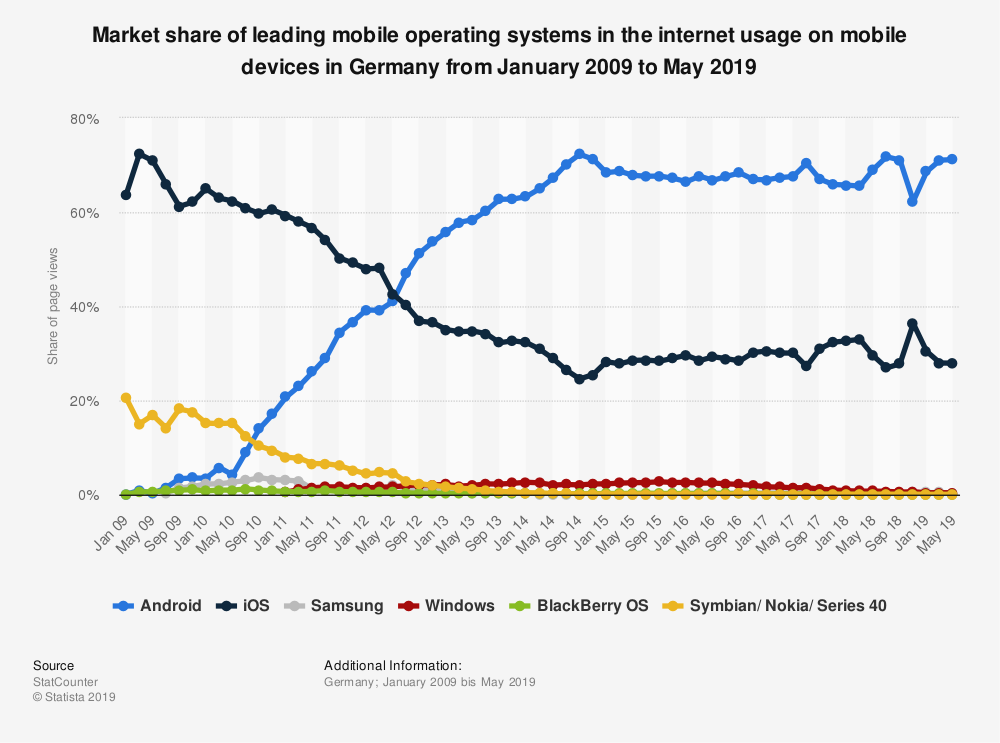
\includegraphics[width=\linewidth]{img/statistic_id461981_market-share-of-operating-systems-in-mobile-internet-usage-in-germany-2009-2019.png}
%        \centering
%        \caption{Market share \cite{StatistaMarketShareSmartphone}}
%        \label{fig:marketshare}
%\end{figure}

%===========================================================================
%	Motivation
%===========================================================================
\section{Motivation dieser Arbeit}
Forschungsfrage: kann \ac{pwa} native App langfristig ablösen

Mobilegeräte Leistungsstärker
Möglichkeiten plattformübergreifend zu entwickeln

Nutzer Conversion kann langfristig gesteigert werden --> Profit!\\
https://developers.google.com/web/progressive-web-apps
\cite{GooglePWAOverview}



%===========================================================================
%	Kapitelübersicht
%===========================================================================
\section{Kapitelübersicht}
In diesem Kapitel (\ref{chap:einleitung}) wurden die aktuellen Marktenwicklungen kurz mit Zahlen benannt und die Motivation dieser Arbeit dargelegt. Das folgende Kapitel 
(\ref{chap:grundlagen} \nameref{chap:grundlagen}) legt vorwiegend technischen Grundlagen für die spätere Implementierung einer Anwendung als PWA und nativer App. Dabei wird auf die verwendeten Technologien und Frameworks eingegangen und speziell die PWA auf technischer Ebene erklärt. 

Kapitel \ref{chap:architektur} (\nameref{chap:architektur}) erläutert die Architektur der entwickelten Anwendung: eine Todoliste. In diesem Kapitel werden detaillierte Spezifikationen beschrieben, die den Entwicklungsprozess erst vergleichbar machen. Außerdem wird auf architekturbezogene Entscheidungen der Plattformen eingegangen, beispielsweise die Gründe für die Wahl der Frameworks der PWA.

Um den Entwicklungsprozess vergleichen zu können, wird in Kapitel \ref{chap:framework} (\nameref{chap:framework}) der Vergleichsprozess beschrieben und Kriterien mit ihrer Gewichtung aufgestellt und erläutert. Anschließend werden im zweigeteilten Kapitel \ref{chap:implementierung} (\nameref{chap:implementierung}) die Implementierungsprozesse der PWA und der nativen App detailliert dokumentiert.

Nach dem Sammeln von Erfahrungen bei den Implementierungen werden in Kapitel \ref{chap:evaluation} (\nameref{chap:evaluation}) beide Technologien mithilfe der in Kapitel \ref{fig:marketshare} erstellten Kriterien verglichen und evaluiert.

Abschließend gibt Kapitel \ref{chap:reflexion} (\nameref{chap:reflexion}) ein Urteil über den Erfolg dieser Arbeit und gibt einen Ausblick auf die Zukunft der PWA.

	
	\addtocontents{toc}{\protect\setcounter{tocdepth}{1}}
	\chapter{Grundlagen}
		\label{chap:grundlagen}
		\section{Begrifflichkeiten}
In der Praxis sind viele, in dieser Arbeit häufig verwendete, Begriffe unterschiedlich belegt. Aus diesem Grund soll im Folgenden eindeutig klargestellt werden, was mit den verwendeten Begriffen tatsächlich gemeint ist.

\begin{description}
	\item [App (plural: Apps)]
		In dieser Arbeit werden Programme die speziell für Smartphones entwickelt wurden als Apps bezeichnet. Implizit wird hiermit auch die Plattform auf Android oder iOS eingrenzt. Der Begriff App zeichnet sich in dieser Arbeit dadurch aus, dass die damit gemeinte Anwendung für den Nutzer sehr einfach zu installieren ist. In der Regel beziehen Nutzer Apps aus einem Shop des Hersteller beispielsweise Apples AppStore und starten diese über ein Icon auf dem Startbildschirm des Betriebssystems.
		
	\item [Webseite, Webanwendung und Web App]
		Der Begriff Webseite wird in dieser Arbeit für HTML-basierte Inhalte verwendet, die der*die Nutzer*in über den Browser abruft.
		
		Die Webanwendung unterscheidet sich dahingehen, dass sie dynamisch auf den Nutzer reagiert und seine Eingaben auswertet und gegebenenfalls den angezeigten Inhalt ändert oder nachlädt. Speziell werden JavaScript basierte Anwendungen in dieser Arbeit als Webanwendung oder Web App bezeichnet. Web App und Webanwendung werden synonym verwendet.
		
		Eine Webseite kann, aber muss keine Webanwendung oder Web App sein.
	
	\item [Progressive Web App]
		Eine Progressive Web App ist eine Webseite und speziell eine Webanwendung oder Web App, welche dynamisch auf den Nutzer reagiert.
		In dieser Arbeit werden Webanwendungen, welche lokal auf einem Gerät installiert werden können als \acf{pwa} bezeichnet. Die PWA kann als Webanwendung oder Web App bezeichnet werden, welche die Kriterien aus Kapitel \ref{chap:pwa} erfüllt.
		
		Im Unterschied zur nativen App kann die selbe PWA sowohl auf Smartphones, als auch auf eine Desktopgerät (Notebook, Desktop Computer etc.) installiert werden.
		
	\item [Desktop PWA]
		Mit Desktop PWA ist hier explizit eine Progressive Web App gemeint, welche auf einem Desktopgerät installiert wird.
			
	\item [native App]
		Diese Arbeit beschäftigt sich mit einer modernen Methode Mobilanwendungen zu programmieren: der \ac{pwa}. Im Unterschied dazu ist eine native App in Java oder Swift geschrieben und ist damit stark plattformabhängig. Nativ implementiere Apps sind entweder für iOS oder Android entwickelt worden, nicht aber für mehrere Plattformen.
		
	\item [Container]
		Da die Entwicklung von Apps stark am Frontend orientiert ist wird häufig der Begriff Container verwendet. Damit ist explizit \textit{kein Container im Sinne von Virtualisierung}, wie beispielsweise ein Docker-Container, gemeint. Der Begriff wird im HTML-Kontext verwendet und meint in dieser Arbeit ein Element, dass andere Elemente beinhaltet.
	
\end{description}

\section{Die Progressive Web App}
\label{chap:pwa}

%\subsection{Charakteristiken einer \ac{pwa}}
Zu Beginn dieses Unterkapitels soll die bereits erwähnte \acf{pwa} erklärt werden. Anschließend folgen die verwendeten Frameworks für die Entwicklung der \ac{pwa}. Ein Überblick über diese ist essenziell für das Verständnis von Kapitel \ref{chap:implementierung}, in welchem die Implementierungsschritte betrachtet werden.

Eine Progressive Web App ist ein nächster Schritt nach der Dynamisierung statischer HTML-Seiten durch JavaScript und Frontendframeworks. Der Software Entwickler und Author Majid Hajian charakterisiert \ac{pwa}s mit acht Eigenschaften. Die wichtigsten dieser Charakteristika werden im Folgenden zusammenfassend erläutert:


\begin{description}
  \item [Installierbarkeit]
	  Der*die Nutzer*in einer Webanwendung kann diese lokal auf seinem Gerät installieren. Sie kann anschließend, wie eine native App, vom Startbildschirm gestartet werden. Um die Webanwendung zu Nutzen muss ein*e Nutzer*in keinen Zwischenschritt mehr über den Browser tätigen.
  
  \item [Ähnlichkeit mit einer nativ implementierten App]  
 	 Klassischerweise werden Android-Apps in Java und iOS Apps in Swift programmiert. Die \ac{pwa} soll, wie eine native App, auf die Hardware des Mobilgeräts zugreifen können (beispielsweise die Nutzung Bluetooth-Chips). Außerdem unterscheidet sich das User Interface der \ac{pwa} nicht maßgeblich von der nativen App. 
  
  \item [Offline-Verwendung] 
  	Die \ac{pwa} soll unabhängig von Netzwerkverbindung funktionieren. Sie ist nach dem "offline-first-design" konzipiert. Die Google-Chrome Dokumentation für Cloud-Entwickler beschreibt Offline First Apps als Webanwendung, deren Dateien (JavaScript, HTML, CSS etc.) bereits heruntergeladen sind. Daten werden temporär über eine Browser-Schnittstelle gespeichert und bei Bedarf synchronisiert. Außerdem kann die Anwendung auf eine unterbrochene Netzwerkverbindungen reagieren \cite{GoogleOfflineApps}. Die \ac{pwa} ist demnach eine Webanwendung, die sowohl online, als auch offline nutzbar ist.

  \item [Mobiloptimiert]  
  	Die \ac{pwa} ist für die (meist leistungsschwache) Mobilhardware konzipiert und funktioniert hierauf ohne Performanceprobleme. Hajian legt besonders auf das schnelle Laden beim Start der Anwendung wert.
  	
  \item [Informierung des*der Nutzers*in] 
  	Wie native Apps, kann die \ac{pwa} den Nutzer über Push-Nachrichten informieren oder zu Interaktion auffordern.
\end{description}

\cite[S. 1f.]{Hajian2019}
Diese Charakteristiken decken sich mit der Beschreibung durch die Entwickler-Dokumentation der \ac{pwa} von Google. Im Vergleich zu Hijian ist diese etwas spezifischer und erwähnt beispielsweise die Kontrolle des Anwendungscaches durch einen JavaScript Service Worker (siehe Kapitel \ref{chap:service_worker}), um die Abhängikeit von einer Netzwerkverbindung aufzuheben.
\cite{GooglePWAOverview}

\subsection{Installation einer Progressive Web App}

Diese Arbeit betrachtet die \ac{pwa}, da sie (wie eine native Anwendung) lokal auf einem Gerät installiert werden kann. Es ist dafür kein zentraler Shop nötig: die Installation wird über den Browser gestartet.

\begin{figure}[h]
        \centering
        
\includegraphics[scale=0.2]{img/a2hs-infobar-cropped.png}
        \caption{Browserdialog zur Installation einer \ac{pwa} \cite{PWAAddToHomeScreenPrompt}}
        \label{fig:pwainstallationprompt}
\end{figure}

Die Aufforderung zur Installation einer \ac{pwa} kann entweder über den Browser (siehe Abbildung \ref{fig:pwainstallationprompt}) erfolgen oder über ein Element der Website, dass ein Event erzeugt, wie beispielsweise ein Button oder ein Dialog. 

Zwar bezeichnen Browser die Installation meist nur als \texttt{Zum Startbildschirm hinzufügen} tatsächlich generiert der Browser aber dann eine WebAPK, welche auf dem Gerät installiert wird. Auf Desktopgeräte startet die \ac{pwa} in einem eignen stark verschlankten Browserfenster ohne Suchleiste und Bedienelemente. \cite{GooglePWAInstallation}


\subsection{Manifest Datei für die Konfiguration der \ac{pwa}}

Um die \ac{pwa} auf einem Gerät installieren zu können, muss es eine web-app-manifest Datei zur Verfügung gestellt werden. Diese ist ein \ac{json} file, welche als Konfigurationsdatei der installierten Anwendung dient. \cite{GooglePWAManifest}

\begin{listing}[H]
    \inputminted{json}{sourcecode/manifest_sample.json}
    \caption{Manifestdatei einer \ac{pwa}}
      \label{sourcecode:manifest_sample}
\end{listing}

Quellcode-Abschnitt \ref{sourcecode:manifest_sample} zeigt den Inhalt einer Manifest-Datei. Neben diversen Icons (Zeile 4-15) werden auch \textit{Name} (Zeile 3), \textit{Farbschema} (Zeile 20) und \textit{Anzeigeeinstellungen} (Zeile 18) festgelegt.
Die Manifest-Datei wird im HTML der Webanwendung eingebunden, siehe Quellcode-Abschnitt \ref{sourcecode:manifest_include}. 

Es ist die Einfachheit dieses Prozesses hervorzuheben: Das Hinzufügen einer (wenige Zeilen langer) \ac{json}-Datei macht die gesamte Webanwendung installierbar. Es wird kein App-Store, manueller Dateidownload oder Installer benötigt. 

\begin{listing}[H]
    \inputminted{xml}{sourcecode/include_manifest.html}
    \caption{Einbinden der Manifestdatei}
      \label{sourcecode:manifest_include}
              %https://developers.google.com/web/fundamentals/web-app-manifest?hl=en
\end{listing}

%\begin{figure}[h]
%        \centering
%%        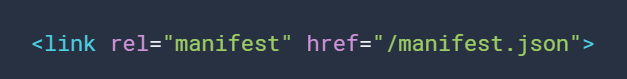
\includegraphics[scale=0.7]{img/include_manifest.png}
 %%       \caption{Einfache Einbindung des Manifests}
  %      \label{sourcecode:manifest_include}
        %https://developers.google.com/web/fundamentals/web-app-manifest?hl=en
%\end{figure}


\subsection{Service Worker für Offline-Funktionalität und Benachrichtigungen}
\label{chap:service_worker}

Damit die \ac{pwa} trotz fehlender Netzwerkverbindung funktioniert wird ein besonderer Mechanismus benötigt: der Service Worker. Mit ihm können Abhängigkeiten der App lokal gecached werden, so dass die Anwendung auch bei schlechter oder gar fehlender Netzwerkverbindung funktioniert. \cite[S. 7]{BeginningPWA}

Ein Service Worker ist ein von der UI seperiertat laufendes Hintergrundskript der Webanwendung, siehe Abbildung \ref{fig:serviceWorker}. Er wird genutzt um Bilder, Skripte, Styles oder ganze Seiten zu cachen. Bei bestehender Netzwerkverbindung führt er nötige Synchronisierungen durch. Nicht zuletzt ist er auch für das senden von Push-Notifications zuständig. \cite[S. 24]{BeginningPWA}

\begin{figure}[h]
        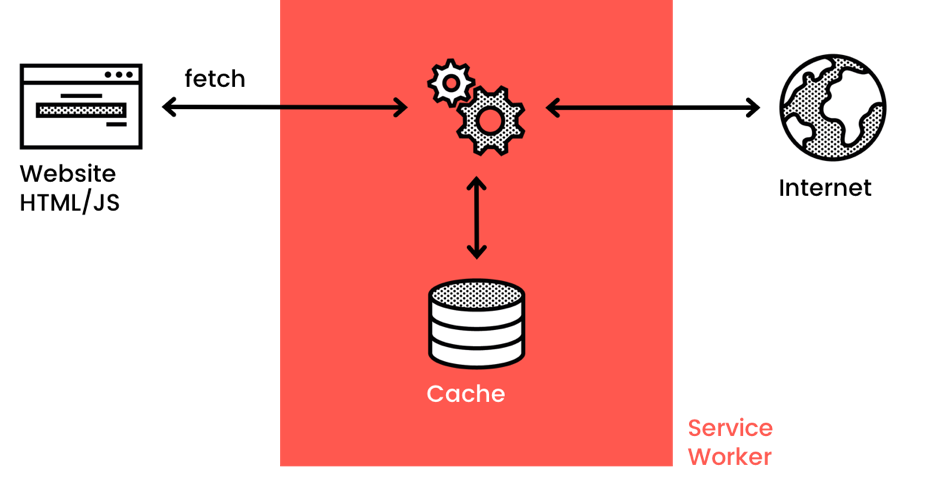
\includegraphics[width=\linewidth]{img/ServiceWorker-8a0968f1b295f1ff.png}
        \centering
        \caption{Konzept des Service Workers \cite{ServiceWorkerDiagramm}}
        \label{fig:serviceWorker}
\end{figure}


Alle verbreiteten Desktopbrowser wie Chrome, Firefox, Opera, Edge und mitterweile auch Safari unsterstützen das Service Worker Konzept. Der Mobile Chromebrowser unter Android unterstützt Service Worker bereits voll, während Safari unter iOS noch an diesem Feature arbeitet. \cite[S. 9]{BeginningPWA}


\subsection{Plattformen von eine \ac{pwa} aktuell unterstützen}
Das Projekt \textit{CanIUse} aggregiert Daten zu Webstandards des w3 Konsortiums und Browserdokumentationen. Es wird als Quelle für die Unterstützung von Features durch aktuelle Browser herangezogen.

Apples mobiler Browser Safari unterstützt eines der wichtigsten Features der \ac{pwa} noch nicht vollständig: das Web App Manifest. Allerdings wird der Service Worker vollständig unterstützt \cite{CanIUseWebManifest}. Wann und ob Safari die Unterstützung für das Manifest implementiert ist unklar und bleibt abzuwarten. Die aktuelle Teilunterstützung zeigt jedoch, dass sich Apple nicht grundsätzlich gegen die \ac{pwa} weigert.

 %Die Versionen zeigen aber eine stetig voranschreitende Integration der, erweitert den Funktionsumfang in den neusten Versionen von iOS. 

% https://medium.com/@firt/progressive-web-apps-on-ios-are-here-d00430dee3a7



% Source: https://developers.google.com/web/progressive-web-apps/desktop
Die Nutzung von \ac{pwa}s ist nicht ausschließlich auf Smartphones begrenzt. Wie normale Desktopprogramme werden Desktop \ac{pwa}s in einem eigenen Fenster gestartet. 
Der Unterschied zwischen den Bedienelementen nativer Desktopanwendungen und Desktop \ac{pwa}s ist ausschließlich farblicher Natur. Stark vereinfacht beschrieben, sind Desktop \ac{pwa}s Browserfenster ohne Tabs und Adressleiste. Durch die Nutzung von Service Workern, welche die Webanwendung cachen, sind auch Desktop \ac{pwa}s nicht an eine Netzwerkverbindung gebunden.

Grundsätzlich können Desktop \ac{pwa}s auf jedem Betriebssystem installiert werden, auf dem Google Chrome (Version größer 73) installiert werden kann: Windows, Mac, Linux und Chrome OS.
\cite{GooglePWADesktop}



\subsection{Grundlage der Webanwendung: JavaScript Laufzeitumgebung Node.js}

%NodeJSWebsiteAbout
Node.js ist eine open-source JavaScript Laufzeitumgebung für die Entwicklung skalierbarer Webanwendungen 
\cite{NodeJSWebsiteAbout}.
Selbst baut Node.js auf der V8-Engine auf, einer Laufzeitumgebung, die auch von Google Chrome genutzt wird 
%NodeJSRecepies
\cite[S. 1]{NodeJSRecepies}.
% PracitalNodeJS
Wegen zeitsparenden Features, wie automatischem Typecasting oder der Tatsache, dass Node.js alle Daten als Objekt behandelt, erfreut sich Node.js großer Beliebtheit 
\cite[S. 12]{PracitalNodeJS}.
Die Kombination mit dem Package Manager npm ermöglicht die einfache Installation und Nutzung von Modulen, um die Funktionalität der Plattform zu erweitern. 
\cite[S. 9]{NodeJSRecepies}.


\subsection{Frontend-Framwork Angular für die Entwicklung von Webanwendungen}

Angular ist ein open-source TypeScript basiertes Framework zur Entwicklung von Webanwendungen, welches Node.js nutzt.


%https://octoverse.github.com/projects
Mit über Achttausend Mitwirkenden Entwicklern (Angular CLI) beziehungsweise über Siebentausend Mitwirkender (Angular Framework) belegt das Angular Command Line Interface und das Angular Framework die Plätze 4 und 6 der größten Projekte auf Github. 
% https://octoverse.github.com/projects
\cite{OctoverseGitHubStatistics}

Das Framework arbeitet auf Basis von Komponenten. Ein Eingabefeld, Seite oder eine Liste werden in Angular als solche Komponenten seperat betrachtet. Auch in der Dateistruktur werden Komponenten stark getrennt. Jede Komponente besitzt beispielsweise ein eigenes CSS (oder SCSS) und HTML-File. Eine Komponente für eine Seite kann so auch eine oder sogar mehrere Listenkomponenten einbinden. Durch die Wiederverwendung von Code-Fragmenten in Komponenten wird der Programmcode sehr übersichtlich und strukturiert.

\begin{figure}[h]
        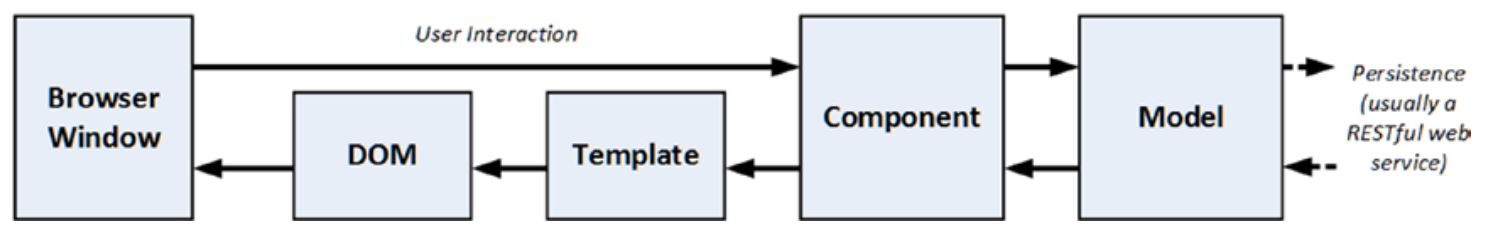
\includegraphics[width=\linewidth]{img/Angular_MVC.JPG}
        \centering
        \caption{MVC Konzept von Angular \cite[S. 35, Abbildung 3-4]{ProAngular}}
        \label{fig:angularmvc}
\end{figure}

Eine Angular Anwendung ist in drei Einheiten gegliedert:\\

\textbf{Model}\\ 
Enthält Logik für die Verwaltung von Daten, beispielsweise das Erstellen, Speichern oder Modifizieren. Dies kann über die Kommunikation mit einem Webserve via REST-API erfolgen. Das Model enhält keine Logik, um mit dem Nutzer zu interagieren.\\

\textbf{Component}\\
Enthält Logik für das Aktualisieren der Daten im Model aufgrund Nutzerinteraktion. \\

\textbf{Template}\\ 
Enthält Logik und Markup, um dem Nutzer Daten anzeigen zu können.

\cite{ProAngular}

\section{native Apps}


\subsection{Apple iOS} \label{chap:apple_ios}

iOS ist ein Betriebssystem, welches vom US-amerikanischen Technologiekonzern \textit{Apple, Inc.} im Rahmen des erstmalig vorgestellten \textit{iPhones} im Jahre 2007, damals noch unter dem Namen \textit{iPhone OS}, in Umlauf gebracht wurde. Stand heute läuft dieses Betriebssystem ausschließlich auf den Mobilgeräten des genannten Herstellers. Neben dem iPhone nutzt auch das Multimedia-Gerät \textit{iPod touch} das Betriebssystem iOS. Der Tabletcomputer \textit{iPad} wurde bis September 2019 ebenfalls über iOS betrieben, besitzt jedoch seit der Umstellung ein eigenes, an iOS stark angelehntes Betriebssystem \textit{iPadOS}.

\subsubsection{Entwicklung von iOS-Applikationen}

In seiner ersten Version stellte iPhone OS noch keinerlei Möglichkeit bereit, Anwendungen von Drittanbietern bereitzustellen sowie zu nutzen. Dies änderte sich bei der Umbenennung des Betriebssystems in iOS im Jahre 2008, welche auch ein Software-Update zur Folge hatte, in welchem diese Eigenschaft nun geboten wurde.

\paragraph{Programmiersprache: Apple \textit{Swift}}\mbox{}\\
In der Anfangszeit der Anwendungsentwicklung für iOS wurde die bereits für andere Zwecke entwickelte und vorhandene Programmiersprache \textit{Objective-C} als Standard gewählt. Dies änderte sich im Jahre 2014, als Apple bei seiner jährlichen Entwicklerkonferenz die hauseigene Programmiersprache \textit{Swift} vorstellte, welche Objective-C in der ganzheitlichen Anwendungsenwicklung rund um Apple-Geräte ablösen sollte. In der Anfangszeit von Swift war diese immer noch stark an den Vorgänger Objective-C angelehnt. Über die Zeit sank der Einfluss, jedoch ist Swift weiterhin abwärtskompatibel zu Objective-C, welche wiederum abwärtskompatibel zu C ist.

Bei Swift handelt es sich um eine objekt- und protokoll-orientierte Programmiersprache, welche in Ihren verschiedenen Anwendungsbereichen ihre Zugehörigkeit zu verschiedenen Programmierparadigmen aufweist. Diese stützt sich vor allem auf ihrer Behauptung, möglichst leicht verständlich für einen Menschen zu sein und vermeidet bekannte Probleme anderer, populärer objektorientierter Programmiersprachen, bspw. Dereferenzierung von \texttt{null}\textit{-Pointer-Exceptions}.

Neben der Entwicklung für alle Apple-Plattformen wird Swift unter anderem auch zur Back-End-Entwicklung genutzt. Laut einer Umfrage von \textit{StackOverflow} positioniert sich Swift auf Platz 14 der beliebtesten Programmiersprachen, basierend auf 8,1\% aller Stimmen.

\paragraph{Entwicklungsumgebung: Apple \textit{Xcode}}\mbox{}\\
\textit{Xcode} ist eine, ebenfalls von Apple entwickelte, sog. integrierte Entwicklungsumgebung (engl. \ac{ide}) und wird primär für die Entwicklung von Anwendungen mit der Programmiersprache Swift eingesetzt. Grundsätzlich ist Xcode, und somit auch die Programmierung mit Swift, Apple \textit{Mac}-Nutzern vorbehalten. Über die Zeit wurden weitere \acp{ide} entwickelt, welche Swift unterstützen, denen jedoch grundlegende, nachfolgend beschriebene Funktionalitäten von Xcode, fehlen. Zu nennen ist hier bspw. die Lösung \textit{AppCode} des Unternehmens \textit{JetBrains}.

Xcode unterstützt neben Swift auch die abwärtskompatiblen Programmiersprachen Objective-C, C, aber auch C++, Python, Ruby, sowie andere. Darüber hinaus bietet Xcode einen sog. \textit{Interface Builder}, mit welchem das Frontend über separate Ansichten (sog. \textit{Views}) vorbereitet werden kann. Dabei werden verschiedenste Komponenten bereitgestellt, welche via \textit{Drag'n'Drop} innerhalb der Ansichten platziert und optisch konfiguriert werden können. Auch Beziehungen zwischen den einzelnen Views können bereits hier angelegt werden. Ein Beispiel für die Nutzung des Interface Builders kann dem unten stehenden Screenshot entnommen werden.

\begin{figure}[h!]
	\centering
	\caption{Nutzung des Interface Builders in Xcode}
\end{figure}

% Erklärung des Screenshots
Die zusammengesetzten Komponenten können, ebenfalls über Drag-and-Drop in den Quellcode referenziert werden, um die Verhaltensweisen dieser programmatisch festzulegen. Ist die App in einem testreifen Zustand, kann diese direkt über Xcode emuliert werden. Es öffnet sich ein sog. \textit{Simulator}, welcher das Zielgerät mit der geöffneten Anwendung darstellt. Das Verhalten und etwaige, daraus resultierende Probleme, können somit erkannt werden, ohne, dass es ein tatsächliches, physikalisches Zielgerät bedarf. Eigenschaften, welche auf die Hardware-Komponenten des Geräts zugreifen (bspw. die eingebauten Kameras, den Bluetooth-Sensor, etc.) können mit Ausnahme der Netzwerkkarte nicht simuliert werden.

\paragraph{Softwaredesign-Muster \textit{Model-View-Controller}}\mbox{}\\ 
Apple empfiehlt als grundlegendes Prinzip für die App-Entwicklung mit Swift das Muster \textit{\ac{mvc}}, welches im Folgenden aufgeschlüsselt wird.

\begin{description}
	\item[Model] (dt. \textit{Modell} bezieht sich auf das Datenmodell und die datenbedingte Kommunikation innerhalb der Anwendung. Innerhalb von der iOS-Anwendungsentwicklung finden sich hier Quellcode-Abschnitte für die Kommunikation der App mit einer potenziellen \acs{api}, Code für die Definition und Bereitstellung von persistentem Speicher sowie die Handhabung der dadurch entstehenden Daten. Auch im Quellcode verwendete Konstanten sind dem Modell zuzuschreiben.
	\item[View] (dt. \textit{Präsentation}) bezieht sich auf die Frontend-Komponenten der Anwendung. Alle durch den Interface Builder spezifizierten Eigenschaften sind der Präsentation zuzuschreiben, also jegliche Komponenten, frontend-basierte Klassen sowie Animationen.
	\item[Controller] (dt. \textit{Steuerung}) beinhaltet die spezifische Verhaltenslogik der Anwendung bei Interaktion mit dieser durch den Nutzer. Vereinfacht formuliert bestimmt dieser, welche Funktionalität zu welcher Zeit auf Basis welches Verhaltens ausgeführt wird. Diese ist ebenfalls für die Kommunikation zwischen dem Modell und der Präsentation zuständig.
\end{description}

Die Kooperation der einzelnen Komponenten dieses Musters lässt sich anhand der unten stehenden Abbildung erläutern.

\begin{figure}[h!]
	\centering
	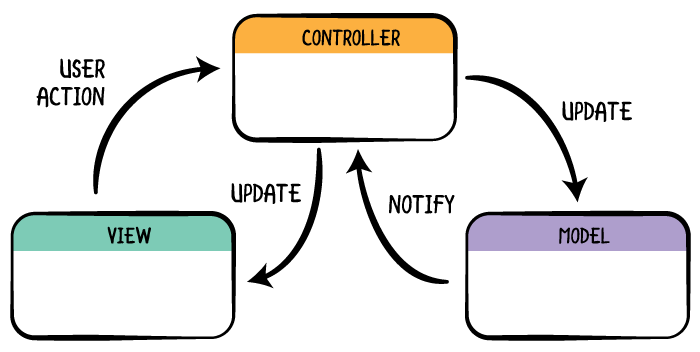
\includegraphics[width=0.5\linewidth]{img/mvc}
	\caption{Zusammenspiel des \ac{mvc}-Musters}
\end{figure}

% Erklärung MVC-Grafik

Technisch wird dieses Muster durch die Verknüpfung der einzelnen (durch den Interface Builder bereitgestellten oder erstellten) Views mit spezifischen, sog. \textit{View Controllern} realisiert. Durch eine Aktion des Nutzers auf dem View wird die entsprechende Funktionalität über den View Controller bereitgestellt. Dieser kann dann ebenfalls Funktionen ausführen, welche durch das Modell bereitgestellt werden, falls die Aktion dies bedarf. Die entsprechenden Klassen der View Controller sind Unterklassen der einzelnen, spezifischen Views, welche deren vorgesetzte Basisfunktionalitäten um die gewünschten Funktionen des Entwicklers erweitern.

\paragraph{Vorbereitung der Projektumgebung}\mbox{}\\
Bei der Erstellung eines neuen Projektes innerhalb von Xcode wählt der Entwickler bereits zu Beginn bestimmte Spezifikationen für die zu entwickelnde Anwendung. Da Swift auch für andere Betriebssysteme von Apple zur Anwendungsentwicklung genutzt wird, gehört die Spezifizierung des Anwendungsbereiches (hier: iOS) sowie des grundlegenden Aufbaus der App zu den Vorbereitungsmaßnahmen der Projektumgebung. Dieses Dialogfenster kann aus dem unten stehenden Screenshot entnommen werden.

\begin{figure}
	\centering
	\caption{Dialogfenster zum Anlegen eines neuen Projektes (Xcode)}
\end{figure}

Letztere bereiten verschiedene Dateitypen innerhalb der Umgebung vor, bspw. verschiedene Ansichten mit bereits integrierter Navigation, welche bei einer Anwendung mit nur einer Ansicht nicht zu tragen kommen. Im zweiten Schritt der Projektvorbereitung trifft der Entwickler Entscheidungen über Projektverzeichnis, -namen und -sprache sowie über weitere Projektkomponenten, welche für die Anwendung von Bedarf wären.

Alle hier getroffen Schritte können auch manuell bzw. im Nachgang der Projekterstellung angelegt werden. Grundsätzlich sind die Dateien und Quellcodezeilen, welche durch die genannten Vorbereitungsmaßnahmen automatisch generiert werden, unabdingbar für die Realisierung des Projekt und können somit für eine effizientere Arbeit des Entwicklers sorgen.

\paragraph{Struktur des initialen Entwicklungsverzeichnisses}
Bereits zu Anfang befinden sich bestimmte Dateien im Entwicklungsverzeichnis, welche sich grundsätzlich in jeder iOS-Anwendung benötigt werden. Diese werden im Folgenden beschrieben.

\begin{description}
	\item[\texttt{AppDelegate.swift}] ist der Eintrittspunkt der App. Dieser ist zuständig für das Verhalten der App, wenn diese (zum ersten Mal) geöffnet, geschlossen oder in den Hintergrund gerückt (d.\ h. inaktiv gesetzt) wird. Diese Datei ist vor allem dann von Interesse, wenn die Anwendung auch außerhalb ihrer Aktivität bestimmte Funktionen ausführt, bspw. also bei Musik-Anwendungen oder Stoppuhren. Aufgrund der automatischen Bereitstellung von Core Data zu Anfang des Projektes ist hier auch das Grundgerüst des \textit{Persistent Service} zu finden.
	\item[\texttt{SceneDelegate.swift}] ähnelt dem \texttt{AppDelegate} sehr, bezieht sich jedoch auf das Verhalten der Ansicht(-en) der Anwendung. Diese wird benötigt, da seit iOS-Version 13 auch mehrere offene Instanzen derselben App möglich sind, welche jedoch immer den aktuellsten Zustand darstellen sollen, unabhängig von der gerade aktiv laufenden Instanz. In Form einer Analogie aus der Web-Entwicklung kann man den \texttt{SceneDelegate} als die oberste Hierarchie der \textit{Frontend}-Steuerung bezeichnen, während das \textit{Back End} über den \texttt{AppDelegate} orchestriert wird.
	\item[\texttt{ViewController.swift}] ist einer von beliebig vielen möglichen Controllern, welche direkte Anbindung zu einer oder mehreren Ansichten hat. Dieser beinhaltet Konfigurationen der verschiedenen Komponenten der Ansicht und spezifiziert auch das Verhalten der Ansicht, wenn auf diese oder von dieser gewechselt wird.
	\item[\texttt{Main.storyboard}] ist das Gegenstück zu den \texttt{ViewController}. In Form eines sog. \textit{Interface Builders} können verschiedene Ansichten und deren Verknüpfungen via \textit{Drag-and-Drop} erstellt werden. Jede Ansicht wird mit genau einem \texttt{ViewController} versehen, welcher die Steuerung der definierten Elemente übernimmt. Grundsätzlich ist es auch möglich, vollständig ohne Interface Builder auszukommen. Die initiale Konfiguration der Positionen und der weiteren optischen Eigenschaften wird dann ebenfalls über den entsprechenden \texttt{ViewController} gehandhabt, wobei dies einen deutlich höheren Programmieraufwand aufweisen könnte. Neben des \texttt{Main.storyboard} existiert auch ein \texttt{LaunchScreen.storyboard}, welcher beim Laden der Anwendung ausgeführt wird.
	\item[\texttt{Assets.xcassets}] beinhaltet das App-Logo, welches im Menü des Mobilgerätes angezeigt wird. Dieses muss in fest definierten Größen bereitgestellt werden, wird jedoch an dieser Stelle vernachlässigt. Darüber hinaus können hier auch alle weiteren Grafiken, etc., abgelegt werden, welche innerhalb der App genutzt werden, um für eine ordnungsgemäße Skalierung der Symbole je nach Bildschirmgröße des Endgeräts zu gewährleisten.
	\item[\texttt{Info.plist}] ist eine allgemeine Konfigurationsdatei. Diese wird u.a. für Berechtigungen genutzt, welche die Anwendung außerhalb ihres eigenen Handlungsspielraums haben soll, bspw. die Nutzung der eingebauten Kameras, des GPS-Standortes des Geräts, die Berechtigung, Benachrichtigungen anzuzeigen, etc.
	\item[\texttt{to\_do.xcdatamodeld}] stellt die Konfigurationsdatei des Persistent Service dar, sofern dieser im Dialogfenster aktiviert wurde. In dieser werden Entitäten angelegt, mit möglichen Relationen versehen und für die Verwendung innerhalb der App exportiert.
\end{description}

\subsubsection{Vertrieb von iOS-Applikationen}
Der mit iOS 2.0 (Nachfolger von iPhone OS) ins Leben gerufene Apple \textit{App Store} ist die einzige offizielle Bezugsstelle für iOS-Applikationen. Somit ist es auch der am meisten verwendete Marktplatz, in welchem Entwickler und Unternehmen ihre Anwendung kostenlos sowie kostenpflichtig zum Download anbieten.

Zunächst ist die Anmeldung des Entwicklers als \textit{Apple Developer} im Vorhinein erforderlich. Ohne diese könnte die Anwendung zwar programmiert und innerhalb der Entwicklungsumgebung getestet, jedoch nicht auf tatsächlichen iOS-Geräten getestet und zum Download freigegeben werden. Dies hat sowohl sicherheitstechnische als auch wirtschaftliche Gründe, welche hier nicht weiter diskutiert, jedoch für die Evaluation der Entwicklungsfreiheit in Betracht gezogen werden. Letzteres erkennt man vor allem an der Tatsache, dass die Verbreitung von Anwendungen über den \textit{App Store} kostenpflichtig ist.

% Evtl. Quelle für die App-Publikation (iOS) finden und zitieren
Der genaue Prozess der Publikation von iOS-Applikationen kann im Rahmen dieser Arbeit nicht nachvollzogen werden, da keine Möglichkeit der tatsächlichen Bereitstellung der zu entwickelnden Beispielanwendung vorliegt.

\subsubsection{Nutzung von iOS-Applikationen}
Wie im vorigen Abschnitt erwähnt werden iOS-Anwendungen über den App Store bezogen. Auf weitere, inoffizielle und teils nonkonforme Praktiken wie das sog. \textit{Jailbraking} des Gerätes, um auch nicht-authorisierte Anwendungen herunterladen und nutzen zu können, wird hier nicht eingegangen.

Der iOS-Nutzer sucht über den App Store die gewünschte App und lädt diese herunter. Für diesen Prozess ist eine sog. \textit{Apple ID}, also ein Benutzerkonto bei Apple vonnöten. Sollte die gewünschte App kostenpflichtig sein, so müssen Kreditkarten- oder anderweitige, valide Zahlungsdaten dem Konto hinterlegt sein. Der Nutzer bestätigt den Kauf bzw. erstmaligen Download über das Benutzerkontenpasswort oder eine gerätespezifische Authentifizierungsmethode (bspw. Fingerabdruck-Erkennung via \textit{Touch ID} oder Gesichtserkennung via \textit{Face ID}, sofern vorhanden). Daraufhin startet der Download. Die App kann über ihr korrespondierendes App-Symbol, welches nun auf dem Menü-Bildschirm des Geräts erscheint, geöffnet werden.

Falls die App in einer nun aktuelleren Version vorliegt, wird diese entweder über den App Store automatisch im Hintergrund neu heruntergeladen. Andernfalls kann der Nutzer diesen Schritt auch manuell über den App Store in Kraft setzen.



\subsection{Android}

\textbf{Entwicklung}

%Android apps are written in Java and use various Java application program interfaces (APIs).
%Because you’ll want to write your own apps, but may be unfamiliar with the Java language and these
%APIs, this book teaches you about Java as a first step into Android app development. It provides you
%with Java language fundamentals and Java APIs that are useful when developing apps.

Native Android Anwendungen werden in Java entwickelt. Durch die Nutzung der zahlreichen APIs wird aus einem Java Programm eine native Android App.
\cite[S. 1]{JavaForAndroid}
Mittlerweile wird die teilweise veraltete Java-Syntax graduell durch die modernere Programmiersprache Kotlin abgelöst.
\cite{KotlinAndroid}


%Kotlin is a free and open source project under the Apache 2.0 license
%https://developer.android.com/kotlin

%https://kotlinlang.org/docs/reference/android-overview.html

Meist werden Android Apps mithilfe der Entwicklungsumgebung Android Studio entwickelt, welches auf der IntelliJ IDE von JetBrains aufbaut, aber von Google weiterentwickelt wird. Die IDE bietet Entwicklern unter anderem einen visuellen Layout-Editor und eine Vielzahl von Android Emulatoren zum Testen der Apps auf verschiedenen Android Versionen und unterschiedlicher Hardware. Dafür wird jedoch performante Hardware zum Entwickeln benötigt: 8 Gigabyte Arbeitsspeicher oder mehr ist die Empfehlung der Herausgeber. \cite{AndroidStudio}

\textbf{Vertrieb}

Die meisten Apps beziehen Nutzer über den Google Play Store, einem Onlineshop für kostenlose und kostenpflichtige Android Anwendungen. 
Updates werden ebenfalls über den Play Store installiert. Alternativ kann ein Nutzer eine App in Form einer \texttt{.apk}-Datei installieren. Dieser Weg bleibt jedoch aufgrund der Umständlichkeit und bedenklicher Sicherheit der App weitestgehend ungenutzt.




\subsection{Android}

\textbf{Entwicklung}

%Android apps are written in Java and use various Java application program interfaces (APIs).
%Because you’ll want to write your own apps, but may be unfamiliar with the Java language and these
%APIs, this book teaches you about Java as a first step into Android app development. It provides you
%with Java language fundamentals and Java APIs that are useful when developing apps.

Native Android Anwendungen werden in der Regel in Java entwickelt. Durch die Nutzung der zahlreichen APIs wird aus einem Java Programm eine native Android App.
\cite[S. 1]{JavaForAndroid}
Mittlerweile wird die teilweise veraltete Java-Syntax graduell durch die modernere Programmiersprache Kotlin abgelöst.
\cite{KotlinAndroid}


%Kotlin is a free and open source project under the Apache 2.0 license
%https://developer.android.com/kotlin

%https://kotlinlang.org/docs/reference/android-overview.html

Meist werden Android Apps mithilfe der Entwicklungsumgebung Android Studio entwickelt, welches auf der IntelliJ IDE von JetBrains aufbaut, aber von Google weiterentwickelt wird. Die IDE bietet Entwicklern unter anderem einen visuellen Layout Editor und eine Vielzahl von Android Emulatoren zum Testen der Apps auf verschiedenen Android Versionen und unterschiedlicher Hardware. Dafür wird jedoch performante Hardware zum Entwickeln benötigt: 8 Gigabyte Arbeitsspeicher oder mehr ist die Empfehlung der Herausgeber. \cite{AndroidStudio}

\textbf{Vertrieb}

Die meisten Apps beziehen Nutzer über den Google Play Store, einem Onlineshop für kostenlose und kostenpflichtige Android Anwendungen. 
Updates werden ebenfalls über den Play Store installiert. Alternativ kann ein Nutzer eine App in Form einer \texttt{.apk}-Datei installieren. Dieser Weg bleibt jedoch aufgrund der Umständlichkeit und unbekannten Sicherheitsprüfung der App weitestgehend ungenutzt.

	\addtocontents{toc}{\protect\setcounter{tocdepth}{2}}
	\chapter{Wissenschaftliches Framework}
		\label{chap:wissenschaftliches_framework}
		%===========================================================================
%	III. Wissenschaftliches Framework
%===========================================================================

Die Grundlage für eine adäquate Bewertung der zu entwickelnden mobilen Anwendungen bildet die Definition beidseitig anwendbarer, quantifizierender Kriterien. Die Notwendigkeit hierin begründet sich darin, dass kein allgemein anerkannter Kriterienkatalog für die Pauschalisierung von Softwarequalität existiert. Viel eher benötigen unterschiedliche Projekte mit unterschiedlichen Schwerpunkten eine unterschiedlich definierte Definition der entsprechenden Gesichtspunkte.

Wie zuvor erwähnt wird die Forschungsfrage, ob \acp{pwa} native Apps langfristig ersetzen können, vor allem auf Basis der Umsetzbarkeit in der Entwicklung evaluiert. Umgekehrt könnten ähnliche Fragestellungen anhand wirtschaftlicher Aspekte begründet werden (bspw. Anzahl der benötigten Entwickler, preislicher Rahmen, Profitmöglichkeiten, etc.). Bei der Einfachheit der Beispielanwendung haben solche Aspekte jedoch kaum Bedeutung. Ebenfalls in Betracht gezogen werden muss die Tatsache, dass die Verfasser dieser Studienarbeit keine erfahrenen Entwickler ersetzen, weswegen auch quantifizierende Kriterien wie die Dauer der Entwicklungszeit, etc., keine Anwendung in der zugrunde liegenden Bewertung finden können. Gleiches gilt ebenfalls für die nur empirisch evaluierbaren Punkte der Nutzung seitens der Anwender (z.B. Intuitivität, Benutzerfreundlichkeit, Anspruch der Gestaltung, etc.), da eine solche Studie den Rahmen dieser Arbeit verlassen würde.

Bezüglich der Umsetzung in der Entwicklung lassen sich jedoch mehrere Kriterien aufstellen, die zur Beantwortung (oder zumindest Lenkung) der Forschungsfrage beitragen können. Die Definition der allgemeinen technischen Architektur in Kapitel \ref{chap:architektur} der zu entwickelnden Mobilanwendung geschieht unter Berücksichtigung der Kriterien, um eine neutrale Vergleichbarkeit zu ermöglichen.

\section{Vorgehen bei der Bewertung}
Um die Entwicklungen der Angular-\ac{pwa} und der nativen iOS-App zu vergleichen, wird die im Folgenden beschriebene Kriteriengewichtung (siehe Tabelle \ref{tab:punktekatalog}) verwendet. Einzelne Kriterien werden anhand Tabelle \ref{tab:verrechnungspunkte} bewertet und die Verrechnungspunkte anschließend über alle betrachteten Kriterien aufsummiert.

\begin{table}[h!]
	\centering
	\begin{tabular}{|c|c|c|c|c|c|}
		\hline 	
			\textbf{Bewertung} & $--$ & $-$ & \Circle & $+$ & $++$ \\ 
		\hline 
			\textbf{Beschreibung} & schlecht & eher schlecht & neutral & eher gut & gut \\ 
		\hline 
			\textbf{Verrechnungspunkte} & $-2$ & $-1$ & $0$ & $1$ & $2$ \\ 
		\hline 		
	\end{tabular} 
	\caption{Verrechnungspunkte} \label{tab:verrechnungspunkte}
\end{table}

Das Ergebnis ist eine Evaluationsmatrix, welche als Netzdiagramm dargestellt die bewerteten Kriterien einzeln visualisiert und eine Gesamtbewertung pro Technologie liefert. In diese fließen die Kriterien einzeln ein und bilden ein Gesamtbild. Die Gewichtung der Kriterien ist in Tabelle \ref{tab:punktekatalog} dargestellt.

\begin{table}[h!]
	\centering
	\begin{tabular}{|l|c|}
		\hline
		Kriterium              & Gesamtanteil \\
		\hline
		\multicolumn{2}{c}{Anwendung}     \\
		\hline
		Plattformabhängigkeit   & 10\%         \\
		Installation           & 5\%          \\
		Speicherzugriff        & 5\%          \\
		Speicherbedarf         & 5\%          \\
		Aktualisierbarkeit     & 5\%          \\
		Konsistenz des Designs & 5\%         \\
		
		\hline
		\multicolumn{2}{c}{Entwicklung}     \\
		\hline
		Bibliotheken           & 10\%         \\
		Umsetzung              & 20\%         \\
		Testbarkeit            & 10\%         \\
		Vorausgesetzte Entwicklungserfahrung    & 10\%         \\
		\hline
		\hline
		Summe                  & 100\%        \\
		\hline
	\end{tabular}
	\caption{Kriteriengewichtung} \label{tab:punktekatalog}
\end{table}

\section{Betrachtete Aspekte der Entwicklung}
Bei der Evaluation soll auf verschiedene Aspekte beider Projekte eingegangen werden. Diese lauten wie folgt:
\begin{description}
	\item [Anwendung]
		Die Kriterien zur Anwendung (bzw. App) beziehen sich auf die Eigenheiten der Apps, darunter die Installation, die Aktualisierung und die Plattformabhängigkeit.
		
	\item [Entwicklung]
		Kriterien der Entwicklung beziehen sich auf die Programmierung und Umsetzung der funktionalen und nicht-funktionalen Anforderungen.
			
\end{description}


Grundsätzlich gibt es einen Punktabzug, wenn der Nutzer grundlegenden Funktionen explizit zustimmen muss. Das Idealbild ist eine sofort nutzbare Anwendung, die ohne weitere Zwischenschritte den kompletten Funktionsumfang besitzt.

\section{Betrachtete Kriterien}
Die einzelnen Kriterien aus der Evaluationsmatrix werden nun genauer definiert:

\begin{description}
	\item [Plattformabhängigkeit] 
		  Unterstützt die Anwendung mehrere Plattformen, also beispielsweise Android und iOS wird dies als gut bewertet. Ist die Anwendung auch auf Desktop-Computern oder Tablets nutzbar, gibt dies ebenfalls eine positive Bewertung.
		  
	\item [Installation]
	      Die App sollte ohne mehrere Zwischenschritte nutzbar sein. Ist die Installation zu kompliziert, führt dies zu Punktabzug.

	      Es fließt mit ein, wie viel Aufwand betrieben werden muss, um die App einem Publikum zur Verfügung zu stellen. Dieser Aufwand ist idealerweise gering und im Interesse des Entwicklers.

	\item [Speicherzugriff]
	      Anwendungen müssen Daten speichern können, um dem Nutzer einen Mehrwert zu bieten. Die Größe der zu speichernden Daten ist bei diesem Vergleich auf einige Kilobyte begrenzt. Gibt es die Möglichkeit Dateien abzulegen, ist dies positiv zu werten. Idealerweise können Daten in gängigen Formaten (beispielsweise \acsu{json}, \acsu{csv}, \acsu{xml} oder Plaintext) gespeichert werden.
	      Können Daten nur temporär und nicht persistent gespeichert werden, führt dies zu starkem Punktabzug. Muss der Nutzer dem Speichern von Daten aktiv zustimmen, stört dies die Nutzungserfahrung und ist daher negativ zu werten.

	\item [Speicherbedarf]
	      Der Speicherplatz eines Smartphones ist deutlich kleiner, als der eines Desktop-Computers. Bestenfalls ist die Anwendung nur einige Megabyte groß und kann so schnell über eine mobile Datenverbindung installiert und upgedatet werden \cite{AppleMaxAppSize} \cite{GoogleMaxAppSize}. 
	      Hoher Speicherverbrauch führt zu Punktabzug, wohingegen geringer Speicherverbrauch positiv bewertet wird. Der Verbrauch ist unter den einzelnen Plattformen relativ zu bewerten.

	\item [Aktualisierbarkeit]
	      Idealerweise kann die Installation von Updates vom Entwickler kontrolliert werden. Schnelle Updatezyklen sind wünschenswert, da in der Praxis dadurch schnell Sicherheitslücken und Bugs behoben werden können. Wenn ein Nutzer sich aktiv gegen Updates weigern kann, oder diese manuell installieren muss, könnte dies für Kompatibilitätsprobleme mit Webschnittstellen oder Sicherheitsprobleme sorgen und führt deshalb zu Punktabzug.

	      Der Aufwand der betrieben werden muss, um Updates einzubringen, wird mitevaluiert. Je schneller Updates flächendeckend auf den Geräten der Nutzer landen, desto höher die Punktzahl.

	\item [Design]
	      Idealerweise sieht die Anwendung auf verschiedenen Geräten identisch aus. Grundsätzlich wird erwartet, dass Schriften, Farben und Größenverhältnisse auf unterschiedlichen Geräten und gegebenenfalls unterschiedlichen Browsern ein konsistentes Bild ergeben.
	      Eine skalierende Nutzeroberfläche ist wünschenswert. Anzeigefehler, wie bspw. überlappende Objekte, fehlerhafte Elemente oder fehlende Schriftarten, führen zu Punktabzug. Auch der Aufwand, welcher betrieben werden muss, um das Nutzerinterface skalierbar zu gestalten, fließt in die Bewertung mit ein.

%	\item[Nutzerfreundlichkeit]
	%      Dem Nutzer sollte zu jedem Zeitpunkt klar sein, wie die Anwendung installiert, gestartet und deinstalliert werden kann. Ist dies nicht gewährleistet werden Punkte abgezogen.
	      
	 %     Dieses Kriterium bezieht sich auf die Technologie native App oder \ac{pwa}, nicht jedoch auf Nutzerfreundlichkeit im Sinne der Ergonomie, welche das User Interface aufweist. Diese obliegt vollständig dem Entwickler und ist für diesen Vergleich daher nicht aussagekräftig.

	\item[Bibliotheken]
		Um den Programmier- und Wartungsaufwand zu minimieren, greifen Entwickler auf Bibliotheken zurück, welche Lösungen für verbreitete Probleme anbieten.
		 In der Evaluation werden Bibliotheken von Open-Source-Organisationen und ggf. Bibliotheken des Plattformanbieters (bpsw. Apple, Google, Mozilla, etc.) betrachtet. In die Bewertung fließt ein, wie komplex sich der Prozess für Entwickler darstellt, um Bibliotheken zu nutzen und zu installieren. 

	\item[Umsetzbarkeit]
		Das bewertete Kriterium der Umsetzbarkeit beinhaltet die Komplexität und die Herausforderungen bei der Implementierung der funktionalen und nicht-funktionalen Anforderungen. Sind Anforderungen aufgrund plattformspezifischer Einschränkungen nicht oder nur beschränkt umsetzbar, führt dies zu Punktabzug. Es wird angenommen, dass die Anforderungen mit allen etablierten Technologien für die App-Entwicklung vollständig umgesetzt werden können.
		
		Bietet die Plattform im Umkehrschluss einfache und schnelle Mechanismen zur Umsetzung der Anforderungen, fließt dies positiv in die Wertung mit ein.
		
	\item[Testbarkeit]
		Das Testen von Software gehört zu den Grundlagen der Qualitätssicherung. Es wird erwartet, dass es einfache und schnelle Methoden zum Testen der Apps nach einer Änderung im Quellcode gibt.
	
	\item[Vorausgesetzte Entwicklungserfahrung]
		Es soll eingeschätzt werden, wie hoch die Einstiegshürde für die Entwicklung der jeweiligen Technologie ist. Die Anzahl und Komplexität der Tools fließt in die Bewertung mit ein. Es wird angenommen, dass die Entwicklung mit einem einzigen Werkzeug für den Entwickler einfacher ist, als das Bedienen mehrerer komplexerer Entwicklungstools. Gibt es grafische Oberflächen für viele Entwicklungsschritte ist dies positiver zu bewerten, als das Arbeiten mit Skripten und der Kommandozeile.
		
\end{description}


		
	\chapter{Architektur}
		\label{chap:architektur}
		%===========================================================================
%	IV. Architektur
%===========================================================================

Die hier zu entwickelnde Anwendung dient zum Anlegen und Verwalten von Aufgaben der Nutzer. Somit löst sie die sogenannte, analoge \textit{To-Do-Liste} ab. Dabei hat die Anwendung (und somit auch die Studienarbeit) keinen Anspruch auf Innovationsdarbietung. Die Begründung der dieses speziellen Entwicklungsbeispiels liegt darin, dass eine To-Do-Listen-Anwendung ein großes Spektrum von Funktionen abbilden kann. Dieses Spektrum reicht von grundlegenden Funktionen (bspw. dem bloßen Anlegen von Aufgaben) bis zu komplexeren Inhalten (bspw. automatischen Push-Notifications über unerledigte oder überfällige Aufgaben). Diese design- und architekturbedingenden Entscheidungen werden im Folgenden definiert und näher beschrieben.

Die Beschreibung der Architektur einer zu entwickelnden Applikation ist eine maßgebende Disziplin im Software-Engineering-Prozess. Dieser Prozess geschieht vor Beginn der Implementierung und ermöglicht, bezogen auf den Umfang dieser Studienarbeit, die Vergleichbarkeit der Applikation hinsichtlich der relevanten Entwicklungsplattformen. Der Umfang sämtlicher Software-Engineering-Prozesse wird grundsätzlich in großen Entwicklerteams praktiziert. Diese gehen der Entwicklung meist komplexer und skalierbarer Anwendungen nach. Im Vergleich dazu ist die hier zu entwickelnde Mobilanwendung lediglich Mittel zum Zweck für die Beantwortung der Forschungsfrage. Das Entwicklungsteam der To-Do-Anwendung besteht aus zwei Personen, welche sich im Rahmen dieser Arbeit autark mit unterschiedlichen Entwicklungsplattformen beschäftigen.

Dies sorgt dafür, dass sich lediglich eine abgespeckte Form des Software-Engineering auf dieses Projekt anwenden lässt. Konkret bedeutet dies, dass keine spezifischen Aussagen über den Software-Prozess bzw. über das Entwicklungsmodell (Wasserfall-Modell, iteratives Modell, etc.) gemacht werden. Dies würde sich hinsichtlich des verhältnismäßig geringen Entwicklungs- und Wartungsaufwands der App kontraproduktiv auf die Zielorientierung auswirken. Umso wichtiger ist die Definition funktionaler sowie nicht-funktionaler Anforderungen, welche daraufhin näher erläutert und spezifiziert werden. Auch die Interaktion zwischen Nutzer und Anwendung muss für eine vergleichende Entwicklung definiert werden. Die zeitlichen und komponentenabhängigen Abläufe innerhalb der App gehören ebenfalls zu den Bestandteilen der Architektur. Letztere beiden Punkte werden im Rahmen des sog. \textit{Systems Modelling} definiert. Darüber hinaus werden auch optische Aspekte und Verhaltensweisen des \ac{ui} abgegrenzt.


\section{Anforderungsdefinition} \label{sec:4-anfoderungen}
Die Funktionalität der Anwendung wird zunächst über die Anforderungsdefinition näher beschrieben. Diese kann auf allgemeine Funktionsweisen der App (nicht-funktionale Anforderungen), sowie auf spezifische, technische Charakteristika abgegrenzter Bereiche der Anwendung (funktionale Anforderungen). Grundsätzlich gilt es, nicht-funktionale Anforderungen im Laufe der Anforderungsdefinition in meist mehrere funktionale Anforderungen zu überführen \cite{Garidis}, da diese qualifizierbarer sowie quantifizierbarer Natur sind und somit ebenfalls für eine bessere Vergleichbarkeit der zu entstehenden Anwendungen beitragen könnten.

\subsection{Nicht-Funktionale Anforderungen} \label{subsec:non-functional}
Die folgenden nicht-funktionalen Anforderungen beziehen sich auf Teile der Anwendung, welche jedoch abstrakter Natur sind, weswegen sie zunächst zu nicht-funktionalen Anforderungen gezählt werden müssen. Aufgrund der Formulierung werden diese Anforderungen auch als \textit{Nutzeranforderungen} (engl. \textit{User Requirements}) bezeichnet und stehen den spezifischeren, technisch versierteren \textit{Systemanforderungen} (engl. \textit{System Requirements}) gegenüber \cite{Garidis}.
\begin{description}
    \item[Anlegen, Auflisten, Bearbeiten und Löschen von Aufgaben] Die Anwendung ermöglicht es, Aufgaben hinzuzufügen. Die hinzugefügten Aufgaben werden aufgelistet. Bei Bedarf soll der Inhalt der Aufgabe nachträglich abgeändert werden können. Ebenfalls ist es möglich, die Aufgabe aus der Ansicht innerhalb der Anwendung zu entfernen.
    \item[Aufgaben bestehen nach Neustart der Anwendung bei] Wird die Applikation (gewollt und ungewollt) neu gestartet, bildet sie nach Neustart dieselben Aufgaben und Einstellungen wie zuvor ab.
    \item[Priorisierung der Aufgaben möglich] Bei Bedarf ist es möglich, einer bestimmten Aufgabe einen gesonderten Stellenwert zuzuweisen.
    \item[Benachrichtigungen über nicht-erledigte und überfällige Aufgaben] Der Nutzer wird unabhängig vom Status der Applikation oder des Smartphones (d.h. online/offline, geöffnet, im Hintergrund oder geschlossen bzw. gesperrt oder entsperrt) über nicht-erledigte und überfällige Aufgaben benachrichtigt.
\end{description}
Neben dieser Art der nicht-funktionalen Anforderungen koexisitieren jene, welche zwar ebenfalls abstrakt und allgemein gehalten sind, jedoch keinen Bedarf resp. keine Möglichkeit zur weiteren Spezifizierung an dieser Stelle des Prozesses aufweisen.
\begin{description}
    \item[Bereitstellung der Anwendung für mehrere Plattformen] Die Anwendung ist nicht nur auf einer Plattform verfügbar, sondern kann auf Geräten unterschiedlicher Betriebssysteme installiert und verwendet werden.
    \item[Aussehen und Verhalten sind deckungsgleich] Unabhängig davon, welche Plattform genutzt wird, ist die Interaktion zwischen dem Nutzer und der Anwendung annähernd identisch. Davon ausgenommen sind Aspekte, welche auf der entsprechenden Plattform nicht oder nur mit unverhältnismäßigem Aufwand erreicht werden können.
    \item[zeiteffizienter Entwicklungsprozess] Um auch einen entwicklungstechnischen Vergleich ziehen zu können, soll die Anwendung in einer dem Projekt angemessenen Zeit vollständig entwickelt werden können.
\end{description}
Die Problematik nicht-funktionaler Anforderungen im Bezug auf realistisch zu betrachtende Entwicklungsprojekte kann hier interpretiert werden. Vor allem bei eher unerfahrenen Entwicklern (zu welchen sich das Entwicklerteam dieses Projektes zu zählen erlaubt) sind bestimmte Tendenzen unklar. Dazu gehören bspw. das Bewusstsein über die Realisierbarkeit bestimmter Komponenten sowie die zeitliche Aufwandseinschätzung. Diese Störfaktoren werden im Laufe der Arbeit versucht, entkräftet zu werden und sind in die Evaluation der Forschungsfrage kritisch einzubeziehen.

\subsection{Funktionale Anforderungen}
Nichtsdestotrotz ist die Spezifizierung der in Abs. \ref{subsec:non-functional} eingangs definierten nicht-funktionalen Anforderungen noch ausstehend. Zur Unterstützung der Lesbarkeit werden diese in Reihenfolge der nicht-funktionalen Anforderungen abgehandelt.

\begin{description}
    \item[Bereitstellung klassischer \acs{crud}-Operationen] Sog. \textit{\ac{crud}}-Operationen greifen auf das Datenmodell der Anwendung zu. Diese erlauben die Manipulation der Daten auf Basis der gewünschten Operation. Diese Operationen sind unabhängig voneinander zu definieren und sinnvoll in den Verwendungsprozess der App einzubauen. Man spricht hier auch von sog. \ac{crud}-\textit{Endpoints}, welche vereinfacht als statische Funktionen beschrieben werden können.
    \item[Listendarstellung] Die Aufgaben sollen grundsätzlich in einer sortierten Liste dargestellt werden. Die Liste besteht aus individuellen Elementen, welche jeweils eine Aufgabe darstellen. Jene \ac{crud}-Operationen, welche speziell auf eine bestimmte Aufgabe angewandt werden sollen, finden ihre Aktivierung ebenfalls über ihre entsprechenden Elemente.
    \item[Bereitstellung eines Persistent Services] Bei Ausführen der zuvor definierten \ac{crud}-Operationen werden die Daten nicht nur in den flüchtigen Arbeitsspeicher des Smartphones geschrieben, sondern zugleich auch auf einen der Applikation zugewiesenen Festspeicher. Diese idealisierte Datenbank gleicht dem Datenmodell für die \ac{crud}-Operationen und wird somit bei jeder Ausführung dieser aktualisiert bzw. beansprucht.
    \item[Definition einer Hierarchie für Aufgaben] Eine hierarchische Struktur der Daten soll ermöglichen, bestimmte Aufgaben seitens der Anwendung anders zu behandeln als andere. Durch das Setzen eines sog. \textit{Flags} können die Aufgaben entsprechend der Hierarchiestruktur bestimmte Zustände übergeben bekommen, konkret eine hervorgehobene optische Darstellung innerhalb der \ac{ui} sowie die Präsentation an Anfang der Liste (Eingriff in die Sortierung der Aufgaben)
\end{description}


Streng genommen sind funktionale Anforderungen sehr granular zu definieren \cite{Garidis}. Da es sich hier jedoch um eine wissenschaftliche Arbeit handelt, und nicht um eine Entwicklerdokumentation, wird auf eine detaillierte Beschreibung verzichtet. Viel eher soll die nächste Sektion die genaue, weiterhin plattformunabhängige Umsetzung dieser Anforderungen erläutern, welche als Maßgabe für die spätere Entwicklung der Applikation dienen soll. \\\

Unabhängig von der Plattform wird zunächst ein allgemeines, während der individuellen Entwicklungsphase zu spezifizierendes Grundgerüst der Funktionalität definiert. Bei einer To-Do-Applikation besteht dieses grundsätzlich aus zwei Komponenten. Die idealisierte \textit{Datenbank} ermöglicht persistente Speicherung der angelegten To-Do-Einträge. Diese ist mit verschiedenen \ac{crud}-Funktionen direkt an das \ac{ui} angebunden und ermöglicht somit die Manipulation der Einträge.

\section{Speicherung der Daten} \label{sec:4-speicherung-daten}
Die Datenbank muss auf eine Weise angelegt werden, dass ihre Daten (d.\ h. To-Do-Einträge) einem bestimmten Schema folgen. Konkret werden folgende Attribute für die Entität \texttt{ToDo} festgelegt, welche in Tabelle \ref{tab:entity} dargestellt sind.

% TODO Tabellarische Darstellung der Attribute

\usepackage{makecell}

\begin{table}[h!]
\centering
\begin{tabular}{r|l|l}
\textbf{Attribut} & \multicolumn{1}{l|}{\textbf{Beschreibung}} & \multicolumn{1}{r}{\textbf{Datentyp}} \\ \hline
\texttt{id}          & \makecell{(alpha-)numerische Zeichenfolge, welche einen \\ Eintrag eindeutig erkennbar macht}                    & String                                \\
\texttt{name}            & anzuzeigender Text, welcher den eigentlichen Eintrag darstellt und beschreibt                   & String                              \\
\texttt{done}   & Status über die Erledigung des entsprechenden Eintrages                    & Boole'scher Wert \\
\texttt{priority}   & Status über die Priorität des entsprechenden Eintrages                    & Boole'scher Wert \\                                  
\end{tabular}
\caption{Attribute der \texttt{ToDo}-Entität} \label{tab:entity}
\end{table}

% TODO Beispiel der idealisierten Datenbankeinträge
Unabhängig von der individuellen Architektur der jeweiligen Apps folgt dieses triviale Schema dem Konzept relationaler Datenbanken und könnte somit in einer einfachen Tabelle dargestellt werden.

Um auf die Datenbank zugreifen zu können, muss diese mit entsprechenden Funktionen ausgestattet werden. Neben dem bloßen Erstellen von Einträgen, müssen diese abgegriffen (engl. \textit{fetch}) sowie bearbeitet und gelöscht werden können. Die beiden letztgenanten Funktionen haben bei Ausführung nur Einfluss auf einen durch den Nutzer ausgewählten Eintrag. Somit müssen diese Funktionen das \textit{Objekt} des entsprechenden Eintrages übergeben bekommen. Weiterhin gliedert sich die Bearbeitung von Einträgen in drei Teilfunktionen auf, nämlich dem Ändern des \texttt{done}- oder \texttt{priority}-Attributes sowie dem Ändern des beschreibenden Textes des Eintrags.

Da die Ausführung sowie Umsetzung dieser Operationen mit der \ac{ui} Hand in Hand geht, wird die Definition dieser vorgezogen.


\section{Benutzeroberfläche (\acs{ui})} \label{sec:3-ui}
Die Benutzeroberfläche einer solch einfachen To-Do-Anwendung besteht aus einer Ansicht. Diese Ansicht lässt sich hierarchisch definieren. Die oberste Ebene dieser Hierarchie bildet der hier sog. \textit{App-Container}. Anders als in aufwändigeren Applikationen kann dieser hier mit der Ansicht gleichgesetzt werden, da keine weiteren Ansichten existieren. Dieser Container beherbergt eine Listenansicht, welche für die Darstellung und Interaktion mit den bereits vorhandenen Einträgen zuständig ist. Für das Erstellen der Einträge steht ein separates Text(eingabe)feld zur Verfügung, sowie ein \textit{Button} zur Bestätigung der Eingabe.

Die Listenansicht besteht nun aus mehreren Listeneinträgen (im Folgenden \texttt{Zellen} genannt). Eine Zelle ist für die Darstellung und Interaktion für genau einen To-Do-Eintrag zuständig. Um dies zu ermöglichen, besitzt jede Zelle, neben eines Textfeldes zum Anzeigen des To-Do-Textes, weitere Buttons zum Setzen der Priorität und des Status sowie zum Löschen des Eintrages. Während der Button, welcher für das Entfernen des Eintrages verwendet wird (dargestellt durch ein Kreuz, statischer optischer Natur ist (d.\ h., er ändert nach einem Tippen sein Aussehen nicht), untermalen die Buttons der To-Do-Zustände die gewählten Einstellungen durch ihr Aussehen. Der Button für Priorisierung, welcher durch ein Sternsymbol dargestellt wird, ist bei aktiver Priorisierung gefüllt. Ist dies nicht der Fall, so ist lediglich der Umriss des Symbols zu erkennen. Gleiches gilt für den Button, welcher anzeigt, ob der Eintrag bereits erledigt ist, dargestellt durch ein Häkchen inmitten eines Kreises.

Die beschriebenen, visuellen Eigenschaften lassen sich nun in einem sog. \textit{Wireframe} zusammenfassen, welches gleichzeitig die optische Grundlage der Entwicklung darstellen wird. Dies ist vor allem aufgrund der unterschiedlichen Entwicklungsplattformen von Relevanz, da das Einhalten bestimmter Standards der entsprechenden Plattformen dafür sorgen könnte, dass der letztendliche Vergleich beider Applikationen hohe Differenzen aufweist. Das Wireframe ist in Abb. \ref{fig:wireframe} abgebildet.

\begin{figure}[h!]
	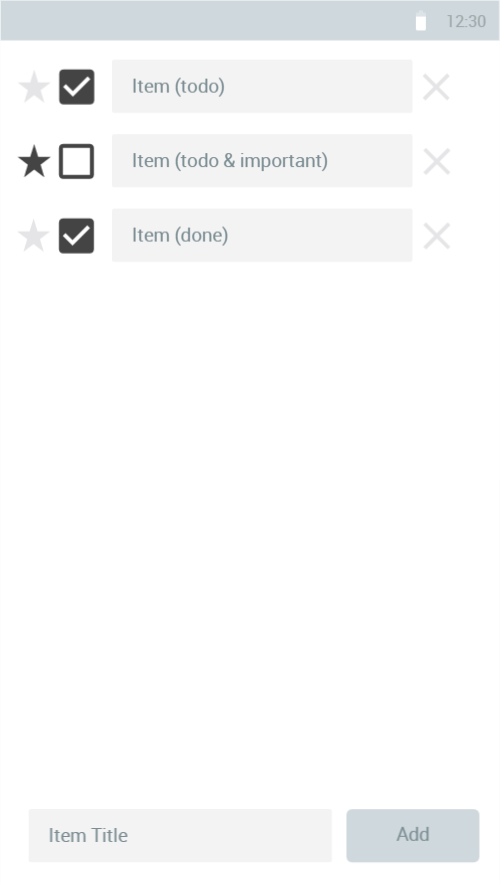
\includegraphics[scale=0.5]{img/fig/4-3-1_wireframe.png}
	\centering
	\caption{Wireframe der App}
	\label{fig:wireframe}
\end{figure}

Eine Besonderheit in der Darstellung lässt sich innerhalb der priorisierten Elemente finden. Um diese weiter hervorzuheben, werden diese an den Anfang der Liste gesetzt. Es entstehen somit zwei Teillisten, welche sich jedoch in derselben Listenansicht befinden. Wird nun ein zuvor nicht-priorisierter Eintrag priorisiert, so wechselt dieser seine Position ans Ende der Liste mit den bereits priorisierten Einträgen (bzw. wird oberhalb der ersten nicht-priorisierten Elements platziert). Alle Einträge zwischen der alten und der neuen Position des gerade betrachteten Eintrags werden um eine Listenposition nach unten verschoben. Bei Entfernen der Priorisierung wird das entsprechende Element nun nicht an seine ursprüngliche Position vor der Priorisierung, sondern an den Anfang der nicht-priorisierten Liste verschoben. Entfernt man also bspw. die Priorisierung des letzten Elements in der priorisierten Liste, ändert sich die Reihenfolge nicht. Dieses Verhalten kann vereinfacht in der untenstehenden Abbildung dargestellt werden.

Grundsätzlich werden alle Einträge in der Reihenfolge dargestellt, wie sie angelegt wurden, mit den eben beschriebenen Ausnahmen.

Um ebenfalls für farbliche Konsistenz zu sorgen, werden die beschriebenen Elemente auf Basis der folgenden Tabelle in ihrem Erscheinungsbild konfiguriert:

\begin{table}[h!]
	\centering
	\begin{tabular}{ |c|c|c|}
		\hline
		\textbf{Bezeichnung} & \textbf{Hex-Code} & \textbf{Darstellung}\\
		\hline
		
		
		\hline
		\multicolumn{3}{|c|}{\textbf{Allgemeines}}\\
		\hline
		Hintergrund & \texttt{\#F2F2F2} &\cellcolor[HTML]{F2F2F2}\\
		\hline
		Schriftfarbe & \texttt{\#8C8C8C} &\cellcolor[HTML]{8C8C8C}\\
		\hline
		
		
		\hline
		\multicolumn{3}{|c|}{\textbf{Bedienelemente}}\\
		\hline
		Hintergrund für inaktive Bedienelemente & \texttt{\#CECECE} &\cellcolor[HTML]{CECECE}\\
		\hline
		Hintergrund der Checkbox (angewählt) & \texttt{\#1A66FF} &\cellcolor[HTML]{1A66FF}\\
		\hline
		Schriftfarbe der Checkbox (angewählt) & \texttt{\#FFFFFF} &\cellcolor[HTML]{FFFFFF}\\
		\hline
	\end{tabular}
	\caption{Farbtabelle} \label{tab:farbtabelle}
\end{table}


\section{Nutzungszyklus} \label{sec:3-nutzungszyklus}
Der Nutzer öffnet die Anwendung. Beim Laden der Ansicht wird eine Datenbank-Funktion ausgeführt, um bereits existierende Einträge zu laden und ihre entsprechenden Beschreibungen samt weiteren Attributen in die einzelnen Zellen der Listenansicht zu laden. 

Der Nutzer möchte einen neuen To-Do-Eintrag erstellen. Dafür wird ein beschreibender Text in das Texteingabefeld am unteren Rand der Ansicht geschrieben. Um einen neuen Eintrag zu erstellen, wird ein beschreibender Text in das Texteingabefeld am unteren Rand der Ansicht geschrieben. Mit der Bestätigung über den \texttt{+}-Button wird ein neuer Eintrag in die Datenbank aufgefordert, wobei das \texttt{text}-Attribut mit dem zuvor gewählten Text aus dem Eingabefeld gefüllt wird. Die Zeichenfolge der \texttt{id} wird automatisch und zufallsbasiert generiert, \texttt{done} sowie \texttt{priority} standardmäßig auf \texttt{false} gesetzt. Der neue Eintrag wird unter den bereits vorhandenen Einträgen angefügt. Stern- sowie Häkchen-Symbol werden lediglich über ihre Kontur kenntlich gemacht.

Der Nutzer möchte den Test eines Eintrages ändern. Durch direktes Tippen auf den dargestellten Text in einer Zelle wird dies ermöglicht. Es erscheint ein Cursor, welcher ebenfalls Tastatur- und Berührgesten innerhalb dieses Feldes ermöglicht. Nach bestätigter Änderung über das Verlassen des Textfeldes (d.\ h. dem Tippen auf eine andere Stelle innerhalb der Ansicht) wird erneut eine Datenbank-Funktion ausgeführt. Diese bekommt das \texttt{ToDo}-Objekt übergeben und ersetzt den bestehenden Inhalt des \texttt{text}-Attributes mit dem nun geänderten.

Der Nutzer möchte den zuvor erstellten Eintrag priorisieren. Tippt dieser auf das Stern-Symbol, wird dieses mit der zuvor definierten Farbe gefüllt. Gleichzeitig bewegt sich das priorisierte Element an das Ende der Teilliste mit priorisierten Einträgen. Eine Datenbank-Funktion wird aufgerufen, welche den \texttt{priority}-Wert des übergebenen Objekts von \texttt{false} auf \texttt{true} setzt.

Der Nutzer möchte den zuvor priorisierten Eintrag als abgeschlossen markieren. Tippt dieser auf das Häkchen-Symbol wird dieses mit der zuvor definierten Farbe gefüllt. Eine Datenbank-Funktion wird aufgerufen, welche den \texttt{done}-Wert des übergebenen Objekts von \texttt{false} auf \texttt{true} setzt.

Der Nutzer möchte den zuvor als abgeschlossenen Eintrag aus der Liste der priorisierten Einträge entfernen. Tippt dieser auf das Stern-Symbol, wird dessen Füllung entfernt. Gleichzeitig bewegt sich das Element an den Anfang der Teilliste mit nicht-priorisierten Einträgen. Die zuvor ausgeführte Datenbank-Funktion wird erneut aufgerufen, welche den \texttt{priority}-Wert des übergebenen Objekts von \texttt{true} nun wieder auf \texttt{false} setzt.

Der Nutzer möchte den Eintrag abschließend entfernen. Tipps dieser auf das Kreuz-Symbol, wird der Eintrag aus der Liste entfernt. Die Elemente unterhalb des gelöschten Eintrags verschieben sich um jeweils eine Position nach oben. Eine Datenbank-Funktion wird aufgerufen, welche das übergebene Objekt des Eintrages aus der Datenbank entfernt.

		
	\chapter{Implementierung}
		\label{chap:implementierung}
		\section{Implementierung der nativen Anwendung} \label{sec:5-ios}
Die Entwicklung der nativen Mobilanwendung wird im Folgenden exemplarisch anhand einer \textit{iOS}-Applikation dargestellt. Diese werden ausschließlich auf Mobilgeräten vom U.S.-amerikanischen Hersteller \textit{Apple, Inc.} ausgeführt, funktionieren also auf diversen \textit{iPhone}-, \textit{iPod touch}- und in gewisser Hinsicht auch auf \textit{iPad}-Geräten. Letztere sind wegen der im September 2019 in Kraft getretenen Einführung des sog. \textit{iPadOS} nicht mehr auf reine iOS-Anwendungen ausgelegt, sondern nutzen diese lediglich in Form einer Vergrößerung der Kleingeräteanwendung.

Dieses Kapitel stellt im Folgenden den gesamten Entwicklungsprozess der To-Do-Anwendung dar, welche von der Wahl der Programmiersprache und -umgebung bis hin zur Ausführung auf verschiedenen kompatiblen Geräten reicht.

Der in Sektion 2.? angesprochene Standard heutiger iOS-Entwicklung wird auch in der Praxis dieser Untersuchung angewandt. Somit fällt die Wahl der Programmiersprache auf Apple Swift 5 unter der \acs{ide} Xcode 11. Im Hinblick auf die To-Do-Anwendung, welche einen persistenten Speicher benötigt, kann hier bereits die Integration der internen Bibliothek \textit{Core Data} hinzugefügt werden.

Grundsätzlich ist es sinnvoll, mit der Gestaltung der visuellen Ansicht zu beginnen, da die erstellten Komponenten im Nachhinein explizit im Quellcode referenziert werden können, um ihnen Funktionalität zu verleihen.

\subsection{Gestaltung des \acl{ui}}
\subsubsection{Einbinden von \ac{ui}-Komponenten}
Initial beinhaltet das \texttt{Main.storyboard} eine Ansicht, welche bereits mit dem automatisch generierten \texttt{ViewController} verknüpft ist. Diese muss nun mit den in Kapitel 3 beschriebenen Komponenten gefüllt werden. Die Listenansicht wird über einen \texttt{UITableView} realisiert. Dieser füllt einen großen Teil der Ansicht aus. Der untere Rand der Ansicht wird mit einem \texttt{UITextField} sowie mit einem \texttt{UIButton} versehen, welcher als \texttt{+}-Symbol konfiguriert wird. Somit ist die hierarchisch höchste Stufe der Ansicht fertiggestellt.

Bislang existiert noch keine Konfiguration der unteren Hierarchiestufe, welche aus den einzelnen Zellen des \texttt{UITableView} besteht. Da diese dem gleichen Aufbau folgen sollen, ist die Definition \textit{einer} \texttt{UITableViewCell} genügend, sodass diese dann für die gesamte Liste verwendet und repliziert werden kann. Diese Zelle beinhaltet erneut ein \texttt{UITextField}, sowie drei \texttt{UIButton}s, welche jeweils mit einem Kreuz-, Häkchen-, und Stern-Symbol konfiguriert werden.

Die Farbgebung der einzelnen Buttons wird nach Maßgabe der Farb-Definition aus Sektion 3.3.1 als \textit{Tint} der Buttons festgelegt.

Das finale \ac{ui} der To-Do-Anwendung, wie es im Interface Builder dargestellt wird, kann dem folgenden Screenshot entnommen werden.

\begin{figure}[h!]
	\centering
	\caption{\ac{ui} im Interface Builder von Xcode}
\end{figure}

\subsubsection{Relative Positionierung der Komponenten}
Apple bietet verschiedene Mobilgeräte in verschiedenen Größen an. Der Interface Builder von Xcode erlaubt die interaktive Positionierung der \ac{ui}-Komponenten jedoch nur unter Betrachtung einer spezifischen Gerätegröße. Wird diese in der Ansicht gewechselt, fällt auf, das die Positionierung der Komponenten absolut gesetzt wird und diese somit bei kleineren Geräten über den gedachten Bildschirmrand herausgehen bzw. bei größeren Geräten nicht die gesamte Bildschirmbreite ausnutzen.

In vielen Fällen schaffen sog. \textit{Auto-resizing Constraints} Abhilfe gegen dieses Problem. In diesen Kann das Verhalten einzelner Komponenten bei bestimmten Bildschirmgrößen bestimmt werden. Dieses Verhalten beschreibt die Änderung der Position sowie der Skalierung der Komponente. So soll der \texttt{UITableView} den gesamten horizontalen Bereich des Bildschirms einnehmen. Gleiches gilt für den Bereich des Textfeldes und des \texttt{+}-Buttons. Da diese jedoch in Abhängigkeit von einander stehen (d.h. das Textfeld soll immer einen bestimmten Abstand zum Button wahren; der Button soll immer einen bestimmten Abstand zum rechten Bildschirmrand wahren), müssen diese durch eine Unteransicht logisch verbunden werden. In dieser werden dann pixel- oder prozentgenaue Abstände und Änderungen definiert. Diese Unteransicht kann dann wieder über \textit{Auto-resizing Constraints} die gesamte Breite unter der Listenansicht einnehmen. So kann die App nahtlos auf verschieden großen Geräten genutzt werden, ohne dass die Positionierung aller Komponenten für alle möglichen Bildschirmgrößen manuell gesetzt werden muss.

\subsubsection{Dynamische Änderung der Komponentenposition}
Die zuvor definierte Unteransicht, welche für das Erstellen neuer To-Do-Einträge verantwortlich ist, befindet sich zunächst noch jederzeit am unteren Bildschirmrand. Tippt der Nutzer nun in das Textfeld, um einen neuen Eintrag zu erstellen, so werden Textfeld und \texttt{+}-Button von der von unten einfliegenden Tastatur überdeckt. Somit kann der Nutzer seinen Eintrag ins Textfeld nicht sehen und diesen auch nicht über Tippen auf den Button erstellen. Diese Unteransicht muss also bei Aufruf der Tastatur zusammen \textit{mit der Tastatur} verschoben werden.

Auf technischer Ebene muss eine Verschiebung der Unteransicht initiiert werden, sobald die Tastatur zu erscheinen beginnt. Gleichermaßen muss diese Verschiebung rückgängig gemacht werden, sobald die Tastatur wieder verschwindet. Es handelt sich hierbei um \textit{Event Listening} bei einem allgemeinen \ac{ui}-Komponenten, nämlich der Tastatur. Solches Event Listening ist in Swift (noch) nicht abgesehen, weswegen auf Objective-C zurückgegriffen werden muss. Die Listener, auch \textit{Observer}, die auf das Verhalten der Tastatur achten, müssen bei Start der App initialisiert und bei Schließen der App deinitialisiert werden. Sobald einer der Observer über die Änderung des Zustands der Tastatur benachrichtigt, wird die Positionsänderung aufgerufen.

Die absolute Position einer Komponente innerhalb der Ansicht kann anhand eines Koordinatensystems visualisiert werden, welches seinen Ursprung $(0; 0)$ in der oberen linken Ecke hat. Nach rechts hin wächst die $x$-Koordinate, nach unten hin wächst die $y$-Koordinate. Somit muss bei Einfliegen der Tastatur die $y$-Position der Unteransicht um gerade die Höhe der zugrunde liegenden Tastatur reduziert werden, sodass die Unteransicht sich direkt über der Tastatur befindet. Dazu wird zunächst die je nach Sprache variable Tastaturhöhe ermittelt und die $y$-Position um genau diesen Wert reduziert. Um diese Aktion rückgängig zu machen, wird eine Erhöhung der Position um diesen Wert eingeleitet, sobald der entsprechende Observer die Funktion über das Verschwinden der Tastatur benachrichtigt. Die Unteransicht wird nun nicht mehr von der Tastatur verdeckt, sondern wirkt optisch wie ein Teil von ihr, sodass diese nun genutzt werden kann, um To-Do-Einträge zu erstellen. \\\

An dieser Stelle scheint es intuitiv, die Ansicht nun zu testen. Da bislang jedoch noch keinerlei Funktionalität implementiert ist, ist es nun wichtig, Zellen erstellen zu können. Für Testzwecke könnte eine provisorische Funktionsweise entwickelt werden, welche die Zelleninformationen zunächst im Arbeitsspeicher der Anwendung speichert. Da dies jedoch im Nachhinein zu großen Abänderungen des Quellcode-Aufbaus führen kann, werden zunächst der Persistent Service und die \ac{crud}-Funktionen definiert, welche dann direkt über den \texttt{ViewController} an das \ac{ui} angebunden werden.

\subsection{Entwicklung des Persistent Service}
Wie eingangs erwähnt geschieht die Konfiguration des Datenmodells des Persistent Service über die Konfigurationsdatei \texttt{to\_do.xcdatamodeld}. Dort kann eine neue Entität \texttt{ToDo} angelegt werden, welche die in Kapitel 3 beschriebenen Attribute (\texttt{id}, \texttt{text}, \texttt{done} und \texttt{priority}) in Form ihrer spezifizierten Datentypen beinhaltet. Da keine Beziehungen zu anderen Entitäten von Bedarf sind, kann diese Entität nun als sog. \texttt{NSManagedObject} exportiert werden. Dieses ermöglicht die Nutzung der Entität als Objekt im Quellcode und stellt notwendige Funktionen für die spätere \ac{crud}-Funktionalität bereit.

Die notwendigen Komponenten des Persistent Service liegen im \texttt{AppDelegate} bereit. In diesem wird davon ausgegangen, dass mehrere Instanzen eines solchen Services genutzt werden. Da es sich im Fall der To-Do-Anwendung jedoch um einen global gleich genutzten Speicher handelt, spricht nichts dagegen, die Komponenten in eine statische Klasse \texttt{Storage} auszulagern. In dieser Klasse werden nun auch Funktionen für die verschiedenen \ac{crud}-Operationen angelegt. Auf Basis der bereits vorhandenen Funktion \texttt{saveContext()} wird die Nicht-Flüchtigkeit dieser \ac{crud}-Operationen gewährleistet.

\subsubsection{\texttt{createToDo(...)}: Anlegen von To-Do-Elementen}
Der Aufbau der Funktion, welche für das Anlegen der To-Do-Elemente innerhalb des Persistent Service zuständig ist, wird hinsichtlich des zugrunde liegenden Quellcode-Ausschnitts beschrieben.


\begin{listing}[H]
	\inputminted{Swift}{sourcecode/ios_createToDo.swift}	
	\caption{Funktion zur Erstellung von To-Do-Elementen (Swift)}
\end{listing}

Es werden die Entitätsinformationen aus der Konfiguration der Datei \texttt{to\_do.xcdatamodeld} entnommen (Z. 2), sodass ein neues Objekt nach dieser Entität erstellt und dem Speicher zugeordnet werden kann (Z. 3). Daraufhin werden die initialen Werte der einzelnen Attribute gesetzt (Z. 6--9), wobei der beschreibende Text hier direkt aus dem Funktionsparameter entnommen wird. Zuletzt wird der Kontext (vereinfacht also der Speicher) aktualisiert und das neue Objekt wird in Form einer sog. \textit{Completion} zurückgegeben (Z. 1, Z. 13). Dieses kann in einer sog. \textit{Callback}-Funktion verwendet werden, welche nach erfolgreichem Durchlaufen der Ausgangsfunktion ausgeführt wird.

\subsubsection{\texttt{loadToDos(...)}: Laden von To-Do-Elementen aus dem Speicher}
Der Aufbau der Funktion, welche für das Laden der To-Do-Elemente aus dem Persistent Service zuständig ist, wird hinsichtlich des zugrunde liegenden Quellcode-Ausschnitts beschrieben.

\begin{listing}[H]
	\inputminted{Swift}{sourcecode/ios_loadToDos.swift}	
	\caption{Funktion zum Laden von To-Do-Elementen (Swift)}
\end{listing}

Zunächst wird der Datenabgriff vorbereitet, welcher auf die zuvor exportierte Klasse der \texttt{ToDo}-Entität zugreift (Z. 2). Auf Basis dieser Anfrage (Z. 5) wird ein Array vom Datentyp \texttt{ToDo} im gleicher Completion-Form wie zuvor zurückgegeben (Z. 6). Da dieser Vorgang \textit{Exceptions} schmeißen kann, muss dieser Vorgang entsprechend kontrolliert (d.\ h. mit \textit{Error Handling} versehen) ablaufen.

\subsubsection{Bearbeiten von Attributswerten von To-Do-Elementen}
Da das \ac{ui} mehrere Bedienelemete für das Bearbeiten eines Eintrags aufweist (d.\ h. das Ändern des Textes, der Priorität sowie des Status über Abschluss der Aufgabe), müssen entsprechend viele Funktionen für das Bearbeiten dieser Eigenschaften angelegt werden. In jeder der Funktionen wird das zu bearbeitende To-Do-Objekt mitgegeben und das zu ändernde Attribut wird mit dem neuen, ebenfalls mitgegebenen, Wert überschrieben. Das abschließende Ausführen von \texttt{saveContext()} sorgt für die Konsistenz des Objekts.

\subsubsection{\texttt{deleteToDo(...)}: Löschen von To-Do-Elementen}
Das mitgegebene To-Do-Objekt wird über die Kontext-Löschfunktion entfernt und der Stand des Kontext mit \texttt{saveContext()} gespeichert.

\subsection{Entwicklung der \ac{ui}-Funktionalität}
In Abschnitt 5.1.1 sind die verschiedenen \texttt{UIButton}-Komponenten zum \ac{ui} hinzugefügt worden, besitzen bislang jedoch keinerlei Funktionalität. Durch die in 5.1.2 implementierten \ac{crud}-Funktionen ist es nun möglich, diese mit den \texttt{UIButton}s zu verknüpfen, um diese durch entsprechenden Knopfdruck auszulösen. Eine Ausnahme bildet die Funktion \texttt{loadToDos(...)} (vgl. Abs. 5.1.2.2), welche bei Initialisierung der App aufgerufen wird. Zusätzlich soll eine Folge von Abschlussoperationen durchgeführt werden, welche die Darstellung der Anwendung analog zum Zustand des Speichers korrigiert.

Im Quellcode wird die Verknüpfung über die Kombination aus sog. \texttt{IBOutlet}-Variablen und \texttt{IBAction}-Funktionen realisiert. Um die statischen Zustände der Komponenten erkennen, editieren und nutzen zu können, werden diese in Form von \texttt{IBOutlet}-Variablen den zuständigen Klassen hinzugefügt. Dies wird sich bei der Initialisierung der Anwendung zunutze gemacht, da so die Zustände der Zellenbuttons anhand der bereits vorhandenen und zu Start der Anwendung geladenen Einträge korrekt gesetzt werden können. Sollen Aktionen, wie vorhin beschrieben, durch die Komponenten ausgelöst werden (bspw., wenn ein Button angetippt wird), nutzt man \texttt{IBAction}-Funktionen, welche immer zu einer bestimmten Komponente gehören, und ihre Anweisungen ausführen, sobald der definierte Aktionszustand erreicht ist.

\subsubsection{Verknüpfung der \ac{crud}-Funktionen}

Die Funktion \texttt{createToDo(...)} soll dem globalen \texttt{+}-Button zugewiesen werden. Das Bearbeiten (d.h. als erledigt markieren resp. priorisieren) und Löschen der bereits vorhandenen Einträge wird über die Verknüpfung mit den Buttons realisiert, welche pro Zelle jeweils einmal auftauchen. Das Bearbeiten der Eintragsbeschreibung nimmt an dieser Stelle eine Sonderrolle ein. Der Text nicht als statisches \texttt{UILabel} definiert ist, welcher sonst nur indirekt editierbar wäre. Es handelt sich, genau wie beim Textfeld für die Erstellung von To-Do-Einträgen, um ein \texttt{UITextField}, welches vom Nutzer direkt angetippt werden kann, um Änderungen vorzunehmen. Dieses kann ebenfalls sog. \textit{Actions} ausführen, wenn ein bestimmter Zustand des Komponenten erreicht ist. Im Falle der individuellen Textfelder für die Eintragsbeschreibung wird die entsprechende \ac{crud}-Funktion für die Änderung und Speicherung des Textes ausgeführt, sobald die aktive Nutzung des jeweiligen Textfeldes abgeschlossen ist, sich anschaulich also kein Cursor mehr in diesem Textfeld befindet.

Während \texttt{loadToDos(...)} und \texttt{createToDo(...)} auf globaler Anwendungsebene keine variablen Auswirkungen haben, stellen die restlichen \ac{crud}-Funktionen eine interkommunikative Hürde dar. Die Ausführung der jeweiligen Funktion muss der gewünschten Zelle zugrunde liegen. Als Frage ließe sich formulieren: Wie weiß die in der Klasse \texttt{ToDoTableViewCell} definierte \ac{crud}-Funktion, auf welche der initialisierten Zellen im \texttt{ViewController} sich die Ausführung bezieht?

Konkret begründet sich die Problematik in der Tatsache, dass die Funktionen als Zellenfunktionen definiert sind, aber nur der übergeordnete \texttt{ViewController} Informationen über die Position der individuellen Zellen hält. Diese Disziplin lässt sich mit der Einführung sog. \textit{Delegates} lösen. Bei diesen handelt es sich um Protokolle, welche Funktionen für eine Klasse deklarieren, welche stellvertretend von einer anderen Klasse definiert und ausgeführt werden. Für den Fall der zugrunde liegenden To-Do-App geschieht folgendes: Das Protokoll \texttt{ToDoCellDelegate} wird definiert und in der Klasse \texttt{ToDoCell} initialisiert. Das Protokoll deklariert lediglich spezifische Funktionsnamen, welche in der Klasse \texttt{ToDoCell} bei auslösen der zuvor beschriebenen \texttt{IBAction}-Funktionen ausgeführt werden. Gleichzeitig erbt die Stellvertreter-Klasse \texttt{ViewController} von \texttt{ToDoCellDelegate} und definiert die Funktionsabläufe. Da die Funktion per Definition immer die entsprechende Zelle als Parameter mitgegeben bekommt, ist nun bekannt, um welche Zelle es sich bei Auslösen der Zellenbuttons handelt, sodass die Operationen korrekt ausgeführt werden können.

\subsubsection{Ergänzende \ac{ui}-Operationen}
Nun gilt es, das anderweitige Verhalten der App bei Auslösen der entsprechenden \texttt{IBAction}- bzw. der delegierten  Funktionen zu definieren.

Bei Öffnen der App werden die Zellen mit der durch die Funktion \texttt{loadToDos(...)} zurückgegebenen To-Do-Einträge in Form eines Arrays gefüllt. Dabei werden zunächst alle priorisierten Einträge aufgeführt, bevor die übrigen Einträge folgen. Bei der Editierung der Textbeschreibung wird die alte Beschreibung des To-Do-Eintrages trivialerweise durch die neue ersetzt. Bei Erledigung der App wird der Zustand des Häkchens als Grundlage genommen und entsprechend gesetzt. Das Löschen eines Eintrages führt zusätzlich zur Entfernung aus dem Speicher ebenfalls zu einer animierten Verschiebung aller darunterliegenden Zellen um eine Position nach oben, sobald die gelöschte Zelle optisch entfällt. Die Priorisierung der Einträge erfordert ebenfalls eine Verschiebung von Einträgen. Sobald ein zuvor nicht-priorisierter Einträg priorisiert wird, wird er an das Ende aller zuvor priorisierten (und sich somit bereits oben befindenden) Einträge geschoben. Da davon ausgegangen werden kann, dass zu Beginn der App-Nutzung die Einträge bereits korrekt sortiert wurden, wird das erste Element der Liste gesucht, welches nicht priorisiert ist. An diese Stelle gelangt nun der neu zu priorisierende Eintrag. Darüber hinaus werden alle Einträge, welche zwischen der neuen und der alten Position des nun priorisierten Eintrags liegen, um jeweils eine Zellenposition nach unten verschoben. Analog wird be Depriorisierung verfahren: Das Element wird ans Ende der priorisierten Teilliste (resp. an den Anfang der nicht-priorisierten Teilliste) geschoben. Dies bedeutet, dass die sequenzielle Priorisierung und Depriorisierung des gleichen Eintrages im zweiten Schritt keinen Positionswechsel mit sich zieht. Dies ist an der Stelle gewollt. Die Umsetzung, ein depriorisiertes Element ganz nach unten zu schieben, könnte auf gleiche Art und Weise realisiert werden.



\subsection{Umsetzung von Benachrichtigungen über unerledigte To-Do-Einträge}
Um zu verstehen, wie die Umsetzung von Benachrichtigungen (engl. \textit{Notifications}) in einer iOS-App vonstatten geht, ist es notwendig, deren Nutzungszyklus nachzuvollziehen. Nach der Installation einer Anwendung, welche Benachrichtigungen unterstützt, wird der Nutzer vom System aufgefordert, zu entscheiden, ob Benachrichtigungen der App erwünscht sind. Erst nach expliziter Bejahung dieser Frage werden diese angezeigt. Somit muss zunächst die Systemanbindung der Benachrichtigungen gewährleistet (und somit implementiert) werden, bevor diese definiert werden können.

Das Verhalten der App gegenüber dem Betriebssystem iOS nach außen wird über den \texttt{AppDelegate} gesteuert (vgl. Abs. 2.4.1.1.5). Die Umsetzung von Benachrichtigungen geschieht über die zusätzliche Funktionalität der Bibliothek \texttt{UserNotifications}. Es handelt sich in diesem Fall um lokale Benachrichtigungen, da die Anzahl der unerledigten To-Do-Einträge direkt über die sich im Speicher befindlichen Informationen erfolgen kann.

\subsubsection{Initialisierung und Genehmigung von Benachrichtigungen}
Die Bibliothek \texttt{UserNotifications} wird im \texttt{AppDelegate} importiert. Das sog. \textit{Notification Center} kann nun bei Start der Anwendung initialisiert werden. Es werden Standardeinstellungen für die Benachrichtigungen definiert, welche greifen, sobald der Nutzer diese genehmigt hat. Das Erscheinungsbild, der dazugehörige Ton und weitere Aspekte können dann im Nachhinein von Nutzer in den Systemeinstellungen angepasst werden. Bei diesen Standardeinstellungen handelt es sich zunächst um das Erscheinungsbild der Benachrichtigung, wenn die App im Vordergrund des Gerätes läuft, somit sichtbar ist. Als gewünschte Standardeinstellungen werden ein \textit{Alert} (d.h. ein darüberliegendes Fenster) sowie ein Warnton gewählt. Im Sinne der zuvor definierten Architektur ist ebenfalls gewünscht, dass der Nutzer außerhalb der Anwendung Benachrichtigungen erhalten kann (bspw. im Hauptmenü, innerhalb anderer Apps, im Stand-By-Modus, im Sperrbildschirm, etc.). Diese werden ebenfalls im \texttt{AppDelegate} definiert. In diesem Fall sollen am oberen Rand des Bildschirms sog. \textit{Badges} erscheinen, welche kenntlich machen, um welche App es sich handelt und welche Benachrichtigung diese gerade liefert.

\subsection{Definition und Auslösung von Benachrichtigungen}
Die Definition und Auslösung von Benachrichtigungen geschieht nun wieder über den \texttt{ViewController}. Somit importiert dieser ebenfalls die Bibliothek \texttt{UserNotifications}. Da, wie im vorigen Abschnitt beschrieben, Benachrichtigungen nicht erzwungen werden können, müssen sog. \textit{Notification Requests} gestellt werden. Diese überprüfen, ob Benachrichtigungen vom Nutzer gewünscht sind und lösen diese bei positiver Rückmeldung aus. Solche Requests benötigen zweierlei Parameter: Der \textit{Content} gibt den Inhalt der Benachrichtigung an. Dieser kann aus einer Varietät von Komponenten bestehen; im Falle dieser Anwendung reicht eine Textzeile, welche angibt, wie viele To-Do-Elemente noch unerledigt sind. Der \textit{Trigger} gibt an, unter welchen Umständen diese Benachrichtigung ausgeführt wird. Hier wird exemplarisch auf sich periodisch wiederholende Benachrichtigungen berufen, welche täglich um eine bestimmte Uhrzeit erscheinen, für den Fall, dass unerledigte Aufgaben existieren. Exemplarisch werden hier 09:00 Uhr, 12:00 Uhr und 15:00 Uhr gewählt. Im Sinne des \textit{Triggers} zählt hier nur die Uhrzeit; die Tatsache, ob es unerledigte Aufgaben gibt, muss separat geprüft werden.

Zunächst wird der \textit{Content} definiert, welcher einem String gleicht, der die Anzahl unerledigter Aufgaben aufzeigt. Da es sich um mehrere gleichartige Trigger handelt, können diese in einem Array gelagert und iterativ abgehandelt werden. Existieren nun unerledigte To-Do-Einträge, so werden die Trigger definiert. Diese Komponenten können dann genutzt werden, um Requests an das Notification Center zu stellen, die entsprechenden Benachrichtigungen anzuzeigen. Über das Antippen der Benachrichtigung kann dann in die To-Do-App gewechselt werden.

\subsection{Deployment im Apple App Store}
Im Rahmen dieser Studienarbeit kann der reelle Einsatz der App im Apple App Store nicht betrachtet werden, da kein kostenpflichtiges Apple Developer-Konto zur Verfügung steht. Somit wird sich hier auf allgemeine Quellen bezogen, welche die Bereitstellungs-, Wartungs- und Aktualisierungsprozesse allgemein erklären.

Möchte ein Entwickler seine App im Apple App Store veröffentlichen, müssen bestimmte Vorkehrungen getroffen werden. Dazu gehört die Erstellung eines App-Icons, die Bereitstellung eines beschreibenden Textes für die App, wie dieser in der individuellen Seite im App Store dargestellt werden soll, eine definierte Altersbegrenzung, etc. Der Entwickler sendet die App via Xcode-Schnittstelle zur Evaluation aus. Diese wird von Apple getestet, bevor sie im App Store veröffentlicht wird. Auch die Beachtung der Veröffentlichungsrichtlinien von Apple wird an dieser Stelle überprüft.

Dieser Prozess wiederholt sich bei jedem Update, welches der Entwickler publiziert. Das Aktualisieren der App auf die neueste Version ist für die Nutzer meist optional, kann vom Entwickler jedoch vorausgesetzt werden; andernfalls kann die App nicht mehr vom Nutzer aufgerufen werden. Dies lässt sich jedoch nur gewährleisten, wenn eine aktive Internetverbindung seitens des Endgerätes des Nutzers vorhanden ist. Verschwindet eine App aus dem App Store, so verbleibt diese auf dem Gerät, bis sie gelöscht wird. Danach kann sie nicht erneut heruntergeladen werden.


\section{Implementierung der \acs{pwa}} \label{sec:5-pwa}
\subsection{Einrichten der Projektumgebung}
Für die Entwicklung der \ac{pwa} wird die Entwicklungsumgebung \textit{Webstorm} von JetBrains gewählt, da sie die viele Routineaufgaben selbstständig beziehungsweise mit geringem Aufwand ausführt.

Wie für die Entwicklung der meisten modernen Webanwendungen ist die Installation der \textit{Node.js} Laufzeitumgebung notwendig. Mit dem integrierten Paketmanager \textit{npm} lassen sich Bibliotheken leicht zum Projekt hinzufügen.
Um die \textit{Angular} Anwendung automatisiert zu erstellen, ist zuerst die Installation des Angular \acf{cli} erforderlich. Mit dem Konsolenbefehl \texttt{npm install -g @angular/cli} wird npm aufgefordert, die neuste Version der Angular \ac{cli} global auf dem System zu installieren.


Mit dem Befehl \texttt{ng new todoapp} wird die Angular \ac{cli} (in der Konsole als \texttt{ng} abgekürzt) dazu gebracht, ein Angularprojekt inklusive nötiger Dateistrukturen zu erstellen.

\begin{figure}[h!]
	\centering
	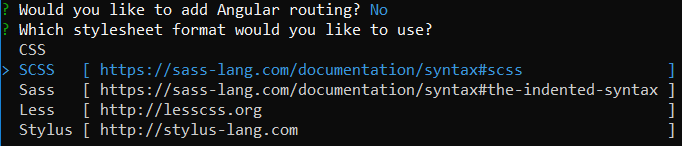
\includegraphics[width=0.58\textwidth]{img/angular_cli_css.PNG}
	\caption{Stylesheetformate beim Erstellen der Angularanwendung}
	\label{fig:stylesheet_formate_cli}
\end{figure}

Die \ac{cli} bietet dem Nutzer einige Optionen bei der Erstellung an, die jedoch in diesem Projekt nicht zwangsläufig benötigt werden, so kann beispielsweise ein Routing oder Unittesting eingerichtet werden.
Außerdem unterstützt die \ac{cli} verschiedene Stylesheetformate (siehe Abbildung \ref{fig:stylesheet_formate_cli}). Das ist für Entwickler sehr praktisch, wenn sie einen dieser CSS-Dialekte beherrschen. Die Arbeit mit Variablen in Stylesheets bevorzugt wird, werden in diesem Projekt SCSS Dateien verwendet.


\subsection{Aufbau der Anwendung mit Angular}

Im Folgenden werden die einzelnen Komponenten der \textit{Angular}-Anwendung erläutert. Es wird explizit darauf hingewiesen, dass \textbf{Quellcode-Ausschnitte teilweise stark gekürzt worden sind}, um die Lesbarkeit zu erhöhen.

\subsubsection{Bereitstellen der Klasse \texttt{TodoItem} zur Datenspeicherung}

Die Komponenten tauschen untereinander Daten aus. Damit diese einer einheitlichen Struktur folgen, wird eine Klasse \texttt{TodoItem} erstellt, die einen Todo-Eintrag repräsentiert. Objekte dieser Klasse können jetzt einfach zwischen Komponenten ausgetauscht und modifiziert werden.

\begin{listing}[h!]
	\inputminted{TypeScript}{sourcecode/pwa_todoitem_klasse.js}
	\caption{\texttt{TodoItem}-Klasse zur Datenspeicherung (gekürzt)}
	\label{sourcecode:todoitem_klasse}
\end{listing}

Wie im Ausschnitt \ref{sourcecode:todoitem_klasse} zu sehen, hat ein Todo-Element eine Aufgabenbeschreibung (Zeile 2), zwei boolesche Werte, die speichern, ob das Element als wichtig oder abgeschlossen markiert worden ist (Zeile 4 und 5) und eine eindeutige ID (Zeile 2). Die ID hilft später ein bestimmtes Todo-Element zu modifizieren.

\subsubsection{Implementierung des \texttt{todoService} für die Datenverwaltung}
Alle Todo-Einträge sollen persistent auf dem Gerät gespeichert werden. Dafür wird ein Angular-Service erstellt: der \texttt{todoService}. Er ist für die \acf{crud} Operationen zuständig.

\begin{listing}[h!]
	\inputminted{TypeScript}{sourcecode/pwa_todo_service.ts}
	\caption{Klasse \texttt{TodoService} (gekürzt)}
	\label{sourcecode:pwa_todo_service}
\end{listing}

In Ausschnitt \ref{sourcecode:pwa_todo_service} sind die Kernfunktionen des Services abgebildet. Der Service speichert ein Array von \texttt{TodoItem}-Objekten. Wenn der Nutzer ein Element hinzufügt, erstellt der Service ein neues Datenobjekt und speichert dieses im Array und dem Browserspeicher (Zeilen 16-18). Die Funktionsweise der übrigen \ac{crud}-Operationen ist analog dazu.

Mit \texttt{localStorage} (Zeilen 8-14) kann auf den\textit{ Key-Value-Store} des Browsers zugegriffen werden. Beim Speichern werden die Todo-Elemente als \ac{json}-Objekt im Store abgelegt und analog dazu geladen. Der Key-Value-Store verliert seine Daten beim schließen der Seite nicht und besitzt kein Ablaufdatum, wie ein Cookie \cite{LocalStorage}.

\begin{figure}[h!]
	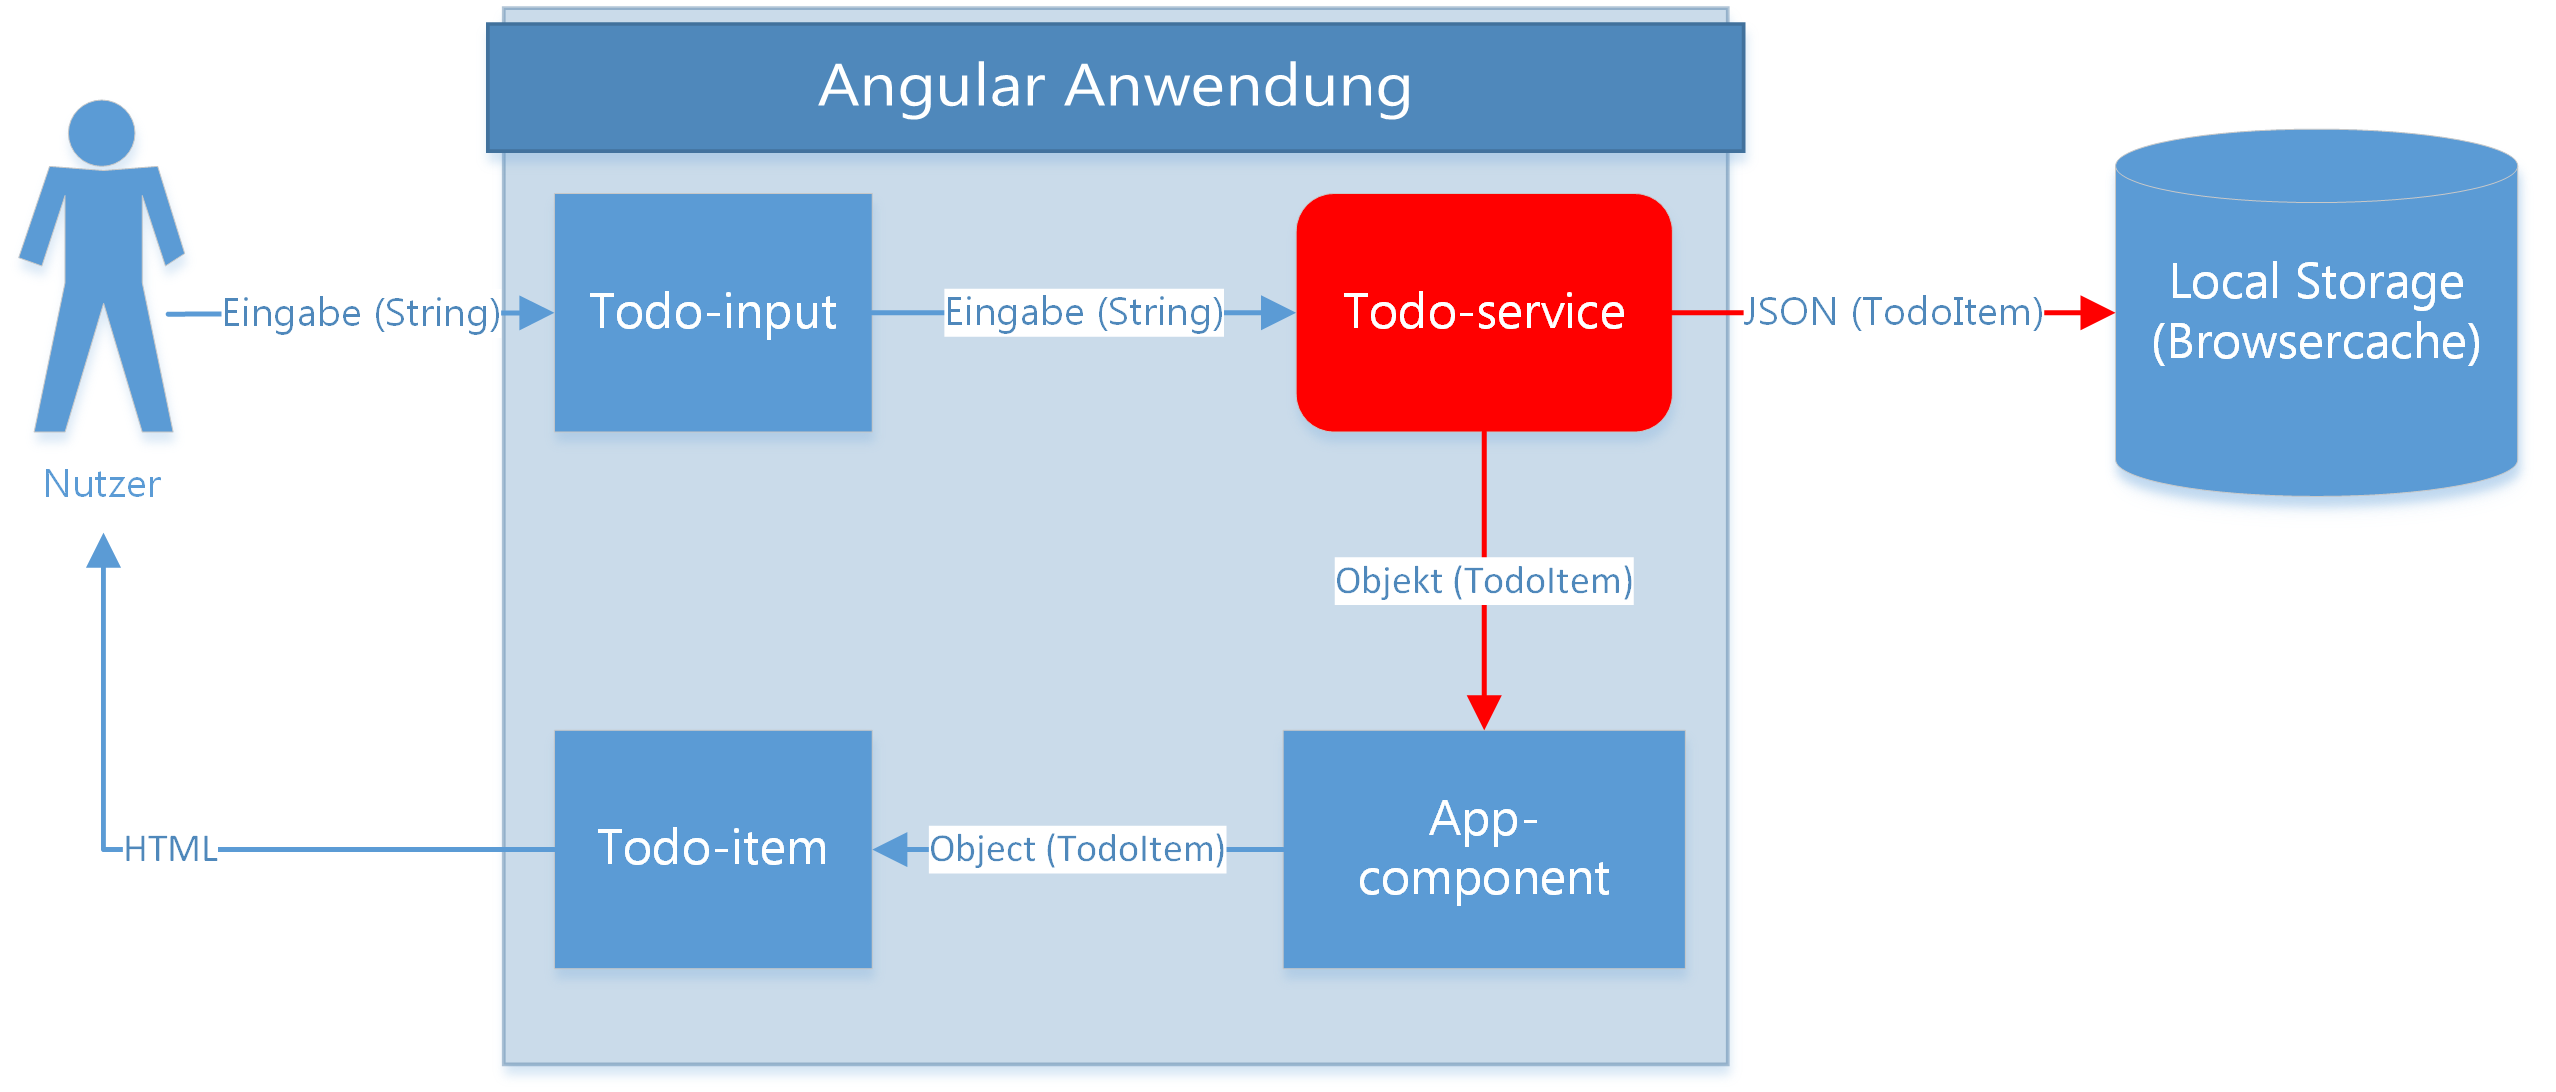
\includegraphics[width=\textwidth]{img/pwa_datenfluss_erstellen.png}
	\centering
	\caption{Datenfluss bei Erstellung eines Todo Eintrages}
	\label{fig:pwa_datenfluss_erstellen}
\end{figure}

Abbildung \ref{fig:pwa_datenfluss_erstellen} zeigt den Datenfluss beim Erstellen eines Todo-Eintrags. Die Todo-Beschreibung wird vom Nutzer über ein Eingabefeld an den Service weitergereicht. Dieser erstellt ein entsprechendes Datenobjekt und reicht es der Stammkomponente weiter, worüber schlussendlich HTML-Code erzeugt werden kann. Gleichzeitig speichert er das neue Element im Browserspeicher ab.

\subsubsection{Beschreibung der Dateistruktur und Komponenten der Angularanwendung}
Nach dem im Vorangegangenen beschrieben worden ist, wie das Projekt erstellt worden ist, wird im Folgenden detaillierter auf das erstellte \textit{Angular}-Projekt eingegangen. Angular, welches stark komponentenorientiert aufgebaut ist, zeigt sich auch in seiner Dateistruktur stark komponentenbezogen. In Abbildung \ref{fig:pwa_dateistruktur} sind die wichtigsten Dateien in einem Diagramm dargestellt.

\begin{figure}[h!]
	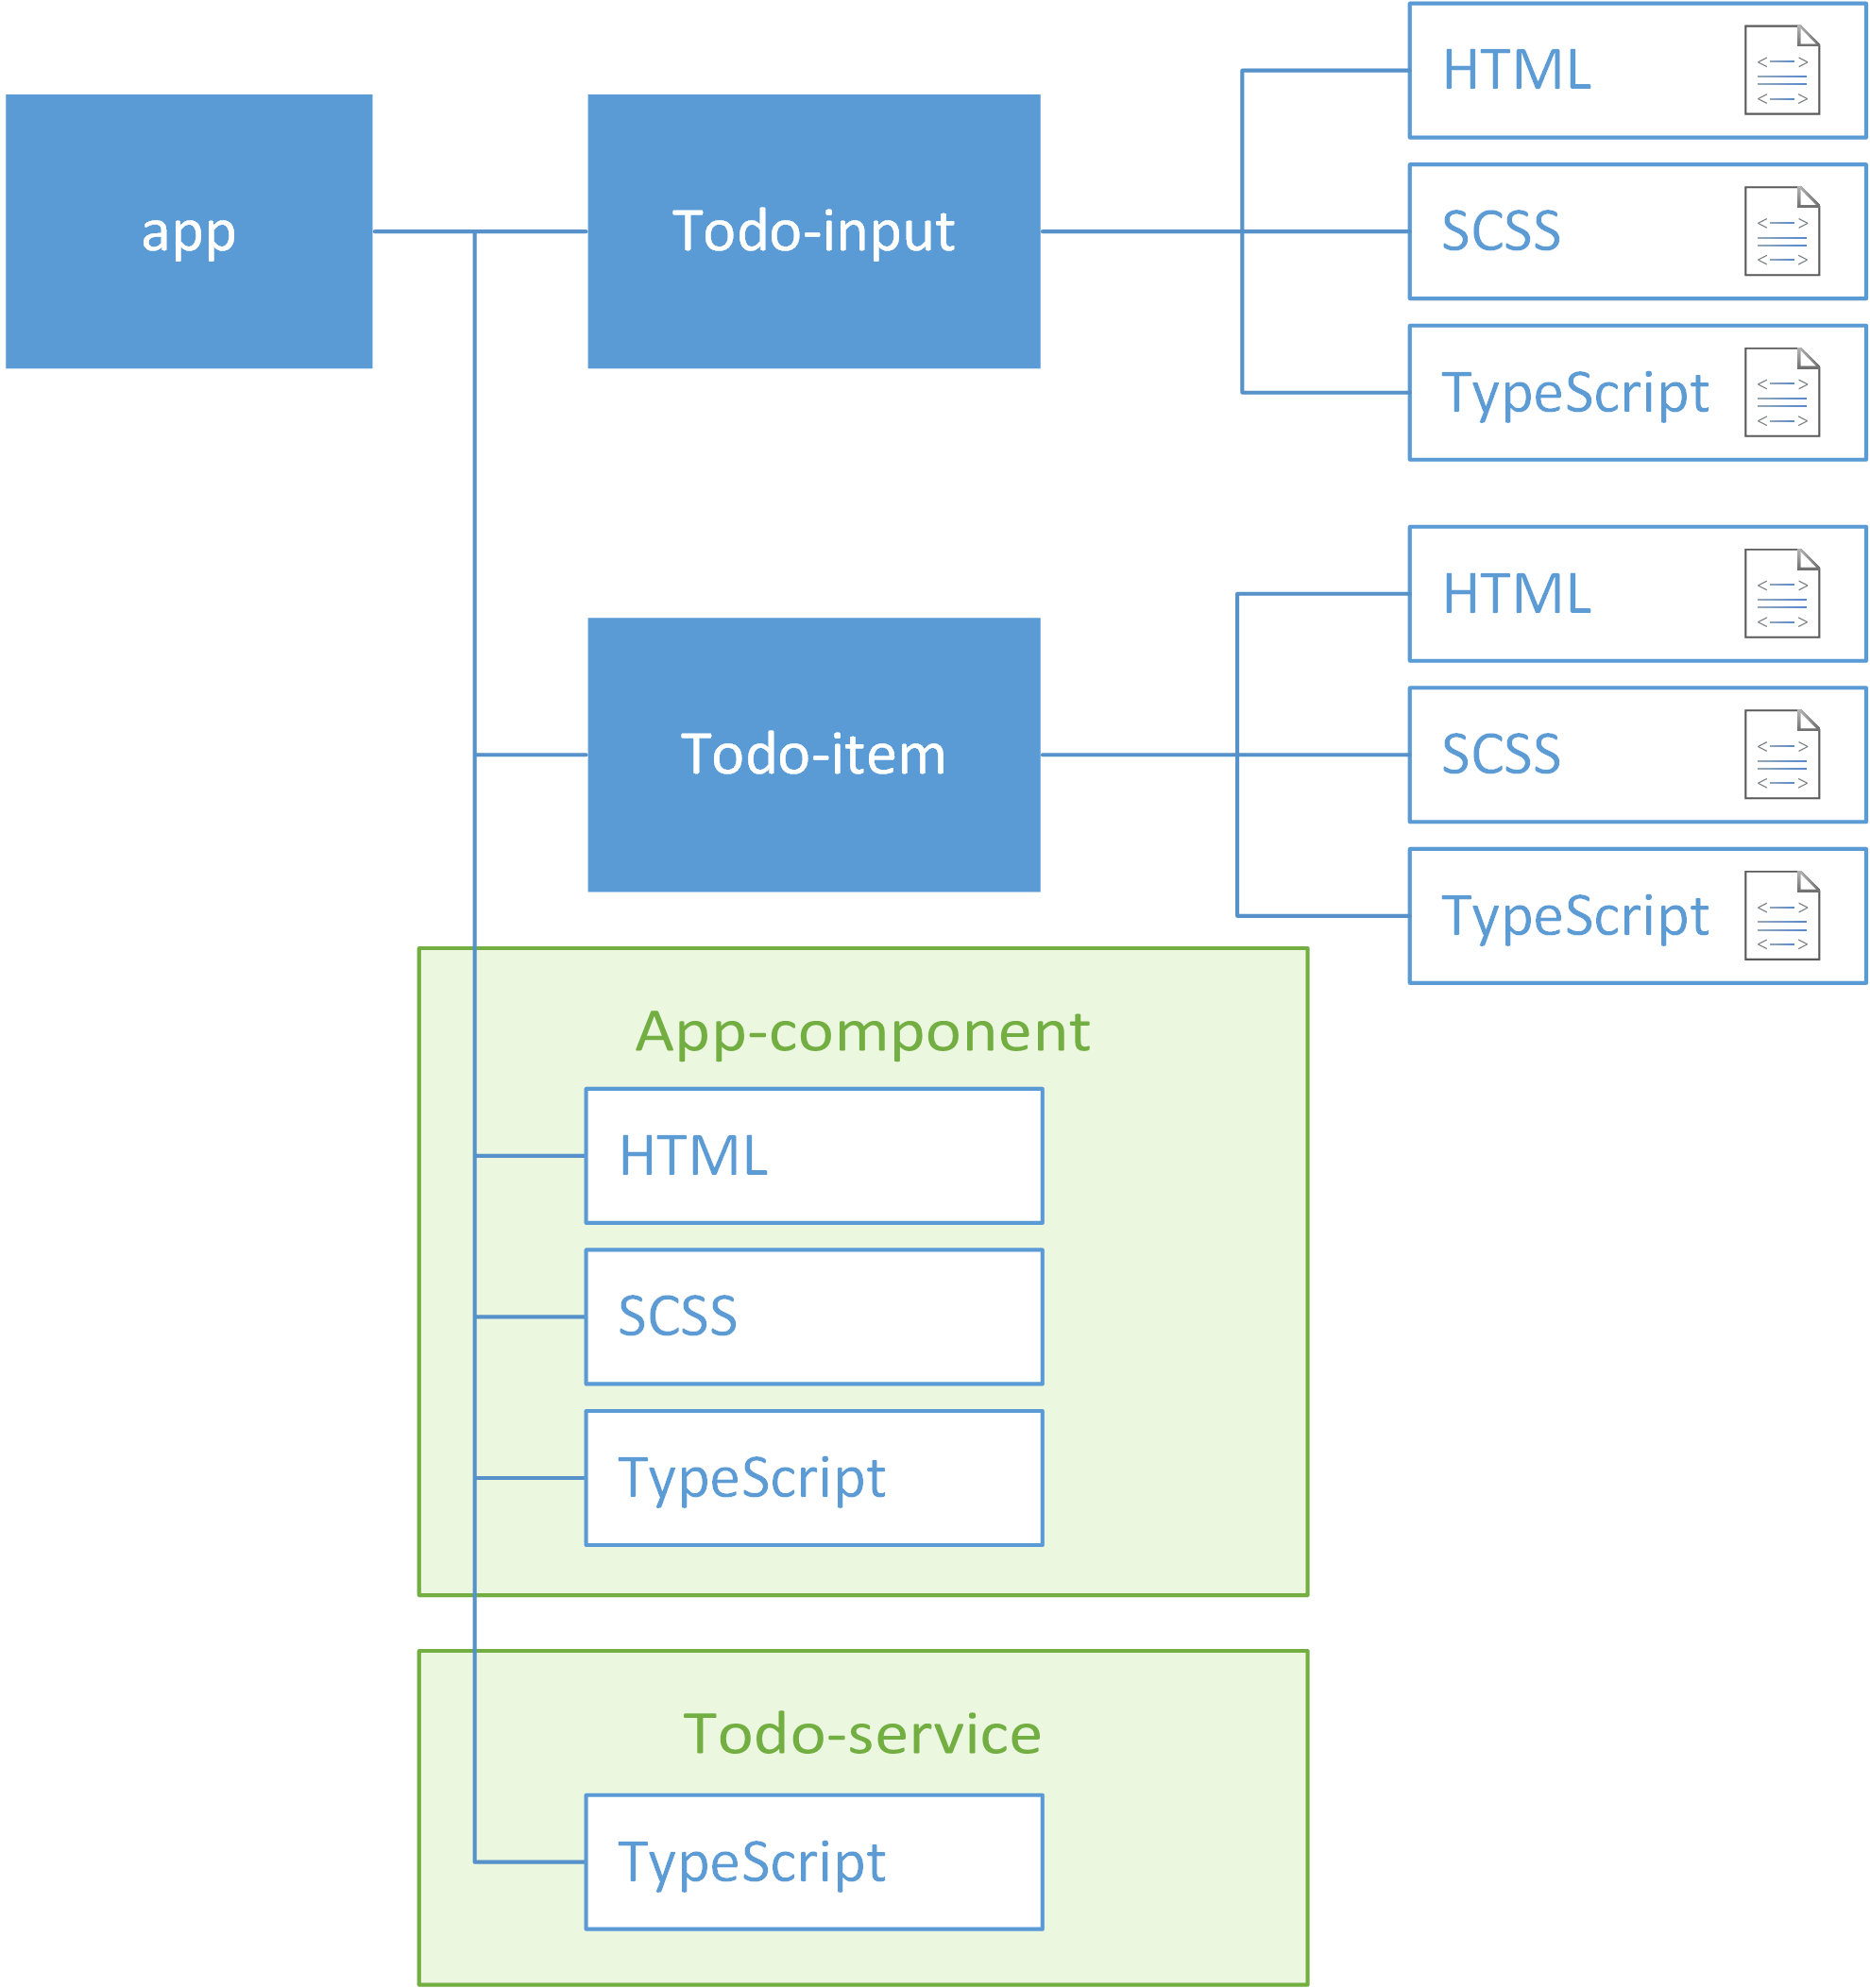
\includegraphics[width=0.6\textwidth]{img/pwa_dateistruktur.png}
	\centering
	\caption{Dateistruktur der Angularanwendung}
	\label{fig:pwa_dateistruktur}
\end{figure}

\begin{description}
	\item[Stammkomponente] Zunächst befinden sich im \texttt{app} Verzeichnis eine HTML-, eine Stylesheet- und eine TypeScript-Datei der \texttt{app-component}: die Stammkomponente. Sie dient als Container (siehe Begrifflichkeiten in Kapitel \ref{chap:grundlagen}) um die Todo-Elemente und das Inputfeld (siehe Ausschnitt \ref{sourcecode:pwa_app_component_html}, Zeile 5).
	

		
	\begin{listing}[h!]
		\inputminted{ng2}{sourcecode/pwa_app_component.html}
		\caption{HTML Template der \texttt{app-component} (gekürzt)}
		\label{sourcecode:pwa_app_component_html}
	\end{listing}

	Ausschnitt \ref{sourcecode:pwa_app_component_html}, Zeilen 1-3, zeigt, wie die Daten aus dem \texttt{todoService} in HTML-Code dargestellt werden. Wie in einer For-Schleife, wird jedes item des \texttt{todoService} einer neu erstellten \texttt{todo-item}-Komponente übergeben.
	Angular wird das HTML-Template automatisch neu rendern, wenn sich die items im \texttt{todoService} ändern.	
	
	
	\item[Todo-item] 
	Das \texttt{todo-item} ist ein einzelnes Elemente der Todo-Liste. Es enthält einen Button zum priorisieren, eine Checkbox zum abhaken des Elements, eine Textbox und einen Button zum Löschen (siehe Abbildung \ref{fig:pwa_todo_item_screenshot}).
	
	\begin{figure}[h!]
		
\includegraphics[width=0.6\textwidth]{img/pwa_todo_item.PNG}
		\centering
		\caption{Gerenderte \texttt{todo-item}-Komponente}
		\label{fig:pwa_todo_item_screenshot}
	\end{figure}
	
	
	Es ist sinnvoll jedes Listenelement in einer mehrfach instanziierten Komponente zu repräsentieren. Dies kapselt die Daten des Listenelements und die Kommunikation mit dem \texttt{todoService} von anderen Listenelementen ab. Wie bereits erwähnt bekommt jede \texttt{todo-item}-Komponente genau ein Objekt der Klasse \texttt{TodoItem} übergeben.
	
	\begin{listing}[h!]
		\inputminted{ng2}{sourcecode/pwa_todo_item.html}
		\caption{HTML Template der \texttt{todo-item} (gekürzt)}
		\label{sourcecode:pwa_todo_item_html}
	\end{listing}

	Ausschnitt \ref{sourcecode:pwa_todo_item_html} zeigt das HTML-Template des \texttt{todo-item}. Die ersten drei Input-Elemente werden durch \texttt{[(ngModel)]} mit einer Property des \texttt{TodoItem}s verknüpft, welche in der \texttt{todo-item}-Komponente gespeicht wird. Dies bewirkt folgenden Mechanismus: Wird das Input-Element verändert, ändert sich auch das gespeicherte \texttt{TodoItem}. Würde das \texttt{TodoItem} im Code modifiziert, ändert aktualisiert sich das Input-Element entsprechend.
	
	Um modifizierte Daten auch in der Datenquelle zu speichern, wird das modifizierte \texttt{TodoItem} bei jeder Änderung dem \texttt{todoService} übergeben.
	
	
	
\end{description}

\subsubsection{Kommunikation der Komponenten mit dem \texttt{todoService}}
\begin{figure}[h!]
	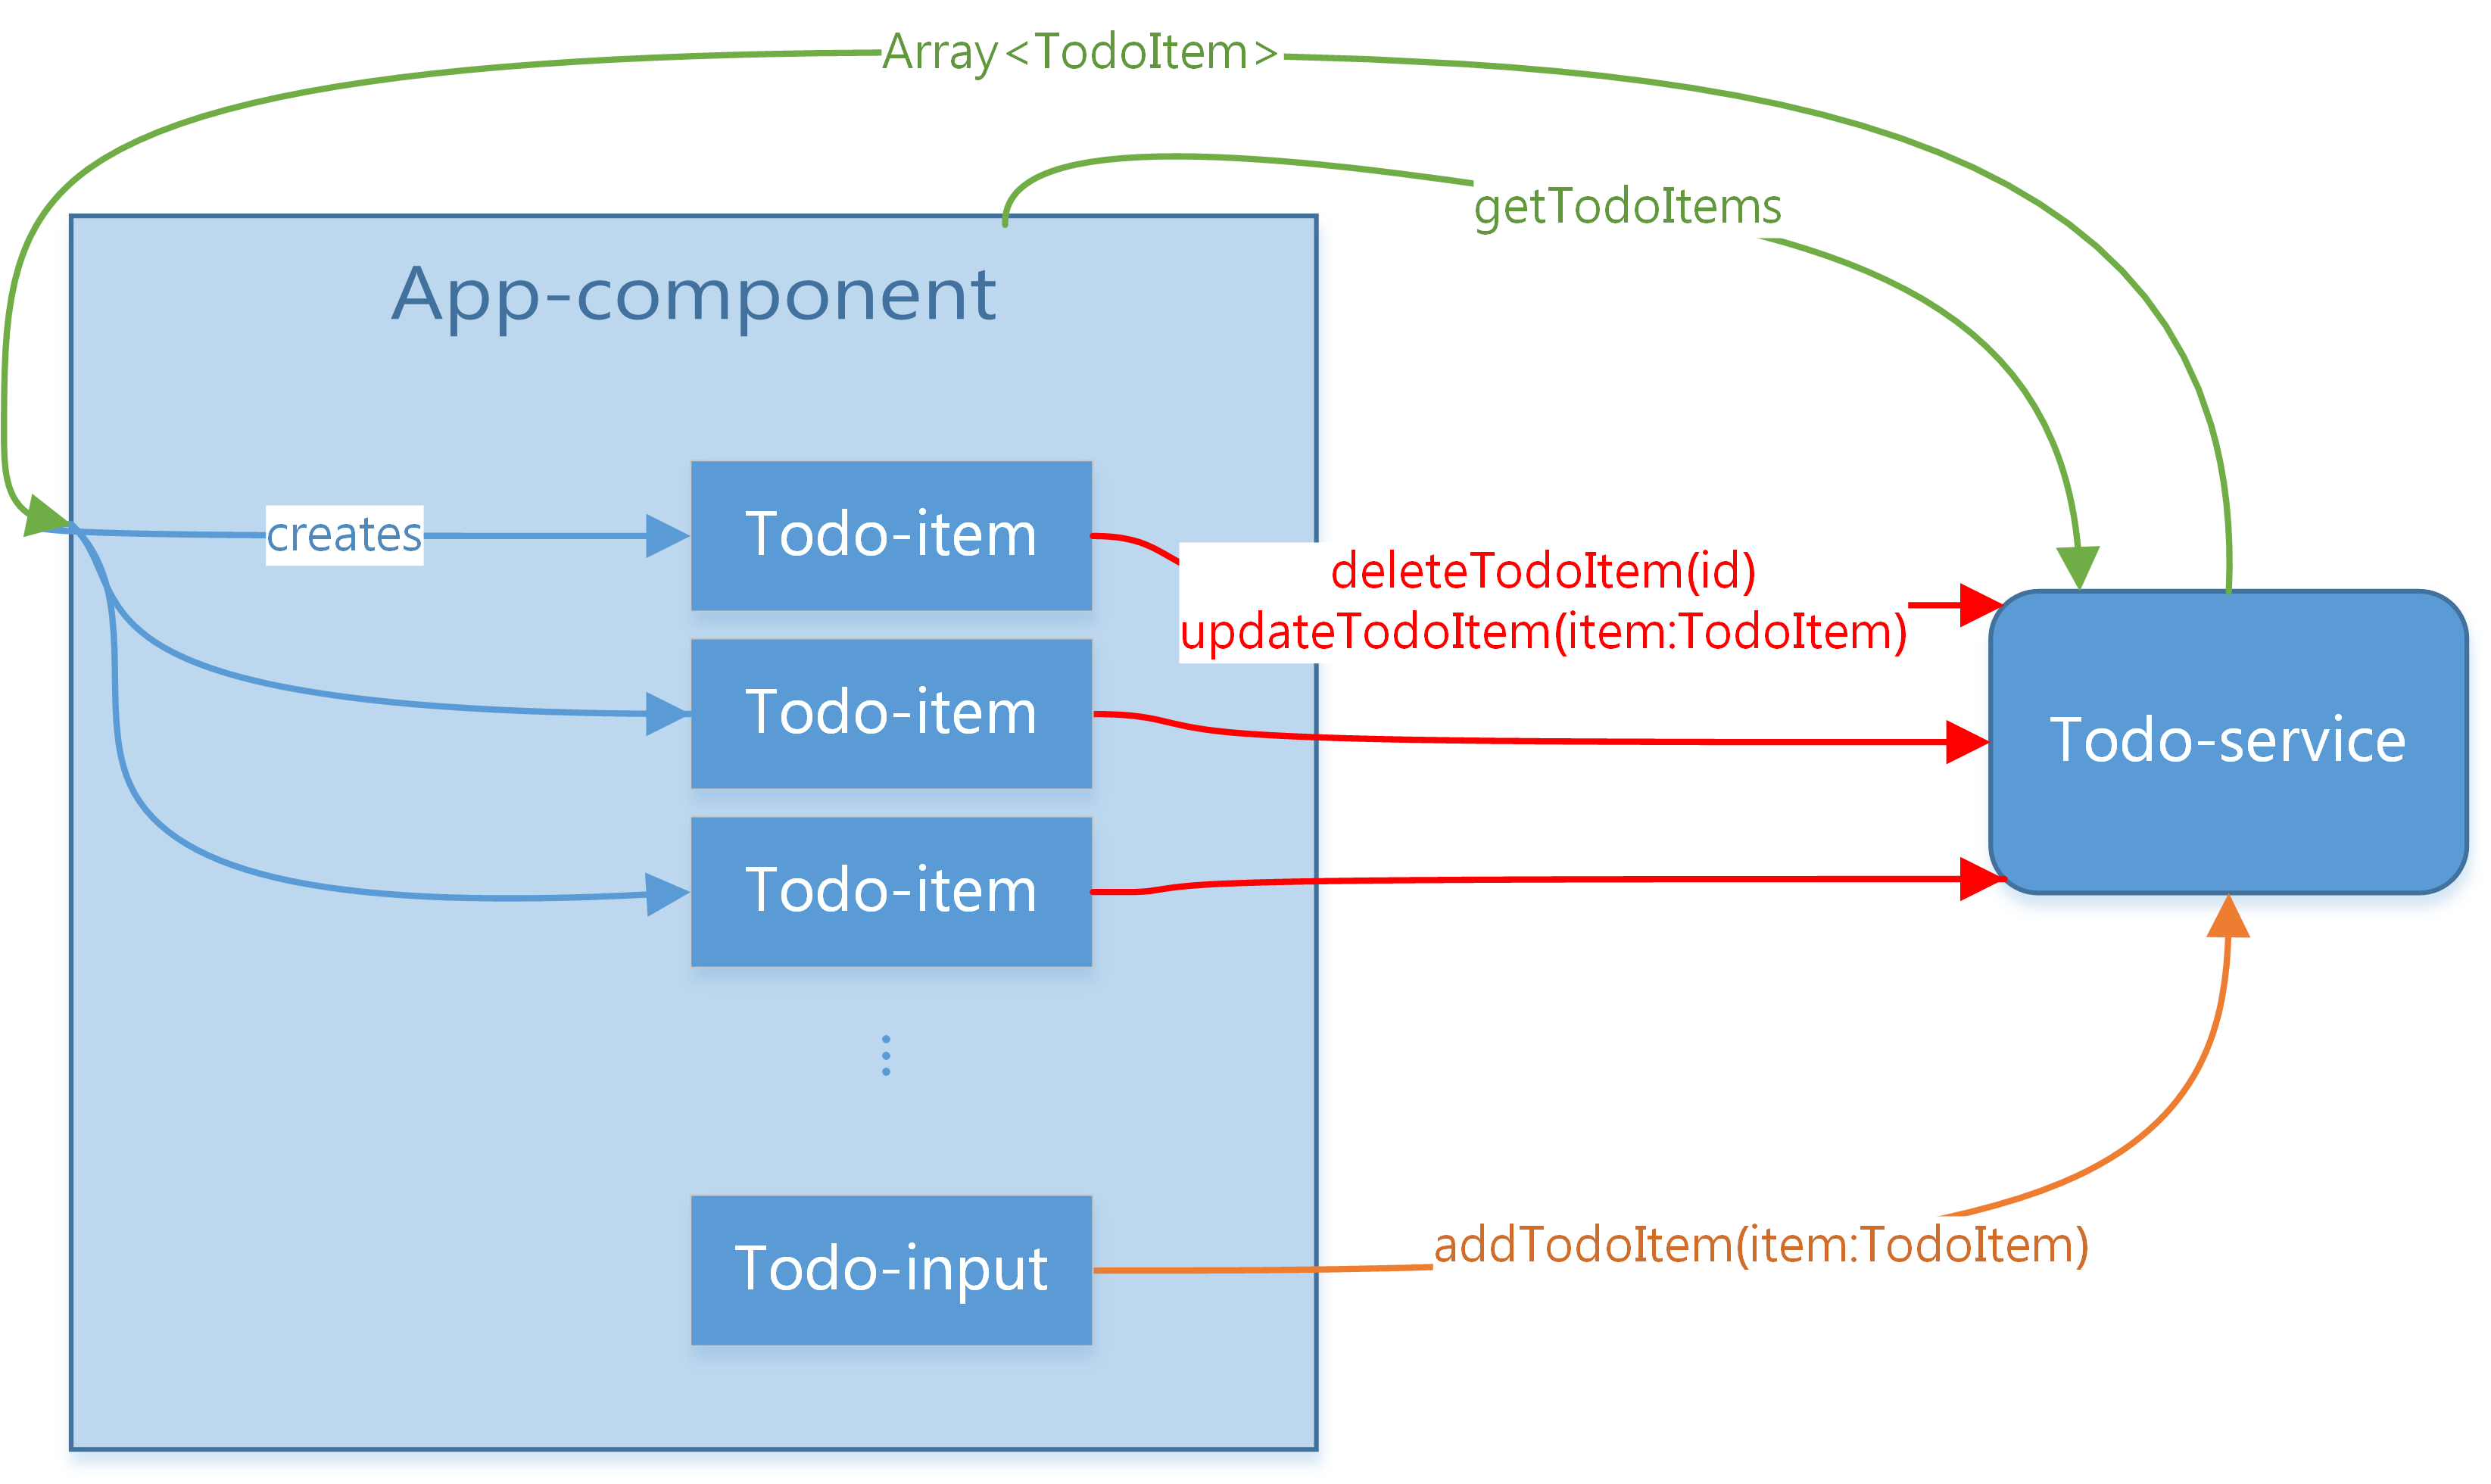
\includegraphics[width=\textwidth]{img/pwa_components.png}
	\centering
	\caption{Interaktion des Todo-service mit den Komponenten}
	\label{fig:pwa_todo_service}
\end{figure}

Abbildung \ref{fig:pwa_todo_service} fasst die Architektur der Angular-Anwendung zusammen. Den zentralen Punkt der Anwendung bildet der \texttt{TodoService}. 

Grün dargestellt ist der Datenfluss der gespeicherten Todo-Elemente zwischen der Stammkomponente und dem \texttt{TodoService}. Die Stammkomponente erhält ein Array aus \texttt{TodoItem}s und wird von Angular automatisch aktualisiert, wenn dieses sich ändert.
Die Stammkomponente erstellt für jedes \texttt{TodoItem} eine \texttt{TodoItem}-Komponente (blau dargestellt), die so als Listeneintrag sichtbar wird.

Orange dargestellt ist das Einfügen von Daten durch den Nutzer im Inputfeld der App. Der Input stellt dem \texttt{TodoService} ein neues \texttt{TodoItem}-Objekt bereit.

Rot dargestellt ist das Löschen oder Updaten von Items. Wird der Button zum Entfernen gedrückt, oder ändert sich das gespeicherte \texttt{TodoItem}-Objekt der \texttt{TodoItem}-Komponente, werden die Änderungen dem \texttt{TodoService} weitergegeben.
Für das Löschen reicht allerdings die einzigartige ID des Objekts aus.

\subsubsection{Gestaltung des \acl{ui}}
Das Styling des von Angular erzeugten HTML-Codes wird erfolgt mittels CSS. In den bereits erwähnten CSS-Dateien wird den einzelnen Elementen ein Style hinzugefügt.
Erwähnenswert ist dabei, dass alle Anforderungen im Code einzeln beschrieben werden müssen, d.h. Schriftart, Position, Farbe etc. sind einzeln zu deklarieren.

Mit der Nutzung der CSS Eigenschaft Flexbox lassen sich Elemente responsiv gestalten. Die Nutzung eines CSS oder UI-Framworks würde diese Aufgabe in einem größeren Projekt erleichtern. Mit bekannten Frameworks wie beispielsweise Material-UI lassen sich Elemente dem Material Design Prinzip anpassen (vgl. \cite{MaterialUI}), dass auf ähnliche Weise auch bei Android genutzt wird. Hierzu existieren eine Vielzahl von Frameworks mit eigenen Designphilosophien, auf die in dieser Arbeit nicht weiter eingegangen wird.

\begin{figure}[h!]
	\centering
	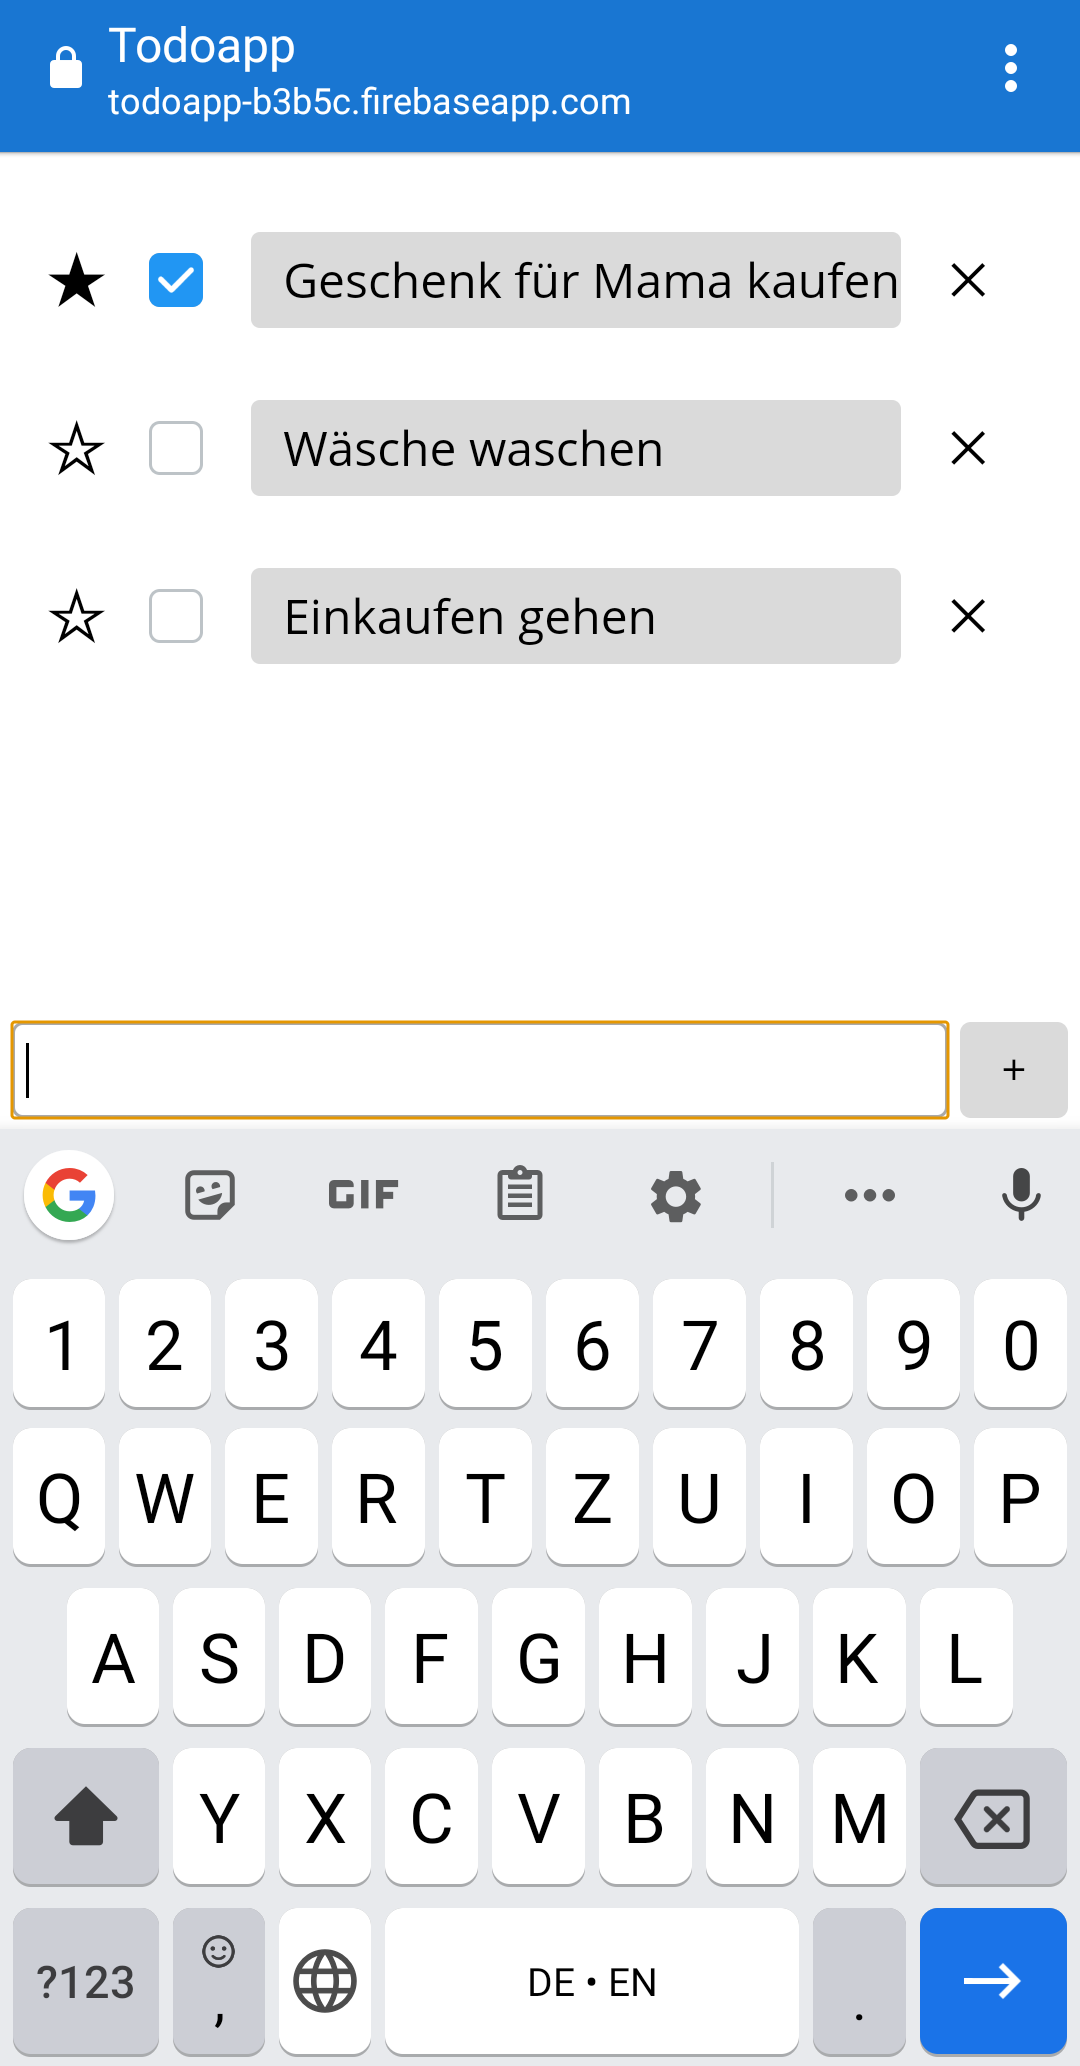
\includegraphics[width=0.4\textwidth]{img/pwa_screenshot_mit_tastatur.png}
	\caption{Screenshot der \ac{pwa} mit geöffneter Tastatur}
	\label{fig:pwa_mit_tastatur}
\end{figure}

Abbildung \ref{fig:pwa_mit_tastatur} zeigt einen Screenshot der \ac{pwa}, nachdem diese auf dem Gerät installiert wurde. Tipps der Nutzer in das Eingabefeld, öffnet sich die Tastatur und das \ac{ui} passt sich an die neuen Größenverhältnisse an.
\subsubsection{Umsetzung der Benachrichtigung über unerledigte Aufgaben}
Die definierten Anforderungen geben an, dass der Nutzer an seine Aufgaben erinnert werden soll. In der Praxis stellt sich jedoch heraus, dass die Web-Pushbenachrichtigungen über den Browser zwar sehr gut mit Webanwendungen funktionieren, aber nicht mit \ac{pwa}s ohne Internetverbindung. Mit einem Server, der zu einem bestimmten Zeitpunkt eine Nachricht an die Webanwendung schickt, ist die Umsetzung möglich, allerdings nur bei bestehender Internetverbindung. Die Anforderung wird deshalb als \textit{nicht umsetzbar} betrachtet, da das Kriterium der Offline-Verfügbarkeit nicht umgesetzt werden kann.


%\begin{figure}[h]
%	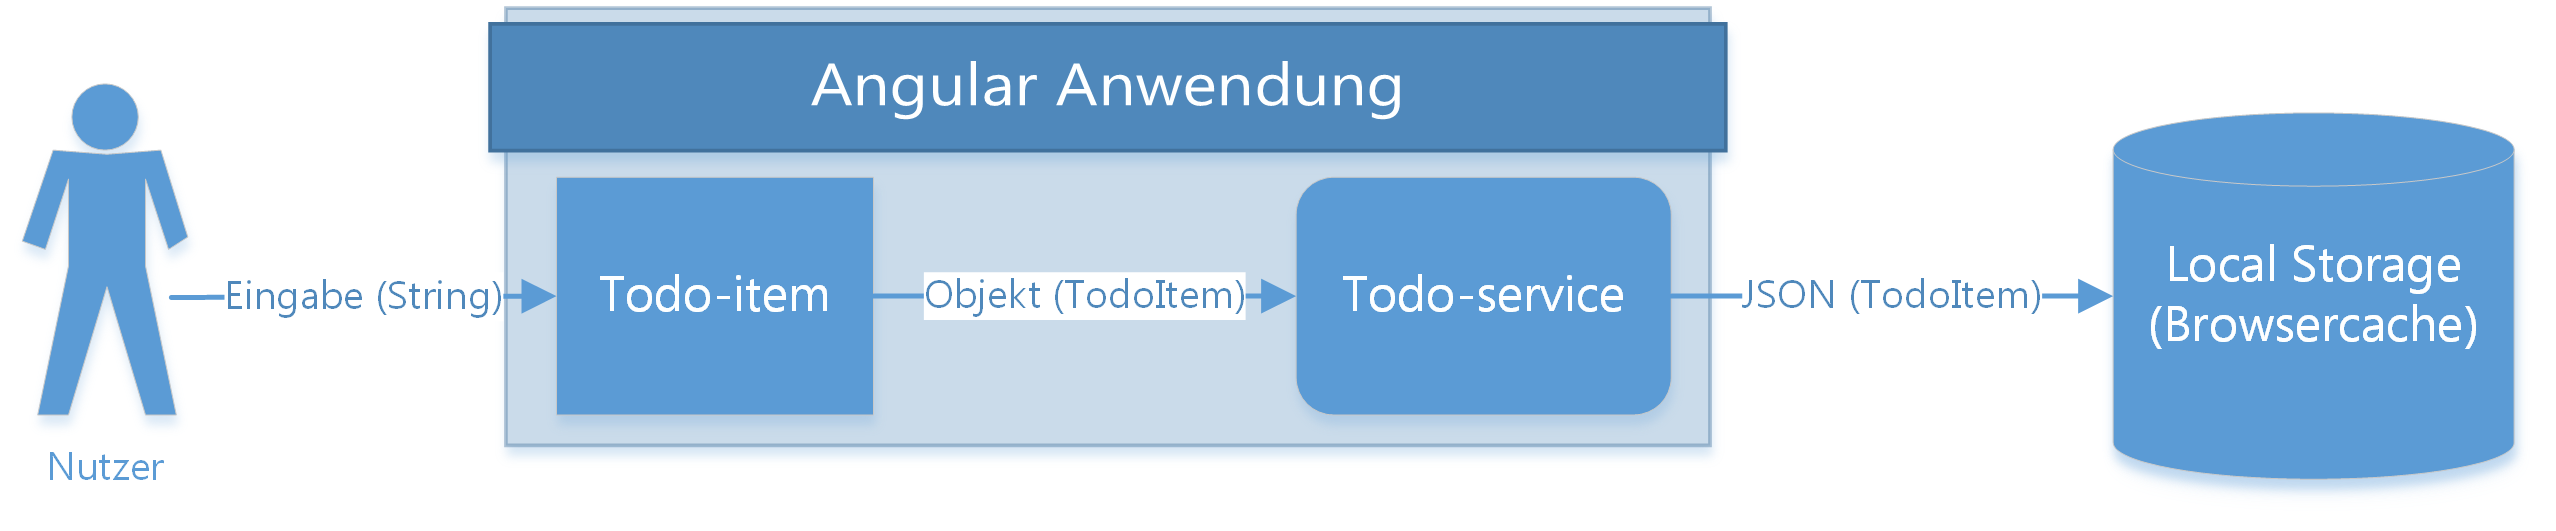
\includegraphics[width=\textwidth]{img/pwa_datenfluss_eingabe.png}
%	\centering
%	\caption{Datenfluss bei Änderung eines Todo Eintrages}
%	\label{fig:pwa_datenfluss_eingabe}
%\end{figure}

\subsection{Integration einer Manifestdatei}

Die Anwendung funktioniert zwar bereits im Browser, ist bislang aber noch keine Progressive Web App. Um dem Projekt ein \textit{Manifest} und einen \textit{Service Worker} hinzuzufügen, kann wieder die Angular \ac{cli} verwendet werden. \texttt{ng add @angular/pwa} erzeugt die entsprechenden Dateien automatisch, fügt eine manifest.json hinzu und bindet diese in die index.html Datei des Projekts ein.

Es ist festzuhalten, dass das hinzufügen der \ac{pwa}-Funktionalität keinen nennenswerten Aufwand mit sich bringt, wenn das Ziel ausschließlich die Installation der Webapp ist.

\subsection{Hosting der App mit Firebase}
Damit die \ac{pwa} als solche installiert werden kann muss sie bestimmte Kriterien erfüllen (siehe Kapitel \ref{chap:grundlagen}). Darunter ist die Notwendigkeit der Bereitstellung über \ac{https}. Dies gestaltet sich in der Praxis als schwierig, da der Angular Entwicklungsserver zwar auf \ac{https} konfiguriert werden kann, jedoch selbstsignierte SSL Zertifikate nicht aktzeptiert werden: Die \ac{pwa} kann nicht installiert werden. Für die Entwicklung ist das natürlich problematisch, so dass eine Lösung für dieses Problem gefunden werden muss.

Für die spätere Evaluierung ist der hier verwendete Hosting-Anbieter nicht relevant. Es gibt zahlreiche Alternativen, die den Anforderungen an das Hosting der Anwendung gerecht werden. Auf diese soll hier aber nicht weiter eingegangen werden. Da das Projekt jedoch aus angeführten Gründen gehostet werden muss, wird das Hosting stellvertretend mit einem Google-Service erläutert.

Googles stellt eine schnelle und elegante Lösung zum Hosten einer Webanwendung bereit: \textit{Firebase}. Über die Firebase Console, eine Webanwendung zur Verwaltung von Firebase Projekten, kann innerhalb weniger Minuten ein Projekt inklusive Hosting erstellt werden. 



Das dem Firebase \ac{cli} können automatisiert Konfigurationsdateien für das Firebase Hosting angelegt werden. Die Schritte dazu sind ebenfalls trivial:
\begin{enumerate}
	\item \textbf{Anmeldung: \\}
	      Das \ac{cli} muss mit einem Google-Konto verknüpft werden. Dazu beim Login über das \ac{cli} ein Browserfenster mit einem Google-Login Dialog.
	\item \textbf{Initialisierung: \\}
	      Die Initialisierung über das \ac{cli} legt unter anderem eine \ac{json}-Datei zur Konfiguration des Deployments an. Hier werden Dateipfade, wie beispielsweise die Start-URL oder Dateien die deployed werden sollen, gespeichert.
	\item \textbf{Deployment: \\}
	      Über die Angular \ac{cli} wird ein sogenannter Production-Build erstellt. Dies ist eine gepackte Version der Webanwendung für den Produktivbetrieb.
	      Anschließend kann die gepackte Anwendung mit \texttt{firebase deploy} auf einem von Googles Servern bereitgestellt werden.
\end{enumerate}

Die Anwendung läuft jetzt mit einer validen \ac{https}-Verbindung und kann von Nutzern installiert werden.

Das Hosting mit Firebase löst gleichzeitig ein weitere Problem: das Testen der Anwendung auf einem Smartphone. Die von Firebase bereitgestellte URL kann jetzt einfach im mobilen Chromebrowser aufgerufen und installiert werden.

\subsection{Installation der Anwendung auf Smartphone und Desktop}
\textbf{Smartphones:}\\
Nach dem Aufrufen der URL mit dem mobilen Browser, erscheint eine Meldung zum Installieren der \ac{pwa} (siehe \ref{fig:dialog_install_pwa_mobile}).

\begin{figure}[h!]
	
\includegraphics[scale=0.5]{img/pwa_add_to_homescreen.png}
	\centering
	\caption{Browserdialog zum Installieren der \ac{pwa} als Windows Desktop App}
	\label{fig:dialog_install_pwa_mobile}
\end{figure}

\textbf{Desktop:}
\begin{figure}[h!]
	\centering
	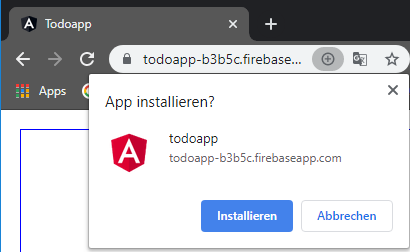
\includegraphics[width=0.48\textwidth]{img/add_to_desktop_2.PNG}
	\caption{Browserdialog zum Installieren der \ac{pwa} als Desktop App}
	\label{fig:dialog_install_pwa_desktop}
\end{figure}
In der Suchleiste von Chrome, kann der Nutzer die \ac{pwa} als Desktopanwendung installieren (siehe \ref{fig:dialog_install_pwa_desktop}).

\begin{figure}[h!]	
	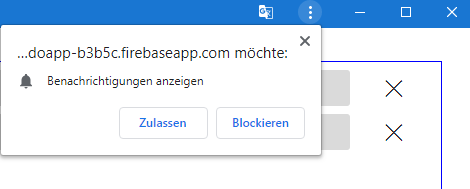
\includegraphics[width=0.48\textwidth]{img/berechtigungen_zulassen.PNG}
	\centering
	\caption{Dialog für Benachrichtigungen}
	\label{fig:pwa_benachrichtigungen_zulassen}
\end{figure}
Damit dem Nutzer Benachrichtigungen tatsächlich angezeigt werden, muss er beim erhalten der ersten Nachricht die Benachrichtigungen über einen Dialog aktivieren (siehe \ref{fig:pwa_benachrichtigungen_zulassen}).

\subsection{Update der Anwendung}

Um das Updateverhalten zu evaluieren, ist es interessant, den Updateprozess einer Webanwendung beziehungsweise \ac{pwa} zu betrachten. Um Änderungen an die Nutzer zu verteilen, muss ein Entwickler einen neuen \textit{Production Build} auf dem Server bereitstellen. Im Falle dieses Projekts werden Änderungen unter Nutzung der Firebase \ac{cli} auf den Server übertragen.

In der Praxis werden die Änderungen in der installierte \ac{pwa} nicht sofort sichtbar, wohingegen die Webanwendung beim nächsten Refresh der Seite aktualisiert wird. Dies hängt mit dem Caching der Ressourcen der \ac{pwa} zusammen. Der Service Worker lädt cachbare Dateien entweder beim Start oder nachträglich während die \ac{pwa} läuft in den lokalen Cache des Geräts.

Um dieses Verhalten zu Testen wurde ein Update mit einer auffälligen Hintergrundfarbe auf dem Server bereitgestellt. In der Desktop-\ac{pwa} war die Änderung erst nach einem Systemneustart zu sehen, wohingegen sich die \ac{pwa} unter Android nach einigen Stunden automatisch aktualisiert hatte. Dabei gab es jeweils keine Benachrichtigung zur Aktualisierung für den Nutzer.







		
	\chapter{Evaluation}
		\label{chap:evaluation}
		%===========================================================================
%	VI. Evaluation
%===========================================================================

\section{Kriterienbetrachtung}

Die zuvor definierten Vergleichskriterien finden nun Anwendung auf die entwickelten Apps. Die einzelnen Wertungen werden begründet, um zum Ende hin für die jeweilige App eine Kennzahl zu ermitteln, welche dann der Reflexion und der potenziellen Beantwortung der Forschungsfrage zugrunde liegen wird.

Es ist wichtig zu beachten, dass die exemplarische Entwicklung der nativen App innerhalb des iOS-Ökosystems nicht alleingestellt für die Gegenüberstellung zur \ac{pwa} verwendet werden kann. Bestimmte Aspekte können auf native Android-Entwicklung übertragen werden, andere werden wiederum außerhalb der Beispielanwendung begründet.

\subsection{Plattformabhängigkeit} \label{sec:6-plattform}
\textbf{Wertung native App}: $-$ \\
\textbf{Wertung \ac{pwa}}: $+$


Um das Kriterium der Plattformabhängigkeit bewerten zu können müssen die tatsächlich unterstützten Plattformen für die \ac{pwa} zuerst geprüft werden. Auf Basis des Abs. \ref{subsec:apple_ios} kann ohne weitere Betrachtung festgestellt werden, dass die Swift-Anwendung nur unter iOS und iPadOS zum Einsatz kommen kann.

\subsubsection{Browserunterstützung der \acs{pwa}}
Für Webanwendungen ist es üblich, diese mit verschiedenen Browsern zu testen. Um das Kriterium der Plattformabhängigkeit detailliert evaluieren zu können, erscheint es ebenfalls sinnvoll, die Installation der \ac{pwa} sowohl auf dem Desktop, als auch auf Android- und iOS-Smartphones zu testen.

Zum Testen der Datenpersistenz werden To-Do-Einträge angelegt und anschließend der Browser neugestartet.
Alle Browser werden mit Standardeinstellungen ausgeführt. Es werden keine Browsercaches, Cookies oder ähnliches manuell gelöscht.

\textbf{Browserunterstützung Desktop} 

\begin{table}[h!]
	\centering
	\begin{tabularx}{\textwidth}{|l||C|C|C|c|}
		\hline
		Browser              & Anwendung lauffähig & Persistente Daten & \ac{pwa} installierbar & Benachrichtigungen \\
		\hline
		Chrome 78 (64-bit)   & Ja                  & Ja                & Ja                & Ja                 \\
		Firefox 70 (64-bit)  & Ja                  & Ja                & Nein              & Ja                 \\
		Edge 41    & Ja                  & Ja                & Nein              & Nein               \\
		Internet Explorer 11 & Ja                  & Ja                & Nein              & Nein               \\
		Safari 13            & Ja                  & Ja                & Nein              & Nein               \\
		\hline
	\end{tabularx}
	\caption{Browserunterstützung Desktop} \label{tab:browser_desktop}
\end{table}

Tabelle \ref{tab:browser_desktop} veranschaulicht die Funktionalität der \ac{pwa} unter den gängigen Desktop-Browsern. Microsoft Edge und Internet Explorer zeigen den Button zum Priorisieren nicht an. Dieser enthält ein Unicode-Zeichen eines Sterns.

Microsoft Edge möchte die Zustimmung des Nutzers, um Benachrichtigungen anzuzeigen, zeigt jedoch anschließend keine Benachrichtigungen an. Internet Explorer wirft den JavaScript Fehler \texttt{'Notification' is undefined}, Benachrichtigungen sind nicht implementiert.

\textbf{Browserunterstützung Smartphone}

\begin{table}[h!]
	\centering
	\begin{tabularx}{\textwidth}{|l||C|C|C|c|}
		\hline
		Browser           & Anwendung lauffähig & Persistenz & \ac{pwa} installierbar & Benachrichtigungen \\
		\hline
		\multicolumn{5}{|c|}{Android}                                                                 \\
		\hline
		Chrome 78         & Ja                  & Ja         & Ja                & Ja                 \\
		Firefox 68        & Ja                  & Ja         & Ja                & Ja                 \\
		Edge 41 & Ja                  & Ja         & Nein              & Ja                 \\
		Opera 54          & Ja                  & Ja         & Nein              & Ja                 \\
		\hline
		\multicolumn{5}{|c|}{iOS}                                                                     \\
		\hline
		Chrome            & Ja                  & Ja         & Nein              & Nein               \\
		Safari 13         & Ja                  & Ja         & Nein              & Nein               \\
		\hline
	\end{tabularx}
	\caption{Browserunterstützung Smartphone} \label{tab:browser_smartphones}
	
\end{table}

Tabelle \ref{tab:browser_smartphones} veranschaulicht die Funktionalität der \ac{pwa} unter den mobilen Betriebssystemen und den jeweils gängigen Mobil-Browsern. Verweigert der Nutzer die Benachrichtigungen einer Webseite, ist es meist umständlich, die Berechtigung für Benachrichtigungen einer Website zurückzusetzen. Beim Browser Opera muss der Nutzer dann bpw. durch fünf Menüs nacheinander navigieren, um die deaktivierten Benachrichtigungen wieder zu aktivieren.

\subsubsection{Bewertung native App}
Die iOS-Anwendung kann nur auf einem relativ geringen Anteil der führenden Mobilgeräte verwendet werden. Anders als bei der \ac{pwa} kann auch keine limitierte Nutzung gewährleistet werden. An dieser Stelle greift auch kein Argument, welches sich auf die Exemplarität der nativen Entwicklung bezieht. Für die Nutzung verschiedener Plattformen in ihrer nativen Form müsste eine App mehrmals entwickelt werden. Diese Erkenntnis würde auch bei der Umsetzung der Beispielanwendung unter Android greifen, mit der Ausnahme, dass Android-Apps untereinenander eine deutlich höhere Geräteunabhängigkeit aufweisen, da Android von einer Vielzahl Smartphoneherstellern unterstützt wird, während iOS nur unter der eigenen Marke zur Anwendung kommt. Es existieren zwar Frameworks, welche die plattformübergreifende Entwicklung von Apps und deren native Bereitstellung in den entsprechenden Bezugspunkten erlauben (bspw. das JavaScript-Framework \textit{ReactJS}), jedoch entfällt dieses aus dem Betrachtungsrahmen dieser Arbeit. Außerdem müssten auch dort Änderungen vollzogen werden, die sich in den Unterschieden der Benutzeroberflächen der einzelnen Betriebssysteme begründen. Das Kriterium wird hier mit eher schlecht bewertet. Die Bewertung schlecht kommt nicht zum Einsatz, da die Apps in ihrem Ökosystem trotzdem ausnahmslos geräteübergreifend funktionieren.

\subsubsection{Bewertung \ac{pwa}}
Die Praxis zeigt, dass die Webanwendung zwar plattformübergreifend auf iOS, Android und Desktop funktioniert, aber nur Android-Nutzer von der Installierbarkeit der \ac{pwa} profitieren.
Hier soll ein Vergleich zur nativen iOS App geschlossen werden. Beide unterstützen die Installation auf einer mobilen Plattform, die \ac{pwa} bietet jedoch auch die Nutzung im Web für iOS-Geräte und eine installierbare Anwendung für Desktopgeräte und ist damit in diesem Kriterium der nativen App überlegen. Das Kriterium wird mit eher gut, aber nicht mit gut bewertet, da die \ac{pwa} nicht auf iOS-Mobilgeräten installiert werden kann.


\subsection{Installation} \label{sec:6-installation}
\begin{tabbing}
	mmmmmmmmmmmmm				\= \kill
	\textbf{Wertung native App}: \> $++$ \\
	\textbf{Wertung \ac{pwa}}: \> \Circle
\end{tabbing}

\subsubsection{Bewertung native App}
Folgende Erkenntnisse basieren nicht auf der Entwicklung der Beispielanwendung, können jedoch zu einem ausreichenden Grad nachvollzogen werden (vgl. Abs. \ref{subsubsec:use-ios}), um sie in die Bewertung mit einfließen zu lassen.

 Native Anwendungen werden über einen zentralen Bezugspunkt gefunden, heruntergeladen und installiert. Der Nutzer kann über Stichpunkte und Suchbegriffe nach einer Vielzahl von Apps suchen und die gewünschte Anwendung herunterladen. Homepages, welche ihre Inhalte ebenfalls in Form von nativen Apps bereitstellen, zeigen dies oft in der Mobilversion ihrer Homepage an, sodass eine direkte Verknüpfung erstellt wird. Zwar könnte als Kritikpunkt angesehen werden, dass eine Homepage direkt als \ac{pwa} bezogen werden könnte. Dafür müsste jedoch jede Homepage die Möglichkeit einer \ac{pwa}-Installation bereitstellen, was zurzeit nicht der Fall ist.
 
 Sowohl unter dem Apple App Store als auch im Play Store von Google werden Apps vor ihrer Veröffentlichung geprüft, sodass keine Probleme (vor allem im Hinblick auf die Sicherheit des Endgerätes) bei der Benutzung entstehen. Es besteht in allen Fällen eine Qualitätskontrolle, welche unvorhersehbares Verhalten der bezogenen App vermeidet.
 
 Da sich kein unentkräftbares Argument gegen die Installationskriterien finden lässt, kann dieser Prozess mit gut bewertet werden.
 
\subsubsection{Bewertung \ac{pwa}}
Die \ac{pwa} wird über den Browser installiert. Daher ist die Installation stark abhängig vom verwendeten Browsertyp. Teilweise ist die Installation der Anwendung bedingt durch den Browser überhaupt nicht möglich. Bezogen auf den Desktopbrowser Chrome dürfte es in der Praxis häufig vorkommen, dass Nutzer die Bedienelemente zur Installation im Browser nicht als solche wahrnehmen (s. Abb. \ref{fig:dialog_install_pwa_desktop}). Dies wird als negativ gewertet.

Die Installation ist für den Nutzer nicht nachvollziehbar. Er sieht nicht, dass bzw. wie viele Daten bereits heruntergeladen wurden. Der ein oder andere Nutzer wird sich möglicherweise nicht bewusst sein, dass \textit{Zum Startbildschirm hinzufügen} eine tatsächliche Installation ausführt. Die Installation dauert je nach Komplexität der Webanwendung keine ganze bis wenige Sekunden. Die Deinstallation auf Android Geräten erfolgt wie bei nativen Apps. Bei der Desktop-\ac{pwa} ist diese unter Windows sogar deutlich einfacher, als bei Desktopanwendungen.

Insgesamt ist die Installation einer \ac{pwa} sehr einfach und mit nur einem Befehl des Nutzers ausführbar. Das gilt aber nur dann, wenn der Nutzer das Konzept der \ac{pwa} begriffen hat, was nach heutigem Stand wohl nicht der Fall sein dürfte. Die Installation selbst kommt ohne Lizenzvereinbarungen oder Installationspfade daher und ist außerdem bemerkenswert schnell.

Da einige störende Punkte für den Nutzer nicht optimal sind, die Installation insgesamt aber ein einfacher Prozess ist, erhält dieses Kriterium eine neutrale Wertung.

\subsection{Speicherzugriff} \label{sec:6-speicherzugriff}
\begin{tabbing}
	mmmmmmmmmmmmm				\= \kill
	\textbf{Wertung native App}: \> $++$\\
	\textbf{Wertung \ac{pwa}}: \> $+$
\end{tabbing}

\subsubsection{Bewertung native App}
Die Beispielanwendung nutzt die Bibliothek \texttt{CoreData}, welche es erlaubt, zu speichernde Dateistrukturen in Form von Datenbank-Design anzulegen und in den Benutzungsrahmen der App hinzuzufügen. Innerhalb der Android-Entwicklung existieren verschiedene Formen app-bezogenen Speichers, welche für unterschiedliche Zwecke verwendet werden können \cite{AndroidStorage}. In beiden Fällen bedarf es \textit{Endpoints}, welche das Verhalten des Speicherzyklus definieren.

Durch eine Speicherarchitektur, welche an relationale Datenbanken erinnert, können auch komplexe Speicherstrukturen entstehen, bspw. über die Definition verschiedener Speicherareale, welche in der Beispielanwendung keinen Nutzen fanden. Anders als bei \acp{pwa} existieren keine Einschränkungen von Dateiformaten.

Das Kriterium kann somit uneingeschränkt als gut bewertet werden, da zumindest in der Beispielanwendung keinerlei Grenzen des Speicherzugriffes aufgedeckt werden konnten.


\subsubsection{Bewertung \ac{pwa}}
Die \ac{pwa} hat keinen Zugriff auf das Dateisystem. Daten werden über den Browser im Speicher abgelegt, bspw. im Key-Value-Store \texttt{local storage}. Konfigurationen und Daten können auf diese Weise einfach gespeichert werden.

Das Speichern von binären Daten, wie  bpsw. Bildern, gestaltet sich in der Praxis schwierig. Es existieren uneinheitliche, browserspezifische Lösungen. Höchstwahrscheinlich kommt der Entwickler aber nicht um das Speichern binärer Daten als kodierten Text, z.B. \texttt{Base64}.

Das Kriterium wird als eher gut bewertet, weil mit dem Browserspeicher ein Großteil der Anwendungsfälle für Datenspeicherung abgedeckt ist und diese sehr einfach von Entwicklern genutzt werden können.

\subsection{Speicherbedarf} \label{sec:6-speicherbedarf}
\begin{tabbing}
	mmmmmmmmmmmmm				\= \kill
	\textbf{Wertung native App}: \> $+$\\
	\textbf{Wertung \ac{pwa}}: \> $++$
\end{tabbing}

\subsubsection{Bewertung native App}
Nach direkter Installation der Anwendung geben die Speicherinformationen der Systemeinstellungen des Testgerätes einen Bedarf von insgesamt 475 Kilobyte an. Pro To-Do-Eintrag wächst dieser um ca. 50 Kilobyte. Es lässt sich keine genaue Schätzung für eine äquivalente Android-App ableiten, weswegen dieser Gesichtspunkt wegfällt.

Da sich die native App auf Augenhöhe mit der \ac{pwa} befindet, jedoch einen hohen Bedarfszuwachs erfordert, wenn auf den Speicher der App geschrieben wird, wird dieses Kriterium mit eher gut bewertet.

\subsubsection{Bewertung \ac{pwa}}
Die implementierte Anwendung hat einen bemerkenswert kleinen Speicherbedarf von nur 356 Kilobyte. Der belegte Speicherplatz wächst unter Android nicht messbar (\textit{App-Info unter Einstellungen}) mit Anlegen neuer To-Do-Elemente. Daher wird dieses Kriterium uneingeschränkt mit gut bewertet.

\subsection{Aktualisierbarkeit} \label{sec:6-aktualisierbarkeit}
\textbf{Wertung native App}: $+$ \\ 
\textbf{Wertung \ac{pwa}}: $++$ 

\subsubsection{Bewertung native App}
Wie auch bei der Installation administriert der zentrale Bezugspunkt (Apple App Store resp. Google Play Store) auch die Aktualisierung der auf dem Gerät installierten Apps. Je nach Nutzereinstellungen werden diese automatisch bezogen oder der Nutzer wird benachrichtigt, dass Updates verfügbar sind.

Wie bereits erwähnt werden alle Aktualisierungen, welche vom Entwickler vertrieben werden, vor Veröffentlichung erneut geprüft. Dies stellt einen Vor- wie einen Nachteil dar. Grundsätzlich kann aufgrund des Qualitätsmanagements der Bezugspunkte von einer sicheren Distribution ausgegangen werden. Andererseits können relevante Hotfixes dadurch auch verzögert werden. Sollte der Nutzer die automatischen Updates deaktiviert haben, so kann es sein, dass dieser sicherheitsrelevante Aktualisierungen nicht mitbekommt oder bewusst ignoriert, was nicht im Sinne der Entwickler ist.

Verglichen mit \acp{pwa} kann der Nutzer alle Updates genau nachverfolgen, da parallel zu diesen auch Informationen über die neuen Inhalte, Bug-Fixes, etc. veröffentlicht werden können. Sollte eine Sicherheitslücke einer neuen Version bekannt werden, so kann der Nutzer diese ignorieren, bis eine weitere Version veröffentlicht wird, welche diese behebt.

Alles in allem gewinnen gewisse Pro- bzw. Contra-Argumente an Bedeutung, je nachdem, welche Position gerade betrachtet wird. Zusammengefasst kann die Aktualisierbarkeit aber mit eher gut bewertet werden, da der Prozess an sich funktioniert und für den Nutzer in jeder Hinsicht transparent ist, jedoch unter gewissen Umständen ignoriert werden kann.

\subsubsection{Bewertung \ac{pwa}}
Der Browser bzw. der laufende Service-Worker verwaltet das Caching und die Aktualisierung der Anwendung. Der Nutzer wird über Aktualisierungen nicht informiert. Er muss ihnen nicht zustimmen und kann sie nicht vermeiden. Entwickler müssen nur die neue Version der Anwendung deployen, damit die Installationen auf den Nutzergeräten aktualisiert werden.

Da vom Nutzer keine Aktion erforderlich ist und die Aktualisierung für Entwickler sehr einfach ist, erhält dieses Kriterium die eine gute Wertung.

\subsection{Design} \label{sec:6-konsistenz-des-designs}
\begin{tabbing}
	mmmmmmmmmmmmm				\= \kill
	\textbf{Wertung native App}: \> $+$ \\
	\textbf{Wertung \ac{pwa}}: \> $-$
\end{tabbing}

\subsubsection{Bewertung native App}
Die Abhängigkeit gegenüber der geschlossenen Plattform iOS erlaubt es der Entwicklungsoberfläche und auch Apple selbst, bestimmte Richtlinien für ein konsistentes und konformes Design einzuführen und zu erzwingen \cite{AppleDesign}. Durch die Suggestion bestimmter, bereits vordefinierter, Komponenten während der Entwicklung wird dem Entwickler ein großer Teil der Gestaltungsarbeit abgenommen. Animationen, der vordefinierte Aufbau komplexer Komponenten, etc., benötigen nur wenige Quellcodezeilen für die Umsetzung und können teilweise auch komplett visuell über einen Interface Builder angelegt werden. Die teils erzwungene Konsistenz lässt sich zwar positiv für das Gesamtbild werten, stellt jedoch Hürden bezüglich der Kreativität des Entwicklers dar; für den Fall, dass eigene Animationen oder Komponentenstrukturen gewünscht sind, müssen diese sehr aufwändig definiert und umgesetzt werden. Dies kommt unter der Android-Entwicklung nicht anders zur Geltung (vgl. \cite{AndroidDesign})

Die Plattformabhängigkeit erlaubt aufgrund weniger, unterschiedlicher Bildschirmgrößen eine übersichtliche Möglichkeit, die Skalierung der Komponenten auf verschiedenen Geräten dynamisch zu gestalten. Durch die Vielzahl an unterstützten Android-Geräten lässt sich interpretieren, dass sich die Einhaltung einer solchen Konsistenz dort schwieriger gestaltet.

Die Designumsetzbarkeit stellt sich v.a. im Vergleich zu \acp{pwa} deutlich aufwandsfreier dar, jedoch bringen vor allem Kreativitätshürden durch Design-Suggestionen und die evtl. komplexe Dynamisierung der Komponentenposition unter Android nicht vernachlässigbare Schwächen mit, weswegen das Kriterium insgesamt mit eher gut bewertet wird.

\subsubsection{Bewertung \ac{pwa}}
Das Aussehen der Anwendung wird maßgeblich durch die Browserengine bestimmt, welche \ac{html} und \ac{css} rendert. Es ist seither ein bekanntes Problem, dass \ac{css} von verschiedenen Browsern unterschiedlich interpretiert wird und es für viele Features keine einheitliche Unterstützung gibt \cite{MozillaHandlingCommonHTMLCSSProblems}.

Nicht zuletzt liegt es aber am Entwickler, der große Teile des Implementierungsaufwands für das Design an Frameworks und Bibliotheken abgeben kann, um ein konsistentes Design zu erzeugen.  Schließlich gibt es Webanwendungen und Designanforderungen bereits seit einigen Jahren, sodass für die meisten trivialen Probleme bereits Lösungen bestehen.

Dieses Kriterium wird als negativ bewertet, da das Stylen mit \ac{css} zwar mit großen Freiheiten aber auch deutlichen Konsistenzproblemen einhergeht.

\subsection{Bibliotheken} \label{sec:6-bibliotheken}
\textbf{Wertung native App}: $+$ \\
\textbf{Wertung \ac{pwa}}: $++$

\subsubsection{Bewertung native App}
Apple bietet für Swift eine Vielzahl von Bibliotheken an, eine Ergänzung bieten Drittanbieterbibliotheken, welche ebenfalls in die Entwicklungsumgebung eingebunden werden können. Bei letzterem ist \textit{CocoaPods} zu nennen (vgl. \cite{CocoaPods}). Gerade die direkte Unterstützung der eigenen Bibliotheken ermöglicht eine nahtlose Inklusion in den gesamten Entwicklungszyklus. Jedoch ist JavaScript wesentlich verbreiteter als Swift, weswegen das Volumen vorhandener Bibliotheken, welche die Entwicklung vereinfachen, deutlich größer ist. Die Android-Entwicklung ist jedoch ebenfalls sehr verbreitet, weswegen gerade dafür ebenfalls eine Vielzahl von Bibliotheken zur Verfügung steht.

Da die bloße Anzahl der insgesamt vorhandenen Bibliotheken der einzige Punkt ist, in welchem die native Entwicklung der Webentwicklung (und somit der \ac{pwa}-Entwicklung) nachsteht, kann das Kriterium mit eher gut bewertet werden.

\subsubsection{Bewertung \ac{pwa}}
Frameworks und Bibliotheken für JavaScript gibt es sprichwörtlich zu Tausenden. In der Praxis ist es ausgesprochen selten, zu einem Problem keine existierende (Teil-)Lösung in Form eines \texttt{npm}-Pakets zu finden. Die Nutzung und Installation dieser Pakete ist mit dem \texttt{npm}-Paketmanager einfach, automatisierbar und dürfte einen großen Teil zur Wahl der Programmiersprache JavaScript beitragen.

Dieses Kriterium ist eindeutig mit gut zu werten.

\subsection{Umsetzbarkeit} \label{sec:6-umsetzung}
\textbf{Wertung native App}: $++$ \\
\textbf{Wertung \ac{pwa}}: $+$

\subsubsection{Bewertung native App}
In puncto Umsetzbarkeit konnten alle Anforderungen der in Kapitel \ref{chap:architektur} definierten Architektur realisiert werden. Durch die durchgehende Nutzung der durch Apple empfohlenen Architekturstruktur \ac{mvc} war dies auch ohne größeren Aufwand oder die zwingende Nutzung von Umwegen möglich.

Im abgegrenzten Rahmen der Umsetzbarkeit wurden alle Anforderungen erfüllt, weswegen das Kriterium als gut bewertet werden kann.

\subsubsection{Bewertung \ac{pwa}}
Die Kombination aus dem Framework Angular, einer \ac{pwa} und der Hosting-Lösung Firebase funktioniert in der Praxis bemerkenswert reibungslos. Angular reduziert den Implementierungsaufwand gegenüber \textit{vanilla} JavaScript durch saubere Strukturierung der Anwendung in Komponenten und Services. In der Praxis war es nicht möglich, Benachrichtigungen ohne Netzwerkverbindung zu senden. Das ist ein großes Manko im Vergleich zur nativen App. Das Testen der \ac{pwa} war lokal nicht möglich bzw. mit nicht vertretbarem Aufwand realisierbar.

Dieses Kriterium ist mit eher gut zu werten.



\subsection{Testbarkeit} \label{sec:6-testbarkeit}
\textbf{Wertung native App}: \Circle \\
\textbf{Wertung \ac{pwa}}: $++$

\subsubsection{Bewertung native App}
Auch, wenn die Umsetzung von Tests in der Beispielanwendung aufgrund des eingeschränkten Rahmens dieser Arbeit nicht betrachtet wurde, bietet Xcode Schnittstellen für Unit- und \ac{ui}-Tests. Durch die einheitliche Plattform, welche die App unterstützt, kann davon ausgegangen werden, dass sich aus der Funktionsfähigkeit auf einem iOS-Gerät die Tüchtigkeit der App auf den übrigen Geräten ableiten lässt. Unter Android wäre diese Disziplin deutlich aufwändiger, da Android zwar ein einheitliches Betriebssystem darstellt, jedoch Eigenheiten aufgrund von Hardwareunterschieden des Gerätes oder Versionsunterschieden auftreten könnten. Ebenfalls negativ anzumerken ist das Problem, dass das reine Testen über den durch Xcode zur Verfügung gestellten iOS-Simulator nicht die gesamte Tragweite einer iOS-App darstellen kann (bspw. Kamera-Nutzung, etc.). Der Besitz eines physikalischen iOS-Gerätes ist erforderlich für das ganzheitliche Testen einer iOS-App.

Aufgrund der zuletzt genannten Nachteile ist die Testbarkeit neutral zu werten.

\subsubsection{Bewertung \ac{pwa}}
Ein Vorteil, welchen das JavaScript Ökosystem mit seinen Frameworks und Bibliotheken mit sich bringt, ist die Vielzahl existierender Testlösungen, bspw. für Unit-Testing. Ein gravierender Vorteil gegenüber nativer Apps ist, dass Entwickler die Anwendung im Desktopbrowser testen können und keinen Android- bzw. iOS-Emulator benötigen. Dahingehend ist das Testen der Anwendung deutlich einfacher, schneller und ressourcenschonender.

Die Testbarkeit wird deshalb mit gut bewertet.

\subsection{Vorausgesetzte Entwicklungserfahrung} \label{sec:6-vorausgesetzte-entwicklungserfahrung}
\textbf{Wertung native App}: $+$ \\
\textbf{Wertung \ac{pwa}}: $-$\\

\subsubsection{Bewertung native App}
Die Entwicklung einer iOS-App geschieht grundsätzlich innerhalb der Programmiersprache Swift. Diese greift jedoch auf Paradigmen des Vorgängers Objective-C zurück. Es werden zwar umfassende Kenntnisse \textit{nur} einer Programmiersprache benötigt, jedoch ist diese in ihrer Tragweite sehr umfangreich und folgt nicht immer den üblichen Entwicklungsmustern. Die Beispielanwendung lies sich ohne jegliche Drittanbieter-Bibliotheken umsetzen, weswegen die benötigten Dokumentationen der genutzten Funktionen überwiegend vom Betreiber Apple stammen, was zur Korrektheit und Aktualität dieser beiträgt. Positiv anzumerken ist ebenfalls die Tatsache, dass v.a. \ac{ui}-Konfigurationsschritte über den Interface Builder vereinfacht bzw. ersetzt werden können. Dies ist ebenfalls auf die Android-Entwicklung zu beziehen \cite{AndroidStudio}.

Da die Entwicklung in nativen Umgebungen durch verschiedene Lösungen vereinfacht wird und sich, verglichen mit \acp{pwa}, in \textit{einem} Umfeld aufhält, werden insgesamt weniger Voraussetzungen an den Entwickler gestellt. Auf der anderen Seite handelt es sich um sehr umfangreiche Programmierumgebungen, weswegen eine gewisse Erfahrung von Vorteil sein könnte. 

Insgesamt ist dieses Kriterium also mit eher gut zu bewerten.

\subsubsection{Bewertung \ac{pwa}}
Die \ac{pwa} setzt sich aus drei programmiersprachlichen Komponenten zusammen: JavaScript, \ac{html} und \ac{css}. Damit erfordert die Entwicklung sowohl Kenntnisse in prozeduraler Programmierung, als auch in der Implementierung passender \ac{html}- und \ac{css} Strukturen, welche letztendlich nur durch JavaScript modifiziert werden.

Außerdem ist zu erwähnen, dass komplexe JavaScript-Anwendungen ohne Frameworks und Bibliotheken in der Praxis selten zu finden sind. Die Nutzung von JavaScript ohne Angular, ReactJS, Vue.js, ö.Ä., ist mit nicht vertretbarem Aufwand verbunden. Da die Nutzung eines Frameworks quasi notwendig ist, aber es zwischen jenen deutliche Unterschiede gibt, zählt dies ganz klar zu den Wissensvoraussetzungen. Dazu kommen auch zwingend Kenntnisse der Linux-Kommandozeile für Node.js, \texttt{npm} und wahrscheinlich auch die eines \ac{cli}-Tools für das Deployment.

Die Wissenshürde ist deutlich erkennbar und für erfahrene Programmierer ohne Webkenntnisse dennoch vorhanden. Dieses Kriterium wird als negativ eingestuft.  

%\section{Nutzerfreundlichkeit} \label{sec:6-verstaendlichkeit}
%\textbf{Wertung \ac{pwa}}: gut\\
\textbf{Wertung native App}:  \\



\subsection{\ac{pwa}}


\section{Gesamtbetrachtung}
Für die Gesamtbetrachtung werden die Ergebnisse zur besseren Übersicht erneut in der Evaluationsmatrix (s. Tabelle \ref{tab:evaluationsmatrix_ausgefüllt}) dargestellt. Die Gesamtbewertung kann sich im Interval von 2,0 ($++$ oder gut) bis $-$2,0 ($--$ oder schlecht) befinden. 0,0 Verrechnungspunkte bilden die neutrale Mitte (\Circle).

 In der gewichteten Summe erhält die native App in der gewichteten Summe $1,1$ Verrechnungspunkte, was einer eher guten Wertung entspricht ($+$). Die \ac{pwa} liegt bei 0,55 Verrechnungspunkten. Das entspricht einer Wertung zwischen neutral (\Circle) und eher gut ($+$).
 
 \newpage

\begin{table}[t!]
	\centering
	\begin{tabular}{|l|c|c|c|}
		\hline
		\textbf{Kriterium}              & \textbf{Gesamtanteil} & \cellcolor{blue!25} \textbf{native App} & \cellcolor{green!25}\textbf{\ac{pwa}} \\
		
		\hline
		\multicolumn{4}{c}{\textbf{Anwendung}}         \\
		\hline
		\nameref{sec:6-plattform}   & 10\%         &\cellcolor{blue!25}$-$& \cellcolor{green!25}$+$ \\
		\nameref{sec:6-installation}           & 5\%           & \cellcolor{blue!25}$++$ & \cellcolor{green!25}\Circle \\
		\nameref{sec:6-speicherzugriff}        & 5\%          &\cellcolor{blue!25}$++$& \cellcolor{green!25}$+$ \\
		\nameref{sec:6-speicherbedarf}         & 5\%          &\cellcolor{blue!25}$+$&\cellcolor{green!25}$++$\\
		\nameref{sec:6-aktualisierbarkeit}     & 5\%          &\cellcolor{blue!25}$+$&\cellcolor{green!25}$++$ \\
		\nameref{sec:6-konsistenz-des-designs} & 5\%         &\cellcolor{blue!25}$+$& \cellcolor{green!25}$-$\\
		
		\hline
		\multicolumn{4}{c}{\textbf{Entwicklung}}      \\
		\hline
		\nameref{sec:6-bibliotheken}           & 10\%         &\cellcolor{blue!25}$+$&\cellcolor{green!25}$++$ \\
		\nameref{sec:6-umsetzung}              & 20\%         &\cellcolor{blue!25}$++$&\cellcolor{green!25}$+$ \\
		\nameref{sec:6-testbarkeit}            & 10\%         &\cellcolor{blue!25}\Circle &\cellcolor{green!25}$++$\\
		\nameref{sec:6-vorausgesetzte-entwicklungserfahrung}    & 10\%  &\cellcolor{blue!25}$+$&\cellcolor{green!25}$-$ \\
		\hline
		\hline
		\textbf{Gesamt}                  & \textbf{100\%}        &\cellcolor{blue!25}\textbf{1,1 ($+$)}& \cellcolor{green!25}\textbf{0,55 (\Circle/$+$)} \\
		\hline
	\end{tabular}
	\caption{Ergebnisse in der Evaluationsmatrix} \label{tab:evaluationsmatrix_ausgefüllt}
\end{table}
%	Plattformabhängikeit   & 0   & 1 & 2       & 3 & 4  & 10\%         \\
%Installation           & 0   & 1 & 2       & 3 & 4  & 5\%          \\
%Speicherzugriff        & 0   & 1 & 2       & 3 & 4  & 5\%          \\
%Speicherbedarf         & 0   & 1 & 2       & 3 & 4  & 5\%          \\
%Aktualisierbarkeit     & 0   & 1 & 2       & 3 & 4  & 5\%          \\
%Konsistenz des Designs & 0   & 1 & 2       & 3 & 4  & 5\%         \\
%Bibliotheken           & 0   & 1 & 2       & 3 & 4  & 10\%         \\
%Umsetzung              & 0   & 1 & 2       & 3 & 4  & 20\%         \\
%Testbarkeit            & 0   & 1 & 2       & 3 & 4  & 10\%         \\
%Vorausgesetzte Entwicklungserfahrung    & 0   & 1 & 2       & 3 & 4  & 10\%         \\
%Verständlichkeit       & 0   & 1 & 2       & 3 & 4  & 10\%         \\
%
\begin{figure}[h]

	\begin{tikzpicture}
	
		% Diagram setup
		\tkzKiviatDiagram[scale=1.0,label distance=.5cm,
		radial  = 4,
		gap     = 1,  
		lattice = 4]{
			Plattformabhängigkeit,
			Installation,
			Speicherzugriff,
			Speicherbedarf,
			Aktualisierbarkeit,
			Designs,
			Bibliotheken,
			Umsetzung,
			Testbarkeit,
			Vorausgesetzte Entwicklungserfahrung,
			Nutzerfreundlichkeit
		}
		
		% native App
		\tkzKiviatLine[thick,color=blue,mark=ball,
		fill=blue!20,opacity=.5](2,4,4,2,3,3,1,2,3,3,4)
		
		% PWA
		\tkzKiviatLine[thick,color=green,mark=ball,
		fill=green!20,opacity=.5](3,2,3,4,4,1,4,4,4,1,2)
		
		\tkzKiviatGrad[prefix=,unity=1,suffix=](0)  
	

	
	\end{tikzpicture}
	
	\begin{tikzpicture}
	%\draw[draw=black!20] (-0.1,-0.2) rectangle ++(15,0.5);
	
	\draw [thick, green] (0,0.5) -- (0.5,0.5); 
	\node at (3.3,0.5) {\acf{pwa}};
	
	\draw [thick, blue] (0,0) -- (0.5,0); 
	\node at (2.25,0) {native App (iOS)};
	

		\end{tikzpicture}
	
	\caption{Spinnennetzdiagram: Kriterienvergleich \acs{pwa} und native App}
\end{figure}

\newpage

Die einzelnen Kriterien werden im Netzdiagramm (s. Abb. \ref{fig:netzdiagramm}) visualisiert. Bei der Wertung ist zu beachten, dass die einzelnen Kriterien zwar gewichtet einfließen, jedoch gibt es unterschiedliche Interpretationsweisen für die einzelnen Kriterien. Diese Arbeit befindet sich dabei meist auf dem Standpunkt des Entwicklers und gewichtet die Anforderungen der Nutzer entsprechend geringer. Andere Forschungsansätze würden bei anderen Forschungsschwerpunkten zu abweichenden Interpretationen und Ergebnissen führen.

\section{Fazit}

Ob sich die \ac{pwa} etablieren kann, steht und fällt mit der zukünftigen Unterstützung durch Browserhersteller (insbesondere Apple Safari) aufgrund ihrer hohen Marktverbreitung. Es ist davon auszugehen, dass die Mehrheit der Nutzer ihren Browser nicht nach Kriterien der JavaScript-Unterstützung wählt und sie für die Nutzung von \acp{pwa} keinen neuen Browser herunterladen.

Es ist nach den Erkenntnissen dieser Arbeit jedoch fraglich, ob sich Apple grundsätzlich weiter mit \acp{pwa}beschäftigen wird. Das Konzept bietet für Entwickler großes Potenzial, da, verglichen mit nativer Implementierung, häufig eine doppelte Programmierung für Web und Apps entfällt. Aber gerade deshalb steht die \ac{pwa} in Konkurrenz zu Apples App Store. Mit der Entscheidung, \acp{pwa} zu unterstützen, gibt ein Hersteller die Kontrolle über die auf seinen Geräten installierten Apps ab. 
Möglicherweise würde man einen lukrativen Markt, nämlich den Verkauf von Software bzw. Apps, in die Hände einzelner Unternehmen geben.

Für Entwickler wäre dies jedenfalls erfreulich, da im Hinblick auf die schnelle Ausbreitung von JavaScript im Webbereich quasi für jedes Problem bereits eine Lösung existiert. Nicht zuletzt kommuniziert fast jede native App sowieso mit dem Internet, um dynamisch Daten zu laden und zu speichern. Ein Webentwickler könnte mit einer \ac{pwa} eine App entwickeln, ohne Spezialist für eine Plattform zu sein. Unter Verwendung von Node.js könnten App, Website und Webservices alle in der gleichen Sprache, nämlich JavaScript, entwickelt werden.

Bezieht man sich bei der Reflexion ausschließlich auf Anwendungen im Web, würden die meisten Webseiten von den Caching-Möglichkeiten der \ac{pwa} profitieren, Ladezeiten verkürzen können und dem Nutzer ein flüssigeres Gesamterlebnis bieten. Es ist davon auszugehen, dass sich das positiv auf die Kundeninteraktionen mit der Website auswirkt.

		
	\chapter{Reflexion}
		\label{chap:reflexion}
		\newpage

%===========================================================================
%	BACK MATTER
%===========================================================================

	\clearpage
	\pagestyle{plain}
	\pagenumbering{alph}
	\printbibliography

\end{document}